%%%%%% Run at command line, run
%%%%%% xelatex grad-sample.tex 
%%%%%% for a few times to generate the output pdf file
\documentclass[12pt,oneside,openright,a4paper]{cpe-thai-project}
\usepackage{hyperref}
\usepackage{pdflscape}
\usepackage{polyglossia}
\usepackage[center]{caption}
\usepackage{multirow}
\usepackage{textcomp}
\usepackage{graphicx}
\usepackage{array}
\usepackage{float}
\usepackage{subcaption}


\newcolumntype{P}[1]{>{\centering\arraybackslash}p{#1}}
\XeTeXlinebreakskip = 0pt plus 1pt
\XeTeXlinebreaklocale "th_TH"
\setdefaultlanguage{thai}
\setotherlanguage{english}
\newfontfamily\thaifont[Script=Thai,Scale=1.23]{TH Sarabun New}
\defaultfontfeatures{Mapping=tex-text,Scale=1.23,LetterSpace=0.0}
\setmainfont[Scale=1.23,LetterSpace=0,WordSpace=1.0,FakeStretch=1.0]{TH Sarabun New}

%\setmathfont(Digits)[Scale=1.0,LetterSpace=0,FakeStretch=1.0]{Times New Roman}
\setlength{\parindent}{4em} 
%%%%%%%%%%%%%%%%%%%%%%%%%%%%%%%%%%%%%%%%%%%%%%%%%%%%%%%%%%%%%%%%%%%
% Customize below to suit your needs 
% The ones that are optional can be left blank. 
%%%%%%%%%%%%%%%%%%%%%%%%%%%%%%%%%%%%%%%%%%%%%%%%%%%%%%%%%%%%%%%%%%%
% First line of title
\def\disstitleone{แอลดีสปอต-ระบบตรวจจับอาการโรคการบกพรองทางการเรียนรู้ทางด้านการเขียนสะกดคํา}   
% Second line of title

\def\disstitletwo{LDSpot: A learning disorder (LD)
 detection system in writing and spelling
 }
 \def\disstitlethree{of children by 
 alphabet, vowels and word writing}  
% Your first name and lastname
\def\dissauthor{Mr. Suthawee Weraphong 60070501059}   % 1st member
%%% Put other group member names here..
\def\dissauthortwo{Mr. Ongsa Sungkhanit 60070501066}   % 2nd member (optional)
\def\dissauthorthree{Mr. Taechit Sutthiprapha 60070501091}   % 3rd member (optional)


% The degree that you're persuing..
\def\dissdegree{Bachelor of Engineering} % Name of the degree
\def\dissdegreeabrev{B.Eng} % Abbreviation of the degree
\def\dissyear{2020}                   % Year of submission
\def\thaidissyear{2563}               % Year of submission (B.E.)

%%%%%%%%%%%%%%%%%%%%%%%%%%%%%%%%%%%%%%%%%%%%
% Your project and independent study committee..
%%%%%%%%%%%%%%%%%%%%%%%%%%%%%%%%%%%%%%%%%%%%
\def\dissadvisor{Asst.Prof. Phond Phunchongharn, Ph.D.}  % Advisor
%%% Leave it empty if you have no Co-advisor
\def\disscoadvisor{}  % Co-advisor 
\def\disscommitteetwo{Asst.Prof. Pipat Supasirisun, B.Eng.}  % 3rd committee member (optional)
\def\disscommitteethree{Assoc.Prof. Naruemon Wattanapongsakorn, Ph.D.}   % 4th committee member (optional) 
\def\disscommitteefour{Asst.Prof. Surapont Toomnark, B.Eng.}    % 5th committee member (optional) 
\def\worktype{Project} %%  Project or Independent study
\def\disscredit{3}   %% 3 credits or 6 credits


\def\fieldofstudy{Computer Engineering} 
\def\department{Computer Engineering} 
\def\faculty{Engineering}

\def\thaifieldofstudy{วิศวกรรมคอมพิวเตอร์} 
\def\thaidepartment{วิศวกรรมคอมพิวเตอร์} 
\def\thaifaculty{วิศวกรรมศาสตร์}
 
\def\appendixnames{Appendix} %%% Appendices or Appendix

\def\thaiworktype{ปริญญานิพนธ์} %  Project or research project % 
\def\thaidisstitleone{แอลดีสปอต-ระบบตรวจจับอาการโรคการบกพรองทางการเรียนรูทางดานการเขียนสะกดคํา}
\def\thaidisstitletwo{LDSpot: A learning disorder (LD) detection system in writing and spelling }
\def\thaidisstitlethree{of children by 
alphabet, vowels and word writing}  
\def\thaidissauthor{นายศุทธวีร์ วีระพงษ์ 60070501059}
\def\thaidissauthortwo{นายองศา สังขนิษฐ์ 60070501066} %Optional
\def\thaidissauthorthree{นายเตชิต สุทธิประภา 60070501091} %Optional
\def\thaidissadvisor{ผศ.ดร.พร พันธุ์จงหาญ}
%% Leave this empty if you have no co-advisor
\def\thaidissdegree{วิศวกรรมศาสตรบัณฑิต}

% Change the line spacing here...
\linespread{1.15}

%%%%%%%%%%%%%%%%%%%%%%%%%%%%%%%%%%%%%%%%%%%%%%%%%%%%%%%%%%%%%%%%
% End of personal customization.  Do not modify from this part 
% to \begin{document} unless you know what you are doing...
%%%%%%%%%%%%%%%%%%%%%%%%%%%%%%%%%%%%%%%%%%%%%%%%%%%%%%%%%%%%%%%%


%%%%%%%%%%%% Dissertation style %%%%%%%%%%%
%\linespread{1.6} % Double-spaced  
%%\oddsidemargin    0.5in
%%\evensidemargin   0.5in
%%%%%%%%%%%%%%%%%%%%%%%%%%%%%%%%%%%%%%%%%%%
%\renewcommand{\subfigtopskip}{10pt}
%\renewcommand{\subfigbottomskip}{-5pt} 
%\renewcommand{\subfigcapskip}{-6pt} %vertical space between caption
%                                    %and figure.
%\renewcommand{\subfigcapmargin}{0pt}

\renewcommand{\topfraction}{0.85}
\renewcommand{\textfraction}{0.1}

\newtheorem{theorem}{Theorem}
\newtheorem{lemma}{Lemma}
\newtheorem{corollary}{Corollary}

\def\QED{\mbox{\rule[0pt]{1.5ex}{1.5ex}}}
\def\proof{\noindent\hspace{2em}{\itshape Proof: }}
\def\endproof{\hspace*{\fill}~\QED\par\endtrivlist\unskip}
%\newenvironment{proof}{{\sc Proof:}}{~\hfill \blacksquare}
%% The hyperref package redefines the \appendix. This one 
%% is from the dissertation.cls
%\def\appendix#1{\iffirstappendix \appendixcover \firstappendixfalse \fi \chapter{#1}}
%\renewcommand{\arraystretch}{0.8}
%%%%%%%%%%%%%%%%%%%%%%%%%%%%%%%%%%%%%%%%%%%%%%%%%%%%%%%%%%%%%%%%
%%%%%%%%%%%%%%%%%%%%%%%%%%%%%%%%%%%%%%%%%%%%%%%%%%%%%%%%%%%%%%%%
\begin{document}
\pdfstringdefDisableCommands{%
\let\MakeUppercase\relax
}
\begin{center}

\includegraphics[width=2.8cm]{logo02.jpg}
\end{center}
\vspace*{-1cm}
\maketitlepage
\makesignaturepage 

%%%%%%%%%%%%%%%%%%%%%%%%%%%%%%%%%%%%%%%%%%%%%%%%%%%%%%%%%%%%%%
%%%%%%%%%%%%%%%%%%%%%% English abstract %%%%%%%%%%%%%%%%%%%%%%%
%%%%%%%%%%%%%%%%%%%%%%%%%%%%%%%%%%%%%%%%%%%%%%%%%%%%%%%%%%%%%%
\abstract

the problem about student's learning had found more because the cause that have the most found
 in this problem is LD or Learning disorder , In addition Learning disorder is the most disabillity that be found in Thailand
or around the world. the children who have learning disorder might affect studying to slow and can't understand or have some
behavior problem , those children need to use their skills for improve their knowledge , if most of them don't getting the right treatment 
it will be cumulative problem and then will be a big problem. more than this the children that got the delayed treatment that will have less of impact 
    Learning disorder can divide to 3 types 1.read skill 2.write and spelling skills 3.mathematics skill. the diagnosis of learning disorder need to use 
many types of data and specialist doctor  but nowadays it don't have much specialist doctor then people need to queue for long time to diagnosis and it affect 
children to get delayed treatment and most of them that were Learning disorder don't pay attention when they need to do diagnosis test 
    so our project want to present "LDspot" that is Learning idsorder detection system in children and it is system that help to diagnosis learning disorder in early 
then we will have selection children that have probability to be Learning disorder before they meet the doctor and have the result from our system to be a data for doctor
such as wrong writing vowel and character count , fliped character. more of this our application is in form of game for attact children to pay attention. LDspot is application in 
mobile or tablet. children will writing word , character from sound that they will hear in diagnosis process. they will feel like they doing a test and adventure in game in awhile
\begin{flushleft}
\begin{tabular*}{\textwidth}{@{}lp{0.8\textwidth}}
\textbf{Keywords}: & Image Processing/ Learning disorder/ Convolutional neural network/ Deep learning
\end{tabular*}
\end{flushleft}
\endabstract

%%%%%%%%%%%%%%%%%%%%%%%%%%%%%%%%%%%%%%%%%%%%%%%%%%%%%%%%%%%%%%
%%%%%%%%%% Thai abstract here %%%%%%%%%%%%%%%%%%%%%%%%%%%%%%%%%
%%%%%%%%%%%%%%%%%%%%%%%%%%%%%%%%%%%%%%%%%%%%%%%%%%%%%%%%%%%%%%
% {\newfontfamily\thaifont{TH Sarabun New:script=thai}[Scale=1.3]
% \XeTeXlinebreaklocale "th_TH"	
% \thaifont
\thaiabstract

ปัญหาการเรียนของเด็กเป็นปัญหาที่พบเพิ่มมากขึ้น ซึ่งสาเหตุที่พบบ่อยของปัญหาการเรียนในเด็กมาจากความบกพร่องในการเรียนรู้ (Learning Disorder, LD) 
นอกจากนี้ยังเป็นความพิการที่พบได้มากที่สุดของประชากรทั้งในประเทศไทย และทั่วโลก เด็กที่มีความบกพร่องทางการเรียนรู้อาจจะเรียนรู้ช้า ผลการเรียนตกต่ำ ซ้ำชั้น 
หรือมีปัญหาพฤติกรรม ซึ่งเด็กจำเป็นต้องใช้ทักษะการเรียนรู้เพื่อการเรียนรู้ต่อยอด หากเด็กไม่ได้รับการรักษาที่ถูกต้องจะกลายเป็นปัญหาที่สะสมจนกลายเป็นปัญหาที่ใหญ่ขึ้น
 นอกจากนี้หากเด็กได้รับการรักษาที่ล่าช้า การบำบัดรักษามักจะได้ผลน้อย  การบกพร่องทางการเรียนรู้แบ่งออกเป็น 3 ประเภท ได้แก่ ด้านการอ่าน ด้านการเขียน และสะกดคำ 
 และด้านคณิตศาสตร์ โดยในโครงงานนี้ทางคณะผู้จัดทำจะมุ่งเน้นไปที่การบกพร่องทางการเรียนรู้ทางด้านการเขียน และสะกดคำ ซึ่งการวินิจฉัยความบกพร่องทางการเรียนรู้จำเป็นต้องใช้ข้อมูลจากหลายส่วน และแพทย์ผู้เชี่ยวชาญในการวิเคราะห์
  แต่เนื่องจากปัจจุบันจำนวนบุคลากรทางการแพทย์ผู้เชี่ยวชาญมีอยู่อย่างจำกัด จึงทำให้การรอเพื่อวินิจฉัยโรคมีระยะเวลานาน และอาจจะทำให้เด็กได้รับการรักษาที่ล่าช้า 
  นอกจากนี้เด็กที่มีความบกพร่องทางการเรียนรู้มักไม่ให้ความร่วมมือในการทำแบบทดสอบเพื่อวินิจฉัยโรค ทางกลุ่มผู้พัฒนาจึงนำเสนอ “แอลดีสปอต:  ระบบตรวจจับอาการโรคการบกพร่องทางการเรียนรู้ทางด้านการเขียนสะกดคำ” 
   เป็นระบบที่จะช่วยตรวจจับอาการโรคการบกพร่องทางการเรียนรู้เบื้องต้น ทำให้ช่วยคัดกรองเด็กที่มีความจำเป็นที่จะต้องพบแพทย์เพื่อวินิจฉัยโรคอย่างละเอียดได้รวดเร็วมากยิ่งขึ้น ซึ่งแพทย์จะได้รับข้อมูลสรุปทางสถิติจากการเขียน และสะกดคำ 
   (เช่น จำนวนสระ และพยัญชนะที่เขียนผิด จำนวนสระ และพยัญชนะที่เขียนกลับด้าน จำนวนคำสะกดที่เขียนผิด เป็นต้น) จากระบบดังกล่าวเพื่อประกอบการวินิจฉัยโรคได้อย่างมีประสิทธิภาพมากยิ่งขึ้น 
   โดยแบบทดสอบเพื่อตรวจจับความบกพร่องทางด้านการเขียน และสะกดคำจะอยู่ในรูปแบบของเกมเพื่อกระตุ้นให้เด็กทำแบบทดสอบได้อย่างครบถ้วน
 ตัวแอปพลิเคชันแอลดีสปอตแบบทดสอบจะให้เด็กทำแบบทดสอบผ่านแท็ปเล็ตหรือมือถือ นอกจากนี้ครูผู้ช่วยที่ทำการรักษาเด็กจะสามารถใช้แอลดีสปอตในการออกแบบการรักษา และติดตามพัฒนาการของเด็กหลังจากการเรียนรู้ได้อีกด้วย


\begin{flushleft}
\begin{tabular*}{\textwidth}{@{}lp{0.8\textwidth}}
 & \\

\textbf{คำสำคัญ}: & โรคการพกพร่องทางการเรียนรู้ (Learning disorder), โครงข่ายประสาทเทียมแบบสังวัตนาการ (Convolutional Neural Network), การเรียนรู้เชิงลึก (Deep learning), การประมวลผลภาพ ( Image Processing), แอปพลิเคชันบนมือถือ (Mobile Application)
\end{tabular*}
\end{flushleft}
\endabstract
}

%%%%%%%%%%%%%%%%%%%%%%%%%%%%%%%%%%%%%%%%%%%%%%%%%%%%%%%%%%%%
%%%%%%%%%%%%%%%%%%%%%%% Acknowledgments %%%%%%%%%%%%%%%%%%%%
%%%%%%%%%%%%%%%%%%%%%%%%%%%%%%%%%%%%%%%%%%%%%%%%%%%%%%%%%%%%
\preface
ผู้พัฒนาขอขอบคุณผู้ที่เกี่ยวข้องทุกท่านที่มีส่วนช่วยเหลือให้งานวิจัยในครั้งนี้ สำเร็จลุล่วงไปได้ด้วยดี 
ตลอดจนผู้ช่วยศาสตร์จารย์พร พันธุ์จงหาญ ที่เป็นที่ปรึกษาให้คำแนะนำในการดำเนินงานให้ประสบความสำเร็จได้เป็นอย่างดี 
รวมถึงเจ้าหน้าที่จากมหาวิทยาลัยมหิดล ครู และแพทย์ จากหน่วยตรวจโรคจิตเวชเด็ก และวัยรุ่น ภาควิชาจิตเวชศาสตร์ คณะแพทยศาสตร์ศิริราชพยาบาล
 ที่ให้คำแนะนำในการพัฒนาแอปพลิเคชัน และร่วมเสนอปัญหา และความต้องการต่าง ๆ ภายในแอปพลิเคชัน  รวมถึงขอบคุณบิดามารดาที่เป็นส่วนสำคัญในการให้กำลังใจ ตลอดจนโครงการแข่งขันพัฒนาโปรแกรมคอมพิวเตอร์แห่งประเทศไทย ครั้งที่ ๒๓ 
จากสำนักงานพัฒนาวิทยาศาสตร์ และเทคโนโลยีแห่งชาติ ที่ได้มอบทุนอุดหนุนให้แก่โครงการ แอลดีสปอต-ระบบตรวจจับอาการโรคการบกพร่องทางการเรียนรู้ในเด็กผ่านแบบทดสอบการเขียนตัวอักษร สระ และคำสะกด เพื่อใช้ในการพัฒนาโครงการ

%%%%%%%%%%%%%%%%%%%%%%%%%%%%%%%%%%%%%%%%%%%%%%%%%%%%%%%%%%%%%
%%%%%%%%%%%%%%%% ToC, List of figures/tables %%%%%%%%%%%%%%%%
%%%%%%%%%%%%%%%%%%%%%%%%%%%%%%%%%%%%%%%%%%%%%%%%%%%%%%%%%%%%%
% The three commands below automatically generate the table 
% of content, list of tables and list of figures
\tableofcontents                    
\listoftables
\listoffigures                      

%%%%%%%%%%%%%%%%%%%%%%%%%%%%%%%%%%%%%%%%%%%%%%%%%%%%%%%%%%%%%%
%%%%%%%%%%%%%%%%%%%%% List of symbols page %%%%%%%%%%%%%%%%%%%
%%%%%%%%%%%%%%%%%%%%%%%%%%%%%%%%%%%%%%%%%%%%%%%%%%%%%%%%%%%%%%
% You have to add this manually..
%\listofsymbols
%\begin{flushleft}
%\begin{tabular}{@{}p{0.07\textwidth}p{0.7\textwidth}p{0.1\textwidth}}
%\textbf{SYMBOL}  & & \textbf{UNIT} \\[0.2cm]
%$\alpha$ & Test variable\hfill & m$^2$ \\
%$\lambda$ & Interarival rate\hfill &  jobs/second\\
%$\mu$ & Service rate\hfill & jobs/second\\
%\end{tabular}
%\end{flushleft}
%%%%%%%%%%%%%%%%%%%%%%%%%%%%%%%%%%%%%%%%%%%%%%%%%%%%%%%%%%%%%%
%%%%%%%%%%%%%%%%%%%%% List of vocabs & terms %%%%%%%%%%%%%%%%%
%%%%%%%%%%%%%%%%%%%%%%%%%%%%%%%%%%%%%%%%%%%%%%%%%%%%%%%%%%%%%%
% You also have to add this manually..
%\listofvocab
%\begin{flushleft}
%\begin{tabular}{@{}p{1in}@{=\extracolsep{0.5in}}l}
%ABC & Adaptive Bandwidth Control \\
%MANET & Mobile Ad Hoc Network 
%\end{tabular}
%\end{flushleft}

%\setlength{\parskip}{1.2mm}

%%%%%%%%%%%%%%%%%%%%%%%%%%%%%%%%%%%%%%%%%%%%%%%%%%%%%%%%%%%%%%%
%%%%%%%%%%%%%%%%%%%%%%%% Main body %%%%%%%%%%%%%%%%%%%%%%%%%%%%
%%%%%%%%%%%%%%%%%%%%%%%%%%%%%%%%%%%%%%%%%%%%%%%%%%%%%%%%%%%%%%%


\chapter{บทนำ}






\section{ที่มา และความสำคัญ}

\par โรคการบกพร่องทางการเรียนรู้ในเด็ก (Learning disorder, LD) คือ ความผิดปกติทางการเรียนรู้ที่เกิดจากการทำงานผิดปกติของสมอง ทำให้ผลการเรียนของเด็กต่ำกว่าศักยภาพที่แท้จริง โดยแบ่งออกเป็น 3 ประเภทตามความผิดปกติของกระบวนการเรียนรู้ที่แสดงออก นั่นคือ ความบกพร่องด้านการอ่าน ความบกพร่องทางด้านการเขียนสะกดคำ และความบกพร่องทางด้านคณิตศาสตร์ โดยเด็กที่มีความบกพร่องด้านการอ่านจะไม่สามารถจดจำพยัญชนะ สระ และยังไม่สามารถสะกดคำได้จึงเป็นสาเหตุให้  เกิดการอ่านออกเสียงไม่ชัด ไม่สามารถผันวรรณยุกตร์ได้ หรืออ่านไม่ออก ส่วนความบกพร่องด้านที่สอง คือ   การเขียนสะกดคำ ความบกพร่องด้านนี้สามารถพบได้ร่วมกับความบกพร่องด้านการอ่าน เด็กมีความบกพร่องในการสะกดพยัญชนะ สระ หรือ วรรณยุกต์ จึงทำให้เกิดการเขียนหนังสือที่ไม่ถูกต้อง และความบกพร่องสุดท้ายคือ ความบกพร่องด้านคณิตศาสตร์ ลักษณะของเด็กประเภทนี้คือ ขาดทักษะการเข้าใจตัวเลข และจะเกิดการนับจำนวนหรือบวกคูณลบเลขผิด จึงไม่สามารถทำให้คำนวณเลขได้ ในโครงการนี้ทางคณะผู้จัดทำจะเน้นความบกพร่องทางด้านการเขียน และสะกดคำ โดยสาเหตุของโรคการบกพร่องทางการเรียนรู้ที่เกิดจากการทำงานผิดปกติของสมองมีได้หลายสาเหตุด้วยกัน เช่น การทำงานของสมองบางตำแหน่งบกพร่อง กรรมพันธุ์ หรือความผิดปกติของโครโมโซม อ้างอิงจากข้อมูลที่ได้มาจาก พญ.วินัดดา ปิยะศิลป์ในพ.ศ. 2554 คาดว่ามีเด็กที่เป็นโรคการบกพร่องทางการเรียนรู้ หรือ LD (Learning  Disorders)  ประมาณ 500,000 คน ในช่วงที่เก็บข้อมูลสถิตินั้นมีอัตราเด็กเกิดใหม่ถึง 800,000 คนต่อปี แล้วคาดว่ามีโอกาสที่เด็กเป็น LD 40,000 คนต่อปี จากข้อมูลข้างต้นทำให้ทราบว่าเด็กที่เป็นโรคการบกพร่องทางการเรียนรู้มีจำนวนมาก  โดยในปัจจุบันเด็กสามารถเข้ารับการทำแบบทดสอบเพื่อวินิจฉัยโรคบกพร่องทางการเรียนรู้ได้ ซึ่งจะมีบุคลากรทางการแพทย์ควบคุมการทำแบบทดสอบ และจำเป็นต้องให้แพทย์ผู้เชี่ยวชาญเป็นผู้วินิจฉัย กระบวนการนี้ใช้ระยะเวลานาน เนื่องจากบุคลากรการแพทย์มีจำกัด ทำให้ไม่สามารถรองรับเด็กเข้ามาทำแบบทดสอบได้เป็นจำนวนมากต่อวัน ซึ่งหากเด็กได้รับการรักษาที่ล่าช้า อาจจะทำให้ได้ผลลัพธ์การรักษาน้อยลง
\par จากสาเหตุข้างต้นจึงทำให้กลุ่มผู้พัฒนาจึงนำเสนอ “แอลดีสปอต หรือ ระบบตรวจจับอาการโรคการบกพร่องทางการเรียนรู้ทางด้านการเขียนสะกดคำ” ผ่านทางภาพการเขียนตัวอักษร สระ และ สะกดคำโดยใช้แอปพลิเคชันซึ่งเด็กต้องทำแบบทดสอบในรูปแบบของเกมด้วยการเขียนตัวอักษร สระ และสะกดคำ จากนั้นภาพแบบทดสอบจะถูกส่งให้ระบบแอลดีสปอต เพื่อคำนวณคะแนน และนำไปแสดงผลในแอปพลิเคชันให้บุคลากรทางการแพทย์ และผู้ปกครองสามารถดูผลลัพธ์ได้ ซึ่งในส่วนของการวินิจฉัยนั้นได้อ้างอิงหลักการวิเคราะห์ข้อมูลจากแพทย์มาใช้ในระบบวิเคราะห์ที่จะพัฒนา
\par แอลดีสปอต จะช่วยลดความซับซ้อน และระยะเวลาในการรอการวินิจฉัยเบื้องต้น อีกทั้งยังลดขั้นตอนหรือหน้าที่ของแพทย์หรือบุคลากร รวมถึงบุคลากรทางการแพทย์สามารถใช้ข้อมูลสถิติที่ได้จากแอลดีสปอตในการวางแผนการรักษา และติดตามพัฒนาการในการเรียนรู้ของเด็กแต่ละคนได้อีกด้วย





\section{วัตถุประสงค์}

\begin{itemize}
  \item  เพื่อพัฒนาระบบวิเคราะห์รูปภาพลายมือเขียนของเด็กเพื่อเป็นข้อมูลให้แพทย์วินิจฉัยโอกาสเป็นโรคการบกพร่องทางการเรียนรู้ด้านการเขียน และสะกดคำในเด็กได้อย่างแม่นยำ
  \item  เพื่อพัฒนาแอปพลิเคชันที่อยู่ในรูปแบบเกมส์เพื่อดึงดูดความสนใจจากเด็ก และเด็กสามารถทำแบบทดสอบจนจบได้ 
  \item  เพื่อลดความซับซ้อน และระยะเวลาในการรอเพื่อวินิจฉัยโรคการบกพร่องทางการเรียนรู้เบื้องต้นได้ 
  \item  เพื่อช่วยให้บุคลากรทางการแพทย์สามารถทำงานได้อย่างมีประสิทธิภาพมากยิ่งขึ้นโดยสามารถติดตามผลลัพธ์รวมถึงทำแบบทดสอบผ่านในแอปพลิเคชันได้  
  \end{itemize}

\section{ขอบเขตของโครงงาน}

\begin{itemize}
\item  แอปพลิเคชั่นในรูปแบบของเกมส์ที่รองรับระบบปฏิบัติการแอนดรอยด์ (Android) และไอโอเอส (IOS) ซึ่งรองรับเพียงภาษาไทย 
\item  ระบบวิเคราะห์รูปภาพลายมือของเด็กซึ่งถูกสร้างขึ้นมาจากข้อมูลแบบทดสอบการเขียนของเด็กที่เป็นโรคการบกพร่องทางการเรียนรู้ จากหน่วยตรวจโรคจิตเวชเด็ก และวัยรุ่น ภาควิชาจิตเวชศาสตร์ คณะแพทยศาสตร์ศิริราชพยาบาล
\item  ระบบวิเคราะห์รูปภาพลายมือเขียนของเด็กจะต้องรับรูปภาพลายมือของเด็ก โดยการเขียนผ่านทางแอปพลิเคชั่นที่ได้สร้างไว้
\item  ผลลัพธ์จะออกมาในรูปแบบจำนวนความผิดพลาดจากที่เขียนผิด และความน่าจะเป็นว่าเด็กมีความน่าจะเป็นที่โรคการบกพร่องทางการเรียนรู้เท่าใด โดยตัวระบบจะเรียนรู้จากภาพการเขียนทดสอบของเด็กที่เป็นโรคการบกพร่องทางการเรียนรู้ และภาพการเขียนทดสอบของเด็กที่ไม่เป็นโรคการบกพร่องทางการเรียนรู้ จาก หน่วยตรวจโรคจิตเวชเด็ก และวัยรุ่น ภาควิชาจิตเวชศาสตร์ คณะแพทยศาสตร์ศิริราชพยาบาล
\item  ระบบจะแสดงผลลัพธ์ที่ได้จากการวินิจฉัยในแอปพลิเคชัน โดยที่ผู้ปกครอง และบุคลากรทางกาารแพทย์จะสามารถเข้ามาดูผลลัพธ์แล้วนำไปใช้ประโยชน์ต่อได้
\end{itemize}

\section{ประโยชน์ที่คาดว่าจะได้่รับ}
\begin{itemize}
  \item โครงการนี้สามารถเป็นประโยชน์ กับผู้ที่สนใจหรือต้องการศึกษา
  \item สามารถลดระยะเวลาตลอดการวินิจฉัย
  \item สามารถทำให้เด็กสนใจในตัวทดสอบมากขึ้น
  \item บุคลากรทางการแพทย์สามารถติดตามพัฒนาการของเด็กได้ผ่านทางแอปพลิเคชัน
\end{itemize}
\section{ตารางการดำเนินงาน}
\begin{enumerate}
  \item ติดต่อขอข้อมูลการแพทย์จากหน่วยตรวจโรคจิตเวชเด็ก และวัยรุ่น ภาควิชาจิตเวชศาสตร์ คณะแพทยศาสตร์ศิริราชพยาบาล
  \item รวบรวมข้อมูลแบบทดสอบ
  \item ศึกษาเกี่ยวกับโรคการบกพร่องทางการเรียนรู้ในเด็ก
  \item เก็บข้อมูลที่จำเป็นสำหรับการจำแนกประเภทรูปภาพ
  \item ออกแบบแอปพลิเคชัน
  \item ศึกษาเรื่องการสร้างโมเดล ด้วย Convolutional Neural Network
  \item ศึกษาการเขียน แอปพลิเคชัน cross-platform ด้วย React native
  \item ทดลองสร้างโมเดลด้วย Convolutional Neural Network
  \item พัฒนาแอปพลิเคชัน
  \item พัฒนาระบบการจำแนกประเภทรูปภาพ ด้วย Convolutional Neural Network และทำการปรับปรุงความแม่นยำ
  \item พัฒนาระบบBackend สำหรับส่งภาพแบบทดสอบจาก แอปพลิเคชัน เพื่อมาเข้าระบบจำแนก
  \item นำแอปพลิเคชัน และระบบจำแนกมาเชื่อมกันด้วย Backend
  \item ทดสอบ และประเมินความถูกต้องของ แอปพลิเคชัน ก่อนนำไปทดลอง
  \item นำไปทดสอบกับเด็กที่เป็นโรคการบกพร่องทางการเรียนรู้ และเก็บผลตอบรับ
  \item นำผลตอบรับมาปรับปรุงแก้ไข
  \item สรุปผลโครงงาน
\end{enumerate}
\begin{landscape}
  \begin{figure}[ht]\centering
  \setlength{\fboxrule}{0.2mm} % can define this in the preamble
  \setlength{\fboxsep}{1cm}
  \fbox{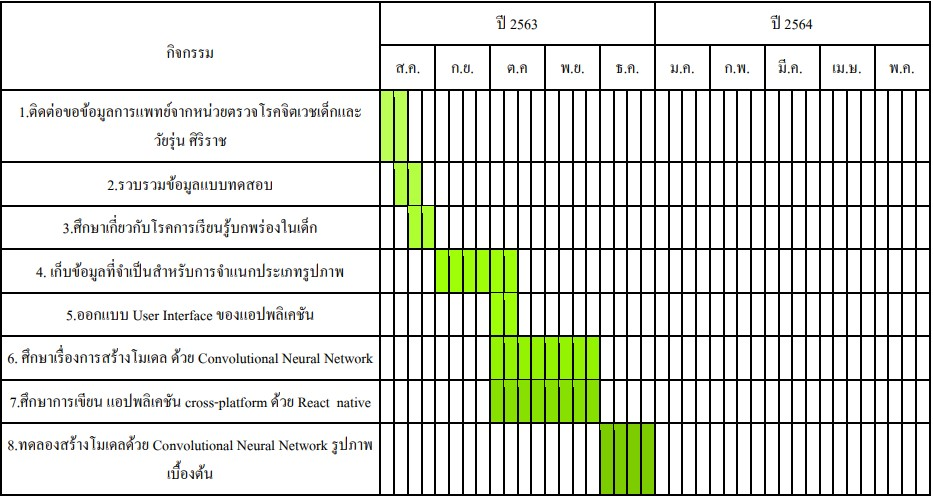
\includegraphics[height=10cm]{./gantt1.jpg}}
  \caption{ภาพตารางเวลาการทำงานภาคการศึกษาที่ 1}\label{fig:system}
 \end{figure}
 \begin{figure}[ht]\centering
  \setlength{\fboxrule}{0.2mm} % can define this in the preamble
  \setlength{\fboxsep}{1cm}
  \fbox{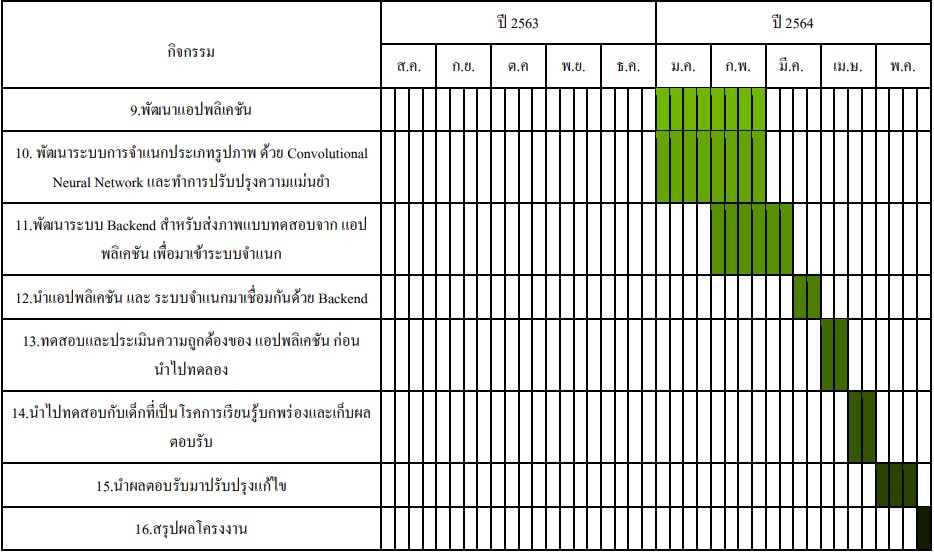
\includegraphics[height=10cm]{./gantt2.jpg}}
  \caption{ภาพตารางเวลาการทำงานภาคการศึกษาที่ 2}\label{fig:system}
 \end{figure}
\end{landscape}
\section{ผลการดำเนินงาน}
\noindent ภาคการศึกษาที่ 1 
\begin{itemize}
  \item ระบบเก็บรวบรวมข้อมูลทดสอบการเขียนของเด็กที่ได้รับบการทดสอบ
  \item ข้อมูลที่ผ่านการประมวลผลที่เตรียมพร้อมสำหรับนำไปสร้างโมเดลในการวิเคราะห์โรคบกพร่องทางการเรียนรู้
  \item โมเดลจำแนกประเภทรูปภาพแบบเบื้องต้นด้วย Convolutional Neural Network
  \item แบบจำลอง User interface ของแอปพลิเคชัน
\end{itemize}
ภาคการศึกษาที่ 2 
\begin{itemize}
  \item ระบบวิเคราะห์รูปภาพลายมือเขียนแบบทดสอบของเด็กเพื่อวินิจฉัยโอกาสเป็นโรคการเรียนรู้บกพร่องเบื้องต้นในเด็กได้อย่างแม่นยำ
  \item แอปพลิเคชัน ที่อยู่ในรูปแบบเกมส์เพื่อให้เด็กเล่น และสามารถทำแบบทดสอบไปพร้อมกันโดยจากนั้นนำภาพไปใช้ในการวินิจฉัยความเป็นไปได้ของโรคการเรียนรู้บกพร่องเบื้องต้น
  \item ผลลัพธ์ที่แม่นยำ และสามารถแสดงถึงจำนวนความผิดพลาดที่เขียนผิด และความน่าจะเป็นได้
  \item ผลประเมินการใช้งานจากผู้ใช้งาน
\end{itemize}
%%%%%%%%%%%%%%%%%%%%%%%%%%%%%%%%%%%%%%%%%%%%%%%%%%%%%%%%%%%%
%%%%%%%%%%%%%%  Literature Review %%%%%%%%%%%%%%%%%%%%%%%%%%
%%%%%%%%%%%%%%%%%%%%%%%%%%%%%%%%%%%%%%%%%%%%%%%%%%%%%%%%%%%%
\chapter{ทฤษฎีความรู้ และงานที่เกี่ยวข้อง}
\section{Core concept แนวคิดหลัก}
เนื่องจากตัวระบบที่ทางคณะผู้จัดทำสร้างขึ้นมาเพื่อวินิจฉัยโรคการเรียนรู้บกพร่องในเด็กนั้นจะต้องทำการเรียนรู้ข้อมูลลักษณะจุดเด่นต่างๆของภาพผลแบบทดสอบการเรียนรู้บกพร่องในเด็กว่า 
มีลักษณะเด่นใดจึงจำแนกว่าเด็กคนนั้นมีโอกาสเป็นโรคการเรียนรู้บกพร่องในเด็ก 
จากการค้นคว้าหาข้อมูลจึงพบว่าเราจำเป็นที่จะต้องใช้ความรู้ในเรื่องของ Convolutional Neural Network 
ซึ่งเหมาะแก่การทำการจำแนกประเภทของรูปภาพ และเป็นส่วนหนึ่งของเรื่องการเรียนรู้เชิงลึกของคอมพิวเตอร์ (deep learning)

\subsection{การเรียนรู้เชิงลึกของคอมพิวเตอร์ (deep learning)}

\par การเรียนรู้เชิงลึกของคอมพิวเตอร์ (deep learning) เป็นหนึ่งในสาขาย่อยของ machine learning เป็นศาสตร์ที่พูดถึงการจำลองการทำงานของระบบโครงข่ายประสาทมนุษย์ โดย จะมีการแบ่งการทำงานข้างในเป็น layer ต่างๆ โดยเราจะมองเป็นสามส่วนหลักๆได้แก่ 	

\begin{enumerate}
  \item Input Layer มีหน้าที่สำหรับการรับข้อมูลป้อนเข้าโครงข่ายประสาท จากผู้ใช้ เช่น รูปภาพ
  \item Hidden Layer มีหน้าที่สำหรับการประเมินข้อมูลที่ป้อนเข้ามา เพื่อหาข้อมูลต่างๆที่ใช้ในการจำแนกประเภทโดยตัว Hidden Layer นั้นสามารถมีได้มากกว่า 1 ชั้น
  \item Output layer เป็นชั้นสุดท้ายมีหน้าที่สำหรับรับข้อมูลจาก Hidden Layer เพื่อใช้ในการบอกว่าท้ายที่สุดแล้วตัวข้อมูลที่รับเข้ามานั้นถูกจำแนกอยู่ในประเภทใด
\end{enumerate}

\begin{figure}[!ht]\centering
  \setlength{\fboxrule}{0.2mm} % can define this in the preamble
  \setlength{\fboxsep}{1cm}
  \fbox{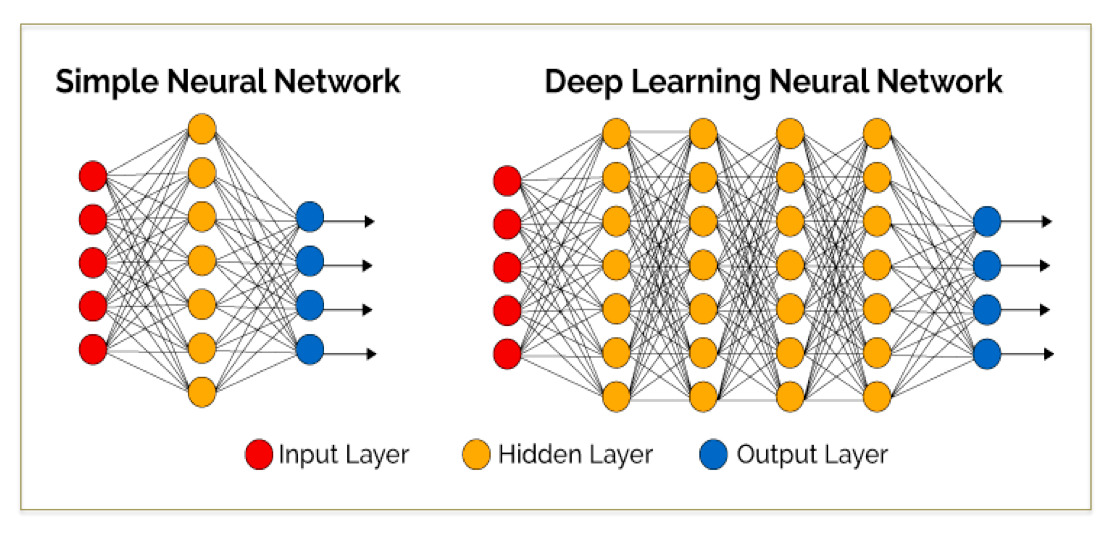
\includegraphics[width=10cm]{./DeepLearning.jpg}}
  \caption{ตัวอย่าง layer ของ การเรียนรู้เชิงลึกของคอมพิวเตอร์}\label{fig:deep}
  \source{[ที่มา: https://verneglobal.com/news/blog/deep-learning-at-scale]}
\end{figure}
\newpage
\subsection{โครงข่ายประสาทเทียมแบบสังวัตนาการ (Convolutional Neural Network)\cite{CS231}} 
\FloatBarrierในปัจจุบันการทำ การจำแนกประเภทรูปภาพ สำหรับทางด้านการแพทย์กำลังเป็นที่สนใจ โครงข่ายประสาทเทียมแบบสังวัตนาการ 
หรือ CNN เลยได้รับความนิยมมากขึ้นโดย CNN เป็นรูปแบบหนึ่งของ การเรียนรู้เชิงลึกของคอมพิวเตอร์ ที่เกิดจากการนำแนวคิดของ  
Neural Network มาเพิ่มในส่วนของ Convolutional layer ซึ่งเหมาะแก่การหาลักษณะต่างๆของข้อมูลต่างๆ เช่น รูปภาพ 
โดยตัวของ CNN นั้นจะประกอบด้วยหลายๆ layer ด้วยกัน

\begin{figure}[!ht]\centering
  \setlength{\fboxrule}{0.2mm} % can define this in the preamble
  \setlength{\fboxsep}{1cm}
  \fbox{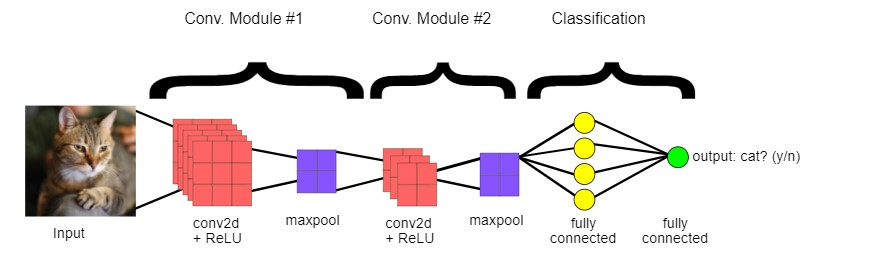
\includegraphics[width=10cm]{./cnn.jpg}}
  \caption{แสดงตัวอย่างโครงข่าย CNN ที่ประกอบด้วย 1. convolutional layer 2. pooling layer 3. fully connected layer
  }\label{fig:cnn}
  \source{[ที่มา: https://developers.google.com/machine-learning/practica/image-classification/convolutional-neural-networks]}
\end{figure}

โดย CNN จะมี layer หลักๆได้แก่ 	
\begin{enumerate}
  \item Convolutional layer ซึ่งมีหน้าที่ในการประมวลผลภาพเพื่อหาคุณลักษณะต่างๆ เช่น สี ขอบ ด้วย filters และนำไปเข้า activate function เพื่อแปลงผลลัพธ์ให้กลายเป็นข้อมูลนำเข้าสำหรับ layer ถัดไป 
  โดยมี activate function ที่ได้รับความนิยมในการทำ การจำแนกประเภทรูปภาพ คือ Rectified Linear Unit (ReLU)
  \item Pooling layer มีหน้าที่ในการลดมิติของข้อมูลที่เราได้จาก Convolutional layer ให้เล็กลง และคงไว้ซึ่งข้อมูลที่จำเป็นเพื่อที่จะทำให้การประมวลผลเร็วขึ้น โดยจะมีสองวิธีหลักๆได้แก่ 
  Max pooling และ Mean pooling โดย Max pooling จะทำการเลือกค่าที่มากที่สุดในขอบเขตที่สนใจ และ Mean Pooling จะทำการหาค่าเฉลี่ยของขอบเขตที่สนใจแล้วนำไปใช้ต่อ ดังรูป \ref{fig:pooling} 
  \begin{figure}[H]\centering
    \setlength{\fboxrule}{0.2mm} % can define this in the preamble
    \setlength{\fboxsep}{1cm}
    \fbox{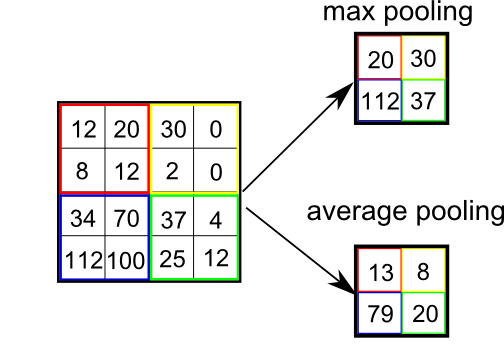
\includegraphics[width=10cm]{./pooling.png}}
    \caption{ตัวอย่างการทำ Max pooling และ mean pooling}\label{fig:pooling}
    \source{[ที่มา: https://stackoverflow.com/questions/44287965]}
  \end{figure}
  \item fully connected layer มีหน้าที่ในการรวบรวม output จาก layer ก่อนหน้า ที่ได้ทำการหา คุณลักษณะต่างๆมารวม และกำหนดให้ผลลัพธ์ของ layer นี้มีจำนวนเท่ากับ จำนวนประเภทที่เราต้องการจำแนกรูปภาพ 
  เพื่อดูว่าผลลัพธ์ท้ายสุดเราจำแนกรูปภาพนั้นได้อยู่ในประเภทไหนซึ่ง CNN จะประกอบด้วยหลายๆ layer นี้เรียงกันไปมาจนถึง output ตามความเหมาะสมของ โมเดลนั้นๆ และสามารถปรับ parameter ของแต่ละ layer ได้เพื่อทำให้การจำแนกประเภทนั้นออกมาแม่นยำที่สุด 
  โดยในโครงการนี้ คณะผู้จัดทำจะเลือกใช้ Convolutional neural network ในการสร้าง โมเดลเพื่อจำแนกข้อมูลภาพถ่าย
\end{enumerate}

\subsection{Transfer Learning\cite{Transfer}}
ในการทำ Convolutional neural networkนั้น เราจำเป็นจะต้องออกแบบตัว layer และ parameter ต่างๆให้เหมาะสมเพื่อให้ได้ความแม่นยำในการจำแนกที่สูง
ซึ่งเราจำเป็นต้องใช้ข้อมูลจำนวนมากในการ train ให้โมเดล CNN ของเรานั้นมีความแม่นยำ แต่ว่า Transfer Learning คือการที่เรานำ โมเดล CNN ที่มีการสร้างขึ้นมาไว้แล้วจากข้อมูลอื่น มาปรับแต่งในส่วนของ
fully connected layer เองใหม่ให้เหมาะสมกับข้อมูลที่เราจะทำการจำแนก ซึ่งจะทำให้ประหยัดเวลาในการสร้างโมเดล และลดจำนวนข้อมูลที่ใช้ในการสร้างโมเดลเพื่อที่จะทำให้โมเดลนั้นมีความแม่นยำ
\begin{figure}[!ht]\centering
  \setlength{\fboxrule}{0.2mm} % can define this in the preamble
  \setlength{\fboxsep}{1cm}
  \fbox{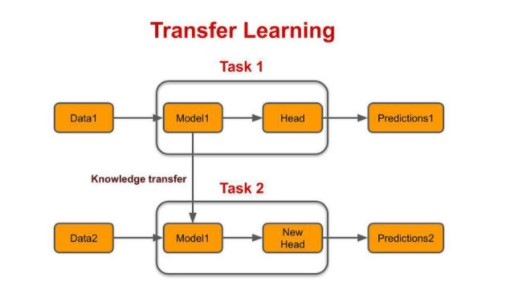
\includegraphics[width=10cm]{./transfer.jpg}}
  \caption{ภาพอธิบายตัวอย่างของ Transfer Learning}\label{fig:transfer}
  \source{[ที่มา: https://www.topbots.com/transfer-learning-in-nlp/]}
\end{figure}

\newpage 
\subsection{Activate Function\cite{Activate}}
Activate function มีหน้าที่ในการปรับผลลัพธ์ ของ neuron ในแต่ละ layer ก่อนจะส่งต่อไปเป็นข้อมูลนำเข้าสำหรับ layer ถัดไป โดย Activate function ที่เป็นที่นิยมคือ sigmoid function เนื่องจากตัว sigmoid function 
น้ันจะมีผลลัพธ์ออกมาอยู่ในช่วงของ 0 จนถึง 1 ทำให้เหมาะแก่การใช้ทำเรื่องความน่าจะเป็น แต่เนื่องจากกราฟของ sigmoid function เป็นดังรูป \ref{fig:sigmoid}  จะเห็นว่าหากค่า |x| มีค่าสูงมากขึ้นค่าของ sigmoid tfunction จะมีการเปลี่ยนแปลงที่น้อยลง 
หรือมีค่าอนุพันธ์ที่น้อยลงทำให้การอัพเดทน้ำหนักของตัว Neural network ใน layer แรกๆนั้นมีค่าน้อยจนอาจทำให้การเรียนรู้หยุด  
ปัญหานี้มีชื่อเรียกว่า Vanishing gradient problem โดยสามารถแก้ไขด้วยการเปลี่ยน activate function ได้ยกตัวอย่างเช่น Rectified Linear Unit หรือ ReLU

\begin{figure}[!ht]\centering
  \setlength{\fboxrule}{0.2mm} % can define this in the preamble
  \setlength{\fboxsep}{1cm}
  \fbox{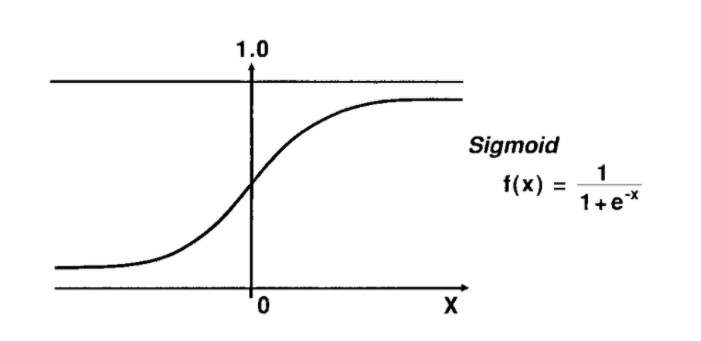
\includegraphics[width=10cm]{./sigmoid.jpg}}
  \caption{ภาพตัวอย่างกราฟของ sigmoid function}\label{fig:sigmoid}
  \source{[ที่มา: https://www.researchgate.net/figure/An-illustration-of-the-signal-processing-in-a-sigmoid-function_fig2_239269767]}
\end{figure}

\subsection{Rectified Linear Unit (ReLU)\cite{ReLuFunc}}
Rectified Linear Unit หรือ ReLU เป็น activate function ที่กำลังได้รับความนิยมเนื่องจากสามารถแก้ไขปัญหาในเรื่องของ 
anishing gradient problem ได้ เพราะกราฟของ ReLU นั้นถ้าค่า x เป็นบวกจะได้ค่าของอนุพันธ์เท่ากับ 1 เสมอทำให้ความชันไม่หาย 
ซึ่งทำให้ตัวโมเดลของนั้นปรับค่าน้ำหนักได้ไวยิ่งขึ้น แต่ก็มีข้อเสียเช่นกันคือผลลัพธ์จะออกมาอยู่ในช่วงตั้งแต่ 0 ถึง อินฟินิตี้ทำให้ไม่สามารถกำหนดขอบเขตได้ หรือผลลัพธ์สำหรับการที่ข้อมูลขาเข้าเป็นเลขติดลบจะเท่ากับ 
0 เสมอทำให้ไม่สามารถแปลงค่าผลลัพธ์ที่เท่ากับ 0 กลับมาเป็นข้อมูลขาเข้าได้ เป็นต้น 


\begin{figure}[!ht]\centering
  \setlength{\fboxrule}{0.2mm} % can define this in the preamble
  \setlength{\fboxsep}{1cm}
  \fbox{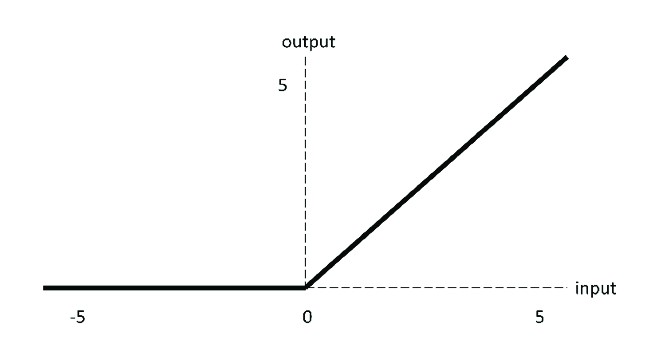
\includegraphics[width=5cm,height=3cm]{./relu.jpg}}
  \caption{ภาพตัวอย่างกราฟของ ReLU function}\label{fig:relu}
  \source{[ที่มา: https://www.researchgate.net/figure/ReLU-activation-function_fig7_333411007]}
\end{figure}



\subsection{การปรับขนาดรูปภาพ (Image rescale)\cite{Imagepre}}
การปรับขนาดรูปภาพ (Image rescale) นั้นเป็นส่วนหนึ่งของกระบวนการเตรียมข้อมูลเบื้องต้นสำหรับการทำโมเดล CNN 
เนื่องมาจากข้อมูลที่ได้มาสำหรับการทำโมเดลนั้น อาจจะมีขนาดที่แตกต่างกันรวมถึงมีขนาดที่ใหญ่เกินไป ด้วยเหตุนั้นจะทำให้โมเดลใช้ระยะเวลาในการเรียนรู้นาน 
คณะผู้จัดทำจึงกำหนดขนาดมาตรฐาน และทำการปรับขนาดข้อมูลรูปภาพสำหรับการสร้างโมเดลก่อนที่จะนำไปใช้

\subsection{การแยกบริเวณรูปภาพ (Image segmentation)\cite{Imagesegment}}
การแยกบริเวณรูปภาพ (Image segmentation) คือการแยกสิ่งที่สนใจออกมาจากพื้นหลังของรูปภาพเพื่อใช้ในการทำโมเดลต่อไป ซึ่งถูกนำไปใช้ประโยชน์ในหลายๆด้านด้วยกันได้แก่ 
การจับตัวหนังสือในภาพ การจับวัตถุแปลกปลอมในรูปภาพเป็นต้น โดยมีหลายรูปแบบด้วยกันยกตัวอย่างเช่น Region-Based Segmetation, Edge Detection Segmentation เป็นต้น
\begin{itemize}
  \item Region-Based Segmentation เป็นการแยกวัตถุออกจากภาพด้วยวิธีการใช้ค่า threshold เพื่อปรับภาพที่อยู่ในรูปแบบของ grayscale ให้กลายเป็น binary image โดยให้วัตถุเป็นหนึ่งสี และ พื้นหลังเป็นอีกสีหนึ่ง เพื่อที่เราจะได้รูปร่างของวัตถุขึ้นมา ซึ่งวิธีการเลือกค่า threshold ที่เหมาะสมมีมากมาย ยกตัยวอย่างเช่น Otsu’s thresholdig method

  \item Edge Detection Segmentation ที่ใช้ในการหาขอบของวัตถุซึ่งใช้หลักการความไม่ต่อเนื่องภายใน pixel ของรูปภาพ โดยจุดที่เกิดการเปลี่ยนแปลงนั้นจะถูกระบุเป็นจุดขอบ 
  \item Output layer เป็นชั้นสุดท้ายมีหน้าที่สำหรับรับข้อมูลจาก Hidden Layer เพื่อใช้ในการบอกว่าท้ายที่สุดแล้วตัวข้อมูลที่รับเข้ามานั้นถูกจำแนกอยู่ในประเภทใด
\end{itemize}
\begin{figure}[!ht]\centering
  \setlength{\fboxrule}{0.2mm} % can define this in the preamble
  \setlength{\fboxsep}{1cm}
  \fbox{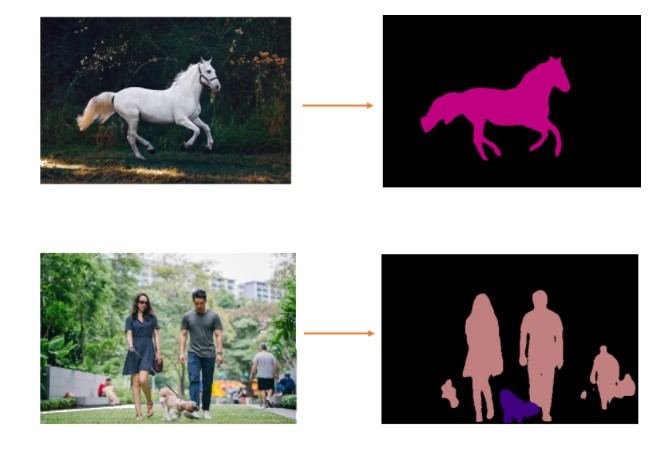
\includegraphics[width=10cm]{./imagesegment.jpg}}
  \caption{ภาพตัวอย่างการทำ image segmentation บนภาพ}\label{fig:imagesegment}
  \source{[ที่มา: https://www.learnopencv.com/applications-of-foreground-background-separation-with-semantic-segmentation/]}
\end{figure}


\newpage
\subsection{การแปลงรูปภาพเป็นข้อความ (Optical character recognition)}
Optical character recognition หรือ OCR คือเทคโนโลยีที่ทำให้สามารถจับตัวอักษรที่อยู่ในภาพถ่ายยกตัวอย่างเช่น ภาพสแกนของเอกสาร หรือ สื่อสิ่งพิมพ์ต่างๆเป็นต้น มาแปลงให้อยู่ในรูปแบบของตัวอักษรดิจิตอล
 ที่สามารถแก้ไขได้ และง่ายต่อการจัดเก็บนำไปใช้ต่อ ซึ่งเราสามารถนำเทคโนโลยีไปประยุกต์ใช้ได้ในหลากหลายด้าน เช่น วิเคราะห์ทะเบียนรถยนต์ ด้านการทำระบบค้นหาข้อมูล หรือระบบจัดเก็บรายละเอียดสินค้า

\begin{figure}[!ht]\centering
  \setlength{\fboxrule}{0.2mm} % can define this in the preamble
  \setlength{\fboxsep}{1cm}
  \fbox{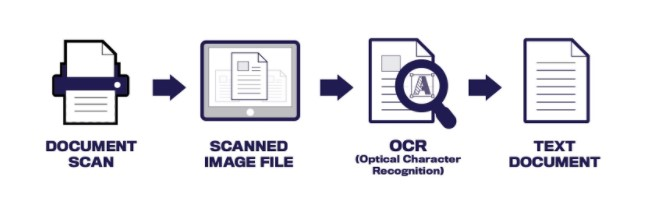
\includegraphics[width=10cm]{./ocr.jpg}}
  \caption{ภาพตัวอย่างขั้นตอนการแปลงเอกสารมาอยู่ในรูปแบบข้อมูลด้วยกระบวนการ OCR}\label{fig:ocr}
  \source{[ที่มา: https://medium.com/states-title/using-nlp-bert-to-improve-ocr-accuracy-385c98ae174c]}
\end{figure}

\subsection{Blob coloring}
ใช้ในการทำ OCR เป็นอัลกอริทึมที่ใช้ในการแบ่งขอบเขตของวัตถุ โดยจะทำการไล่ตั้งแต่ pixel บนสุดของภาพลงมาล่างสุดซึ่งแต่ละ
 pixel จะทำการจับว่า pixel รอบๆตัวนั้นเป็นสีดำหรือไม่ หากเป็นสีดำก็จะจับให้ pixel เหล่านั้นอยู่ใน label เดียวกัน ซึ่งวิธีการนี้จะทำให้สามารถแยกตัวอักษรแต่ละตัวออกจากกันได้ โดยแต่ละตัวก็จะมี label ของตัวมันเอง

\begin{figure}[!ht]\centering
  \setlength{\fboxrule}{0.2mm} % can define this in the preamble
  \setlength{\fboxsep}{1cm}
  \fbox{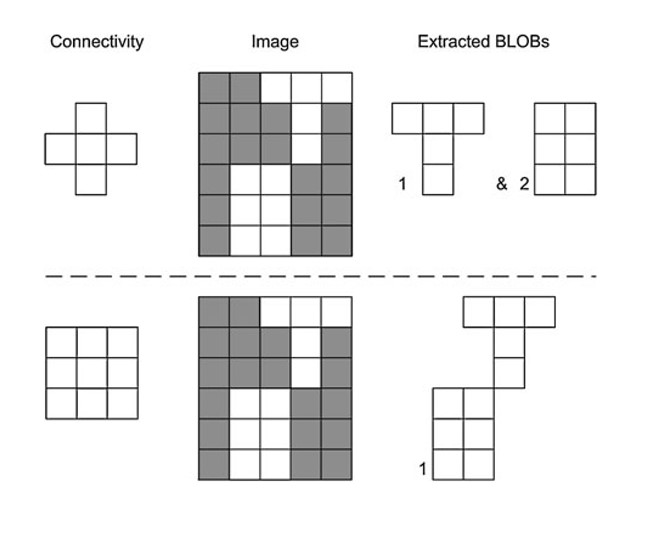
\includegraphics[width=8cm,height=5cm]{./blob.jpg}}
  \caption{ภาพตัวอย่างการทำงานของ Blob coloring}\label{fig:blob}
  \source{[ที่มา: http://what-when-how.com/introduction-to-video-and-image-processing/blob-analysis-introduction-to-video-and-image-processing-part-1/]}
\end{figure}



\section{Languages and technologies ภาษาโปรแกรม และเทคโนโลยี}
เนื่องด้วยด้วยเป้าหมายของโครงการที่่ต้องการพัฒนาแอปพลิเคชันให้สามารถใช้งานได้ในหลายแพลตฟอร์ม 
โดยปัจจุบันระบบปฎิบัติการแอนดรอยด์ และระบบปฎิบัติการไอโอเอสเป็นระบบปฎิบัติการที่ผู้คนใช้งานมากที่สุด 
โดยทั้งสองระบบปฎิบัติการครอบครองส่วนแบ่งทางตลาดมากกว่า 98\%  สำหรับโทรศัพท์มือถือ และแท็ปเล็ต
\begin{figure}[H]\centering
  \setlength{\fboxrule}{0.2mm} % can define this in the preamble
  \setlength{\fboxsep}{1cm}
  \fbox{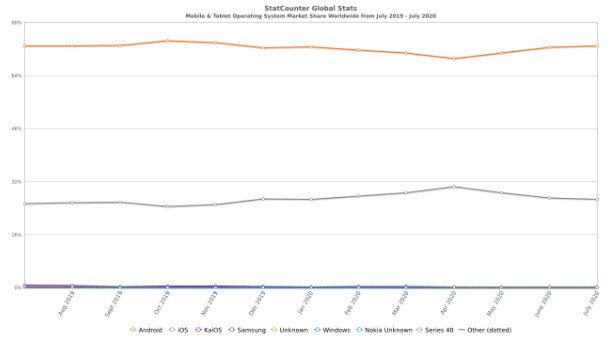
\includegraphics[width=10cm]{./market.jpg}}
  \caption{ส่วนแบ่งการตลาดระบบปฏิบัติการมือถือ และแท็บเล็ตทั่วโลก}\label{fig:market}
  \source{[ที่มา: https://gs.statcounter.com/os-market-share/mobile-tablet/worldwide/#monthly-201907-202007]}
\end{figure}
จากสถิติระบบปฎิบัติการไอโอเอส และระบบปฎิบัติการแอนดรอยด์มีจำนวนผู้ใช้ปริมาณมาก ดังนั้นโครงการจึงพัฒนาแอปพลิเคชันให้สามารถใช้งานได้ทั้งสองระบบปฎิบัติการ 
ซึ่งรูปแบบในการพัฒนาแอปพลิเคชันให้สามารถใช้งานในหลายแพลตฟอร์มได้มีด้วยกันอยู่สองรูปแบบคือ Hybrid Application และ Web Application อย่างไรก็ตาม Hybrid Application 
สามารถทำงานได้ตามเป้าหมายของโครงการมากกว่าเพราะการเป็นรูปแบบแอปพลิเคชันทำให้สามารถใช้หน้าจอสัมผัสผ่านโทรศัพท์มือถือหรือแท็บเล็ตในการเขียนตัวอักษรได้ โดยมีเฟรมเวิร์คให้พัฒนามากมายเช่น React Native ,Ionic และ Flutter เป็นต้น


\subsection{React Native}
React Native คือ เฟรมเวิร์คที่พัฒนาด้วยภาษา JavaScript สำหรับการพัฒนาแอปพลิเคชันสำหรับระบบปฎิบัติการไอโอเอส และระบบปฎิบัติการแอนดรอยด์โดยใช้เทคโนโลยี 
Cross platform ซึ่งในการพัฒนาด้วย React Native มีข้อดีคือในการพัฒนาสามารถพัฒนาแค่ครั้งเดียวแต่สามารถใช้งานได้ทั้งระบบปฎิบัติการไอโอเอส และระบบปฎิบัติการแอนดรอยด์ 
ด้วยการจัดการของ JavaScript ให้สามารถสื่อสารกับฝั่ง Native ของระบบปฎิบัติการทั้งสอง จึงได้ผลลัพธ์ออกมาเป็น Native Application ทั้งระบบปฎิบัติการไอโอเอส และระบบปฎิบัติการแอนดรอยด์ 

\subsection{Keras}
Keras คือเฟรมเวิร์คที่พัฒนาด้วยภาษา Python ที่ถูกสร้างขึ้นมาเพื่อให้สามารถจัดการกับการทำ การเรียนรู้เชิงลึกของคอมพิวเตอร์ (deep learning) 
ได้อย่างง่าย ข้อดีของ Keras คือ ใช้งานง่าย และสามารถดัดแปลงตัว layer ของ neural network ได้ง่าย  โดยในโครงการนี้เราสามารถใช้ Keras 
ในการออกแบบตัว Layer ต่างๆ ของโมเดลได้รวมทั้งทำการสร้างโมเดล และทำนายด้วยภาษา Python ได้เลย

\subsection{OpenCV\cite{OpenCV}}
OpenCV เป็น library ที่มีจุดประสงค์เพื่อการแสดงผลด้วยคอมพิวเตอร์แบบเรียลไทม์  (Real - Time) รวมทั้งในส่วนของการทำ Image processing ที่รองรับการใช้งานบนหลายภาษาด้วยกัน
 โดยหนึ่งในนั้นคือ Python อีกทั้งยังสามารถใช้งานร่วมกับเฟรมเวิร์กการเรียนรู้เชิงลึกต่างๆ อาทิเช่น TensorFlow และ PyTorch  เป็นต้น 

\subsection{Django Rest Framework}
Django Rest Framework เป็น framework ที่พัฒนาขึ้นมาด้วยภาษา python ไว้ใช้สำหรับการสร้าง api ไว้คุยกับฐานข้อมูล  
เพื่อให้ website หรือ application สามารถเรียกใช้ตัว api เพื่อขอข้อมูล  ซึ่งสามารถพัฒนาได้ง่ายด้วยภาษา python
 และที่คณะผู้จัดทำเลือกเนื่องจากตัวโมเดลวินิจฉัยโรคของก็พัฒนาขึ้นจากภาษา python เช่นเดียวกันทำให้สามารถเรียกใช้งานได้ง่าย

\section{Related research/ Competing solutions บทความที่เกี่ยวข้อง}

\subsection{Detecting Dyslexia Using Neural Networks\cite{Dyslexia}}
\begin{figure}[!ht]\centering
  \setlength{\fboxrule}{0.2mm} % can define this in the preamble
  \setlength{\fboxsep}{1cm}
  \fbox{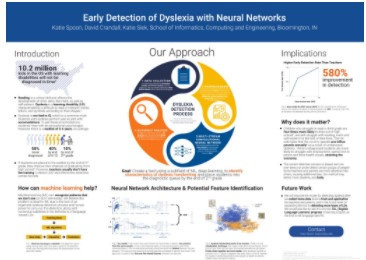
\includegraphics[width=6cm,height=5cm]{./dyslexia.jpg}}
\end{figure}

\subsubsection{การใช้ภาพลายมือในการวินิจฉัยโรค Dyslexia}
มีงานจำนวนมากที่วินิจฉัยโรค Dyslexia โดยการใช้ข้อมูลคะแนนการสอบ ประวัติของผู้ทดสอบ หรือ แบบสอบถาม และมีอีกจำนวนหนึ่งที่ใช้ข้อมูลเช่นภาพการทำงานของสมอง หรือ การสื่อสารผ่านทางดวงตาเป็นต้น 
แต่วรรณกรรมนี้ได้เลือกที่จะใช้ข้อมูลลายมือเนื่องจาก เป็นข้อมูลที่ง่ายต่อการเก็บรวบรวม


\subsubsection{การประมวลผลภาพ}
ในส่วนของการประมวลผลภาพนั้น วรรณกรรมนี้ได้ทำการนำภาพลายมือมาแบ่งเป็นบรรทัด 
หลังจากนั้นจึงได้นำแต่ละบรรทัดมาแบ่งเป็นอีก 50 ส่วน โดยวิธีการที่ใช้ในการแบ่งบรรทัด คือ 
 Arvanitopoulos & Susstrunk’s seam carving แล้วจึงนำภาพแต่ละบรรทัดไปแบ่งเป็น 50 
 ส่วนโดยใช้ขนาด 113*113 ซึ่งยังมีบางภาพที่ยากต่อการทำ แล้วจำเป็นต้องใช้การแก้ไขโดยผู้จัดทำก่อน แต่ไม่ได้มีความยากในการแก้ไขสูง

 \subsubsection{Optical character recognition}
 Optical character recognition หรือ OCR นั้นเป็นการจับตัวอักษรภายในภาพแล้วจึงนำมาแปลงเป็นค่า
  วิธีนี้สามารถอ่านได้ว่าในภาพนั้นมีตัวอักษรตัวใดอยู่บ้าง แต่จากการทดลองของวรรณกรรมนี้พบว่า 
  วิธีนี้ไม่เหมาะสมกับการนำมาอ่านภาพลายมือของเด็กที่เป็นโรค 
  เนื่องจากลายมือของเด็กนั้นมีความหลากหลายมาก ทำให้วิธีการตรวจจับด้วยระบบ OCR ไม่สามารถตรวจจับได้อย่างแม่นยำ
\subsubsection{การทำโมเดลวินิจฉัย}
เป็นส่วนที่ให้โมเดลนั้นได้ทำการระบุว่าข้อมูลที่ป้อนเข้ามาเป็นโรค dyslexia หรือไม่ 
โดยตัวโมเดลนั้นอยู่ในรูปแบบของ  โครงข่ายประสาทเทียมแบบสังวัตนาการ 
หรือ Convolutional Neural Network โดยประกอบด้วย convolutional layer จำนวน 5 layer 
max-pooling จำนวน 3 layer fully-connected จำนวน 2 layer และ dropout layer จำนวน 1 layer 
หลังจากนั้นจึงได้แบ่งข้อมูลแบบ 3:1:1 โดยเป็นข้อมูลในส่วนของการ train 60% test 20% และvalidation 20% และได้ทดลองทำการเรียนรู้โมเดลด้วย batch size และจำนวนส่วนของแถวที่แบ่ง ด้วยหลายๆค่า โดยได้ค่าที่เหมาะสมคือ batch size = 4 และ แบ่ง 50 ส่วนต่อแถวของคำพูด

วรรณกรรมนี้ เป็นวรรณกรรมที่ดี และมีคล้ายกับว่ามีข้อเสนอแนะว่าไม่ควรใช้อะไรบ้าง 
รวมถึงช่วยเรื่องการคิดระบบการทำงานว่าควรมีขั้นตอนแบบใดจากวิธีแรกถึงวิธีสุดท้าย
 เห็นได้ว่ามีหลายวิธีอยากมากที่วินิจฉัยเรื่องของการเป็น LD แต่ว่าโปรเจ็คของเขาได้เลือกวิธีการวินิจฉัย
 ผ่านลายมือเนื่องจากสามารถเก็บรวบรวมได้ง่าย หลังจากนั้นนำภาพมาแบ่งเป็น 50 ส่วนตามขนาด 113*113 
 แต่ก็พบว่ายังมีบางภาพที่สามารถตัดแบ่งได้ยาก และใช้ OCR ในการระบุด้วย ผลออกมาคือมาความแม่นยำที่น้อย







%%%%%%%%%%%%%%%%%%%%%%%%%%%%%%%%%%%%%%%%%%%%%%%%%%%%%55
%%%%%%%%%%%%%%%%%%%%%%%%%%%%%%%%%%%%%%%%%%%%%%%%%%%%%
%%%%%%%%%%%%%%%%%%%%%%%%%%%%%%%%%%%%%%%%%%%%%%%%%%%%%
\chapter{วิธีการดำเนินงาน}
ในส่วนของวิธีการดำเนินงานจะกล่าวถึงขั้นตอนการวางแผนงาน และระบบงานต่างๆ ของแอปพลิเคชัน แอลดีสปอต โดยจะประกอบด้วยหัวข้อต่างๆ ได้แก่ System Architecture, System Requirement, Process flow, Use cases, โครงสร้างซอฟต์แวร์, Conceptual Design, Database Design, Sequence Diagram Design, User Interface Design และการเก็บภาพลายมือเด็ก
\section{Project Functionality}
\subsection{System Architecture}
\begin{figure}[!ht]\centering
  \setlength{\fboxrule}{0.2mm} % can define this in the preamble
  \setlength{\fboxsep}{1cm}
  \fbox{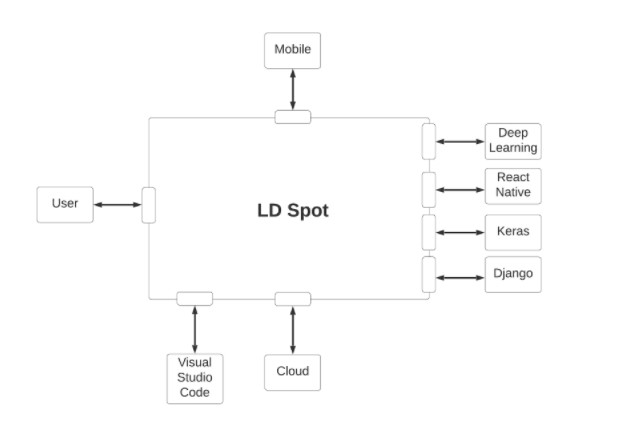
\includegraphics[width=10cm]{./system.jpg}}
  \caption{ภาพ System Architecture ของ แอลดีสปอต}\label{fig:system}
\end{figure}
\subsection{System requirements}
\begin{itemize}
  \item รองรับระบบปฏิบัติการแอนดรอยด์ตั้งแต่ 4.1 ขึ้นไป
  \item รองรับระบบปฏิบัติการไอโอเอสตั้งแต่ 10.0 ขึ้นไป
  \item รองรับระบบสัมผัสหน้าจอ
  \item รองรับเฉพาะระบบภาษาไทย
  \item สามารถดูผลการวินิจฉัยย้อนหลังได้
  \item อนุญาติให้เก็บผลการวินิจฉัยบนระบบได้
  \item ผลลัพธ์อยู่ในรูปของคววามน่าจะเป็น และคะแนนความถูกต้องของการเขียน
  \item ต้องใช้อินเทอร์เน็ตในการทำแบบทดสอบผ่านแอปพลิเคชัน
\end{itemize}
\newpage
\subsection{Process Flow}
\begin{figure}[!ht]\centering
  \setlength{\fboxrule}{0.2mm} % can define this in the preamble
  \setlength{\fboxsep}{1cm}
  \fbox{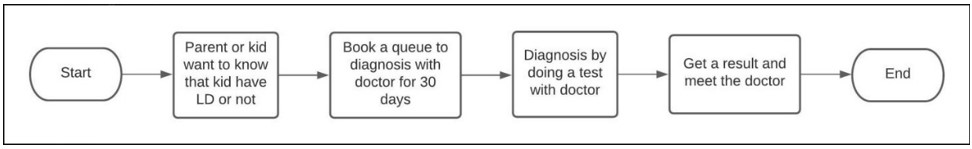
\includegraphics[width=14cm]{./processflowbefore.jpg}}
  \caption{ภาพขั้นการทำงานของบุคลากรทางการแพทย์ก่อนใช้แอปพลิเคชัน แอลดีสปอต}\label{fig:usecase}
\end{figure}
\begin{itemize}
  \item เริ่มด้วยการที่ผู้ปกครองของเด็กหรือตัวเด็กสงสัยว่าเด็กเป็นโรคบกพร่องทางการเรียนรู้หรือไม่ 
  \item ทำการจองคิวสำหรับการวินิจฉัย และรอคิวเป็นระยะเวลา 30 วัน
  \item ทำการทดสอบวินิจฉัยกับบุคลการณ์ทางการแพทย์ 
  \item พบแพทย์ และรับฟังผลลัพธ์
\end{itemize}
\begin{figure}[!ht]\centering
  \setlength{\fboxrule}{0.2mm} % can define this in the preamble
  \setlength{\fboxsep}{1cm}
  \fbox{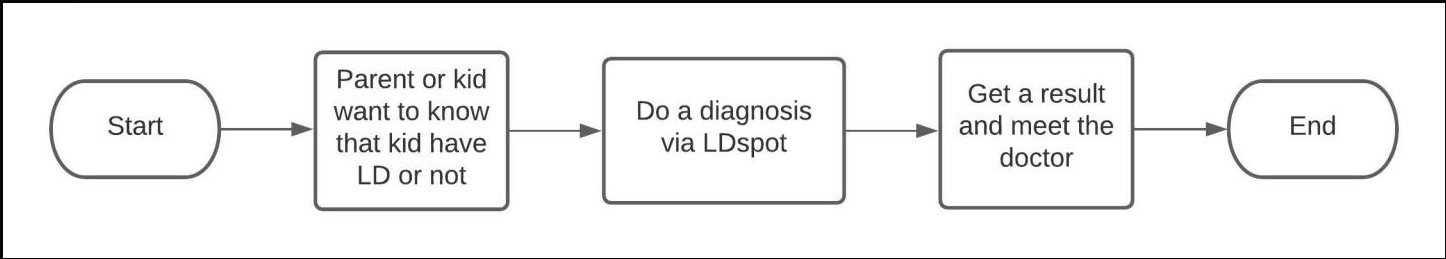
\includegraphics[width=7cm]{./processflowafter.jpg}}
  \caption{ภาพขั้นตอนการทำงานของบุคลากรทางการแพทย์หลังใช้แอปพลิเคชัน แอลดีสปอต}\label{fig:usecase}
\end{figure}
\begin{itemize}
  \item เริ่มด้วยการที่ผู้ปกครองของเด็กหรือตัวเด็กสงสัยว่าเด็กเป็นโรคบกพร่องทางการเรียนรู้หรือไม่ 
  \item ทำการจองคิวสำหรับการวินิจฉัย และรอคิวเป็นระยะเวลา 30 วัน
  \item ทำแบบทดสอบผ่านแอปพลิเคชัน แอลดีสปอต  
  \item พบแพทย์ และรับฟังผลลัพธ์
  \item สามารถติดตามผลลัพธ์ผ่านแอปพลิเคชันได้ รวมถึงสามารถทำแบบทดสอบใหม่ได้เพื่อติดตามพัฒนาการ
\end{itemize}
\newpage
\subsection{Use cases}
\begin{figure}[!ht]\centering
  \setlength{\fboxrule}{0.2mm} % can define this in the preamble
  \setlength{\fboxsep}{1cm}
  \fbox{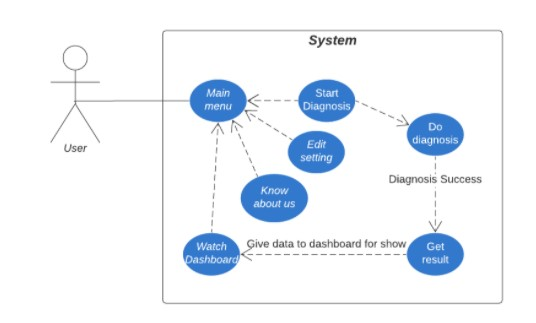
\includegraphics[scale=0.5]{./usecase.jpg}}
  \caption{ภาพ Use Case Diagram}\label{fig:usecase}
\end{figure}
แสดงถึงแผนภาพฟังก์ชั่นการทำงานของระบบโดยมีผู้ใช้งานใน 2 บทบาทหลัก ได้แก่ Personnel คือบุคลากรทางการแพทย์ และ child คือเด็กหรือผู้ทำแบบทดสอบโดยแยกเป็นกรณีดังนี้
\begin{itemize}
  \item ในส่วนของบุคลากรทางการแพทย์ จะสามารถเข้าสู่ระบบโดยจะสามารถกรอกเลขผู้ทำแบบทดสอบเพื่อเริ่มทำแบบทดสอบได้ โดยจะสามารถทำซ้ำได้เรื่อยๆ เมื่อทำเสร็จแล้ว แอปพลิเคชันจะแสดงผลลัพธ์ของแบบทดสอบในหน้าผลลัพธ์โดยบุคลากรทางการแพทย์จะสามารถดูผลลัพธ์ได้เพื่อประกอบการวินิจฉัย และสังเกตพัฒนาการของผู้ทำแบบทดสอบ โดยที่บุคลากรทางการแพทย์สามารถดูได้ว่าตัวอักษร สระ และคำสะกดใดๆที่ผู้ทำแบบทดสอบนั้นได้เขียนถูกจำแนกออกมาเป็น ถูก ผิด กลับด้าน อย่างไร และสามารถแก้ไขการจำแนก 
  ถูก ผิด กลับด้านได้ หากแอปพลิเคชันจำแนกผิดพลาด ในส่วนของบอร์ดสถิติบุคลากรทางการแพทย์สามารถดูสถิติโดยรวมของผู้เข้าทำแบบทดสอบผ่านแอปพลิเคชันได้ เช่น ตัวอักษรที่ผู้ทำแบบทดสอบมักจะเขียนผิดเป็นต้น 
  \item ในส่วนของผู้ทำแบบทดสอบ จะสามารถทำได้เพียงเริ่มทำแบบทดสอบเพียงเท่านั้น 
\end{itemize}

\section{โครงสร้างซอฟต์แวร์}
ในส่วนของการใช้งานระบบ แอลดีสปอต นั้นจะแบ่งเป็นสี่ส่วนหลักๆได้แก่ แอปพลิเคชันทำแบบทดสอบ การประมวลผลภาพ การแยกภาพ การวินิจฉัย โดยมีขั้นตอนของตัวระบบดังนี้
\begin{enumerate}
  \item ผู้ใช้จะต้องทำแบบทดสอบภายในแอปพลิเคชันโดยจะอยู่ในรูปแบบของเกมเขียน พยัญชนะ สระ และ สะกดคำ
  \item หลังจากนั้นภาพแบบทดสอบที่ผู้ใช้ได้ทำจะถูกส่งเข้าไปภายในระบบ LDSpoแอลดีสปอตt เพื่อทำการปรับปรุงคุณภาพของรูปภาพได้แก่การปรับขนาดของภาพให้เหมาะสม การลดสัญญาณรบกวนในภาพ และการปรับสีให้อยู่ในรูปแบบของขาวดำ
  \item เมื่อได้ภาพที่ผ่านการทำการปรับปรุงคุณภาพของภาพแล้ว ภาพที่เป็นตัวอักษร และสระจะถูกนำส่งไปวินิจฉัย เพื่อดูผลลัพธ์ว่าเขียนถูกหรือไม่ ส่วนภาพตัวสะกดจะถูกส่งไปเข้ากระบวนการ OCR เพื่อแยกออกมาเป็นตัวอักษร และสระเดี่ยวๆ จากนั้นจึงนำ ตัวอักษร และสระเดี่ยวๆทั้งหมดจากกระบวนการ OCR ไปวินิจฉัยว่าตรงกับคำสะกดนั้นหรือไม่
  \item นำภาพแต่ละตัวอักษรเข้าไปวินิจฉัย เพื่อนำผลลัพธ์จากโมเดลมาแสดงผลบนแอปพลิเคชัน
\end{enumerate}

\end{itemize}
\newpage
\begin{figure}[!ht]\centering
  \setlength{\fboxrule}{0.2mm} % can define this in the preamble
  \setlength{\fboxsep}{1cm}
  \fbox{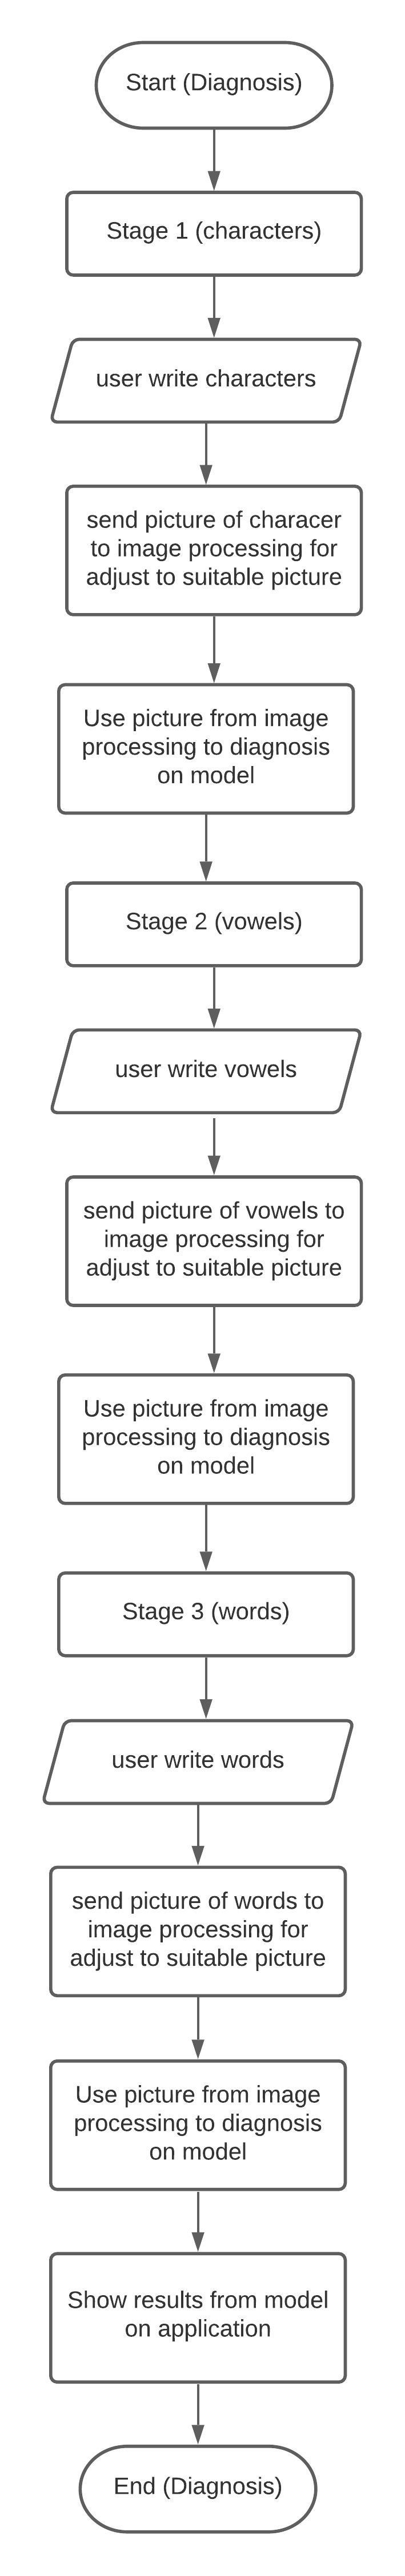
\includegraphics[scale=0.5]{./fcProcessLDsenior.jpeg}}
  \caption{ภาพ Activity diagram การดูข้อมูลสถิติในแอปพลิเคชัน}\label{fig:activity3}
 \end{figure}
 \newpage
\subsection{แอปพลิเคชันทำแบบทดสอบ (Application)}
ในส่วนของแอปพลิเคชันทำแบบทดสอบนั้นเพื่อที่จะได้มาซึ่งภาพแบบทดสอบคณะผู้จัดทำจึงออกแบบแอปพลิเคชันส์ในรูปแบบของเกมให้ผู้ใช้ทำ ซึ่งในส่วนนี้ผู้ใช้จะต้องทำแบบทดสอบการเขียนพยัญชนะ สระ และสะกดคำ โดยจะมีกรอบขึ้นมาให้ผู้ใช้เขียนตามเสียงพูด 
\begin{table}[!h]\centering
  \caption{แสดงข้อมูลขาเข้า และขาออกของ แอปพลิเคชัน}\label{tbl:application1}
  \begin{tabular}{c|c|l|rr} \hline
  Input & ผู้ใช้ทำแบบทดสอบภายในแอปพลิเคชัน \\ \hline
  Output & ภาพแบบทดสอบการเขียนพยัญชนะ สระ และ คำสะกด \\ \hline
  \end{tabular}
  \end{table}

\subsection{การประมวลผลภาพ (Image processing)}
ในส่วนนี้นั้นคณะผู้จัดทำจะนำภาพแบบทดสอบที่ได้จากแอปพลิเคชันมาปรับปรุงคุณภาพของภาพเพื่อให้เหมาะสมแก่การนำไปวินิจฉัย โดยจะมีการปรับขนาดของภาพให้ตรงกับขนาดของภาพที่ระบบ 
แอลดีสปอต นั้นใช้ในการเรียนรู้ หลังจากนั้นจึงนำภาพไปทำการลดสัญญาณรบกวนด้วยวิธีการใช้ Gaussian blur และจึงปรับภาพให้อยู่ในสีขาวดำ เพื่อแยกตัวอักษรออกจากภาพพื้นหลัง
\begin{figure}[!ht]\centering
  \setlength{\fboxrule}{0.2mm} % can define this in the preamble
  \setlength{\fboxsep}{1cm}
  \fbox{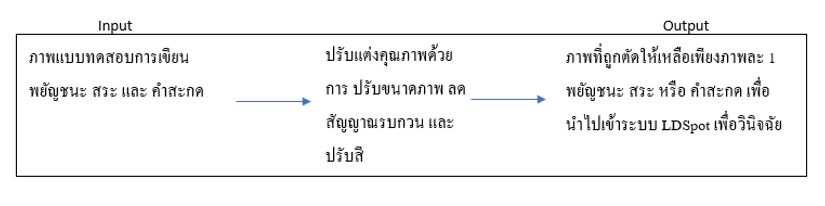
\includegraphics[width=12cm]{./imageprocess.jpg}}
  \caption{แผนภาพแสดงข้อมูลขาเข้า และออกของการประมวลผลภาพ}\label{fig:system}
\end{figure}
\begin{table}[!h]\centering
  \caption{แสดงข้อมูลขาเข้า และขาออกของส่วนการประมวลผลภาพ}\label{tbl:application1}
  \begin{tabular}{c|c|l|rr} \hline
  Input & ภาพแบบทดสอบการเขียนพยัญชนะ สระ และ คำสะกด \\ \hline
  Output & ภาพแบบทดสอบการเขียนพยัญชนะ สระ และ คำสะกดที่ปรับปรุงคุณภาพสำหรับการทำโมเดลแล้ว \\ \hline
  \end{tabular}
  \end{table}
  

  \subsection{การแยกภาพ (Image segmentation)}
  ในส่วนนี้คณะผู้จัดทำจะทำการสร้าง contour ขึ้นมาจากภาพที่ได้ทำการปรับสีขาวดำแล้ว โดยจะนำ contour นั้นไปสร้าง bounding box 
  เพื่อครอบแต่ละตัวอักษรให้แยกออกจากกัน เนื่องจากคณะผู้จัดทำต้องการภาพตัวอักษรที่อยู่เดี่ยวๆ ไปใช้เป็นข้อมูลสำหรับแพทย์ในการวินิจฉัยโรคบกพร่องทางการเรียนรู้ 
  \begin{figure}[!ht]\centering
    \setlength{\fboxrule}{0.2mm} % can define this in the preamble
    \setlength{\fboxsep}{1cm}
    \fbox{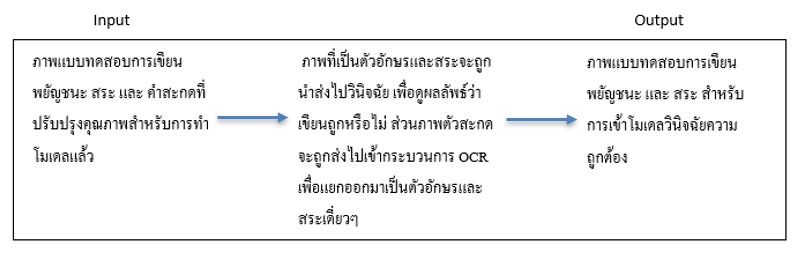
\includegraphics[width=12cm]{./imagesegment3.jpg}}
    \caption{แผนภาพแสดงข้อมูลขาเข้า และออกของการแยกภาพ}\label{fig:system}
   \end{figure}
  \begin{table}[!h]\centering
    \caption{แสดงข้อมูลขาเข้า และขาออกของส่วนการแยกภาพ}\label{tbl:application1}

    \begin{tabular}{c|c|l|rr} \hline
    Input & ภาพแบบทดสอบการเขียนพยัญชนะ สระ และ คำสะกดที่ปรับปรุงคุณภาพสำหรับการทำโมเดลแล้ว  \\ \hline
    Output & ภาพแบบทดสอบการเขียนพยัญชนะ และ สระ สำหรับการเข้าโมเดลวินิจฉัยความถูกต้อง \\ \hline
    \end{tabular}
    \end{table}

  \newpage
  \subsection{การวินิจฉัย (Learning disorder prediction)}
  เมื่อคณะผู้จัดทำได้ภาพตัวอักษรเดี่ยวๆจากส่วนการแยกภาพแล้ว คณะผู้จัดทำจะนำภาพตัวอักษรเดี่ยวๆนั้นไปโยนเข้าโมเดลที่ได้ทำการสร้างไว้ เพื่อให้โมเดลวินิจฉัยว่าภาพตัวอักษร สระ และคำสะกดนั้น ถูกต้องหรือไม่ 
   แล้วนำผลลัพธ์ส่งกลับไปในฐานข้อมูลเพื่อให้แอปพลิเคชันสามารถเรียกข้อมูลไปแสดงได้ต่อไป 
  \begin{figure}[!ht]\centering
    \setlength{\fboxrule}{0.2mm} % can define this in the preamble
    \setlength{\fboxsep}{1cm}
    \fbox{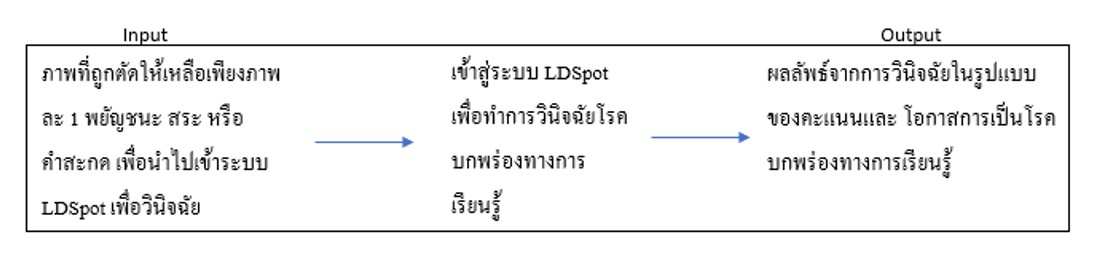
\includegraphics[width=12cm]{./imagepredict3.jpg}}
    \caption{แผนภาพแสดงข้อมูลขาเข้า และออกของการวินิจฉัย}\label{fig:system}
   \end{figure}
  \begin{table}[!h]\centering
    \caption{แสดงข้อมูลขาเข้า และขาออกของส่วนการวินิจฉัย}\label{tbl:application1}
    \begin{tabular}{c|c|l|rr} \hline
    Input & ภาพที่ถูกตัดให้เหลือเพียง ภาพละ 1 พยัญชนะ สระ หรือ คำสะกด เพื่อนำไปเข้าระบบ แอลดีสปอต เพื่อวินิจฉัย  \\ \hline
    Output & ผลลัพธ์จากการวินิจฉัยในรูปแบบของคะแนนเขียนถูก เขียนผิด เขียนกลับด้าน \\ \hline
    \end{tabular}
    \end{table}
\newpage
\section{Conceptual  Design}
\begin{figure}[!ht]\centering
  \setlength{\fboxrule}{0.2mm} % can define this in the preamble
  \setlength{\fboxsep}{1cm}
  \fbox{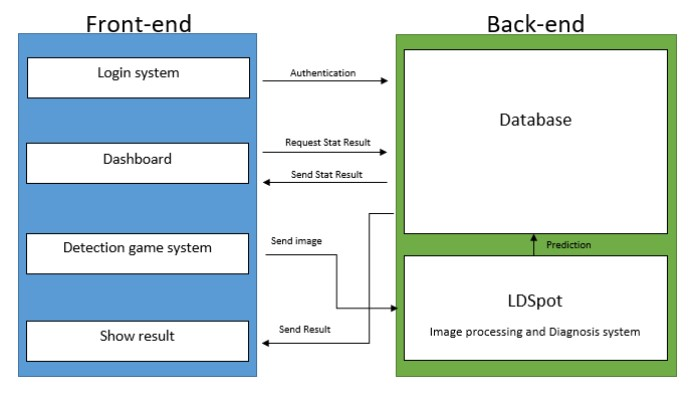
\includegraphics[width=11cm]{./conceptual.jpg}}
  \caption{ภาพการสื่อสารระหว่างทางฝั่ง Frontend และ Backend}\label{fig:conceptual}
 \end{figure}
 อธิบายได้ว่าการทำงานของตัวระบบ แอลดีสปอต นั้นจะมีอยู่สองส่วนด้วยกันได้แก่ front-end ที่ทำหน้าที่เป็นหน้าแอปพลิเคชันไว้สื่อสารกับผู้ใช้งาน
  และส่วนของ back-end ที่รับข้อมูลมาเพื่อประมวลผลแล้วหลังจากนั้นจึงนำข้อมูลไปเก็บใส่ฐานข้อมูลไว้ใช้งานต่อไป 
 \begin{itemize}
   \item ในส่วนของ front-end นั้นจะประกอบไปด้วย แอปพลิเคชันในรูปแบบของเกม โดยที่ผู้ใช้จะสามารถเข้าสู่ระบบผ่านทางรหัสที่ได้ทำการสมัครสมาชิกไว้
    โดยตัวรหัสจะถูกส่งไปเพื่อตรวจสอบความถูกต้องว่ามีรหัสนี้อยู่จริงในระบบหรือไม่กับฐานข้อมูลที่อยู่ภายในส่วนของ back-end หากตรวจสอบแล้วถูกต้องจึงจะสามารถเข้าสู่ระบบได้ 
   \item ผู้ใช้สามารถกดเข้ารับแบบทดสอบได้ โดยเมื่อเข้ารับแล้ว จะต้องทำตามข้ันตอนต่อไป ซึ่งผู้ใช้จะได้เขียนตัวอักษร สระ และคำสะกด ตามเสียงไปเรื่อยๆ เมื่อเสร็จสิ้นแล้วภาพแบบทดสอบจะถูกส่งไปทางฝั่ง back-end 
   ในส่วนของระบบ 
    เพื่อทำการวินิจฉัยหลังจากนั้นผลลัพธ์จะถูกส่งเก็บเข้าไปในฐานข้อมูล เพื่อให้ทางฝั่ง front-end สามารถดึงข้อมูลไปแสดงผลบนแอปพลิเคชันได้
   \item ผู้ใช้สามารถดูผลลัพธ์ย้อนหลังได้โดยกดดูผลลัพธ์ภายในแอปพลิเคชันหลังจากนั้น แอปพลิเคชันจะทำการติดต่อกับฐานข้อมูลเพื่อดึงผลลัพธ์ที่เคยได้มีการวินิจฉัยไว้ของผู้ใช้งานคนนั้นมาแสดงผลว่ามีเขียนพยัญชนะ สระ และคำสะกด ว่า ถูกผิด หรือกลับด้านกี่ตัว
   \item ผู้ใช้สามารถดูบอร์ดสถิติได้ โดยบอร์ดสถิตินั้นจะดึงข้อมูลสรุปจากฐานข้อมูลมาว่า มีผู้ใช้งานแอปพลิเคชันนี้แล้วกี่คน  เพื่อใช้เป็นข้อมูลในเชิงสถิติต่อไป
 \end{itemize}

\begin{landscape}
\section{Database Design}
\begin{figure}[!ht]\centering
    \setlength{\fboxrule}{0.2mm} % can define this in the preamble
    \setlength{\fboxsep}{1cm}
    \fbox{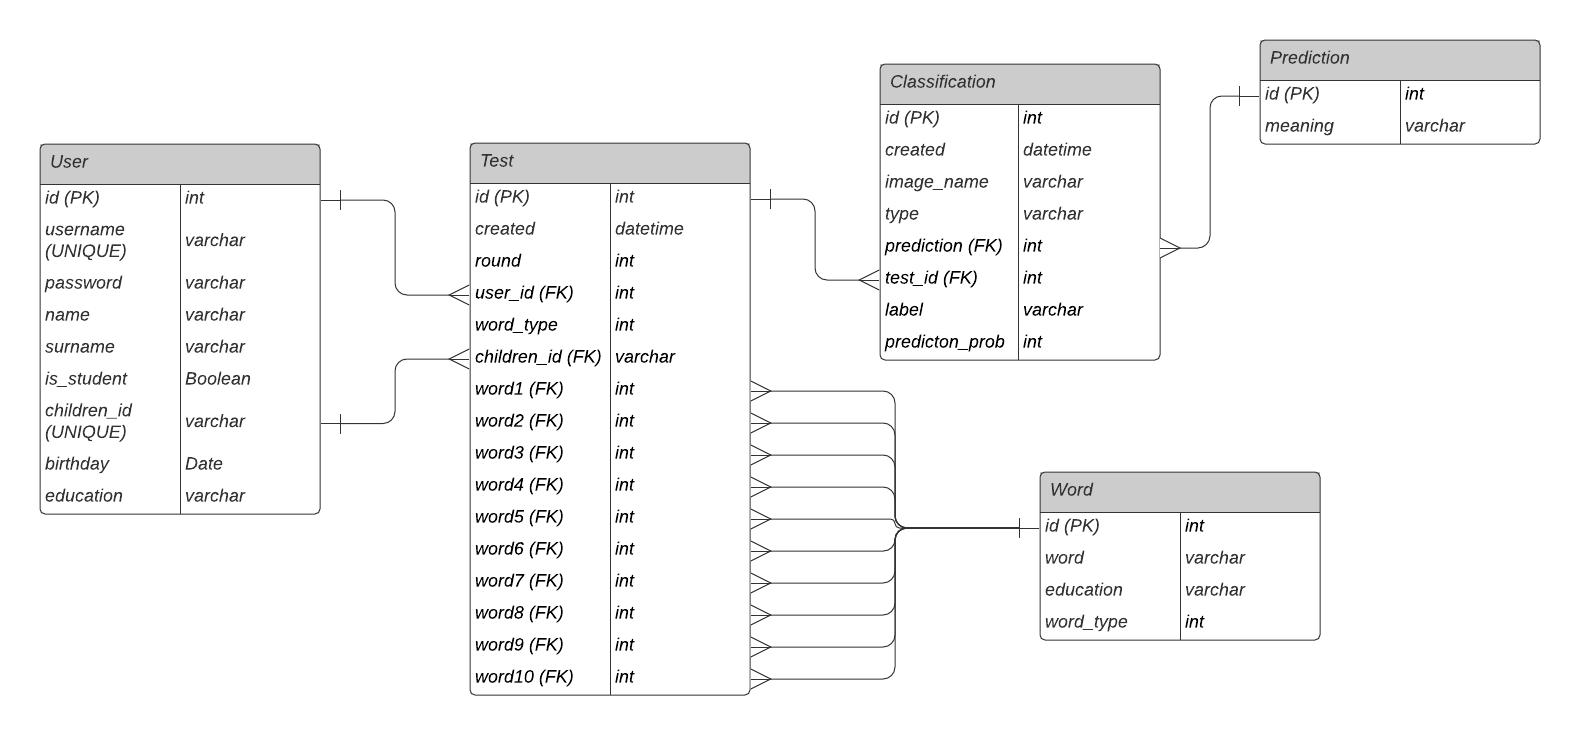
\includegraphics[scale=0.8]{./LDProject - Database Diagram.png}}
    \caption{ภาพ Database ER diagram}\label{fig:database}
   \end{figure}
  \end{landscape}

  Entity User
  \begin{table}[!h]\centering
    \caption{ตารางเก็บข้อมูล User}\label{tbl:application1}
    \begin{tabular}{|p{2cm}|p{2cm}|p{7cm}|p{2cm}|} \hline
      Field & Type & Meaning & Allow Null \\ \hline
      id & int & รหัสผู้ใช้งาน & No \\ \hline
      username & varchar & รหัสสำหรับเข้าสู่ระบบ &No \\ \hline
      password & varchar & รหัสผ่านสำหรับเข้าสู่ระบบ & No \\ \hline
      name & varchar & ชื่อจริง & No \\ \hline
      surname & varchar & นามสกุล & No \\ \hline
      is\_student & Boolean & ระบุสถานะนักเรียน (1,0) & No \\ \hline
      children\_id & varchar & รหัสประจำตัวผู้ทำแบบทดสอบ & No \\ \hline
      birthday & Date & วันเกิด & No \\ \hline
      education & varchar & ระดับการศึกษา (1,2,3,4,5,6) & No \\ \hline
    \end{tabular}
    \end{table}

    Entity Test
    \begin{table}[!h]\centering
      \caption{ตารางเก็บข้อมูล Test}\label{tbl:application1}
      \begin{tabular}{|p{2cm}|p{2cm}|p{7cm}|p{2cm}|} \hline
        Field & Type & Meaning & Allow Null \\ \hline
        id & int & รหัสแบบทดสอบ & No \\ \hline
        created & datetime & เวลาเริ่มทำแบบทดสอบ &No \\ \hline
        round & int & รอบที่ทำแบบทดสอบ & No\\ \hline
        user\_id & int & รหัสผู้เริ่มทำแบบทดสอบ & No \\ \hline
        word\_type & int & ประเภทของคำสะกดในแบบทดสอบ & No \\ \hline
        children\_id & varchar & รหัสประจำตัวผู้ทำแบบทดสอบ (1,0) & No \\ \hline
        word1 & int & รหัสคำสะกด & No \\ \hline
        word2 & int & รหัสคำสะกด & No \\ \hline
        word3 & int & รหัสคำสะกด & No \\ \hline
        word4 & int & รหัสคำสะกด & No \\ \hline
        word5 & int & รหัสคำสะกด & No \\ \hline
        word6 & int & รหัสคำสะกด & No \\ \hline
        word7 & int & รหัสคำสะกด & No \\ \hline
        word8 & int & รหัสคำสะกด & No \\ \hline
        word9 & int & รหัสคำสะกด & No \\ \hline
        word10 & int & รหัสคำสะกด & No \\ \hline
      \end{tabular}
      \end{table}

      Entity Classification
      \begin{table}[!h]\centering
        \caption{ตารางเก็บข้อมูล Classification}\label{tbl:application1}
        \begin{tabular}{|p{2cm}|p{2cm}|p{7cm}|p{2cm}|} \hline
          Field & Type & Meaning & Allow Null \\ \hline
          id & int & รหัสภาพแบบทดสอบ & No \\ \hline
          created & datetime & เวลาเริ่มทำแบบทดสอบ &No \\ \hline
          image\_name & varchar & ที่อยู่ภาพแบบทดสอบ & No \\ \hline
          type & varchar & ชนิดของภาพแบบทดสอบ (alphabet,vowel,vocab) & No \\ \hline
          prediction & int & รหัสคำทำนายภาพแบบทดสอบ (0,1,2,3) & No \\ \hline
          test\_id & int & รหัสแบบทดสอบ & No \\ \hline
          label & varchar & ตัวอักษร สระ หรือคำสะกด ของภาพแบบทดสอบ & No \\ \hline
          prediction\_prob & int & ความน่าจะเป็นของการทำนายภาพแบบทดสอบถูก & No \\ \hline
        \end{tabular}
        \end{table}

        \newpage
        Entity Prediction
        \begin{table}[!h]\centering
          \caption{ตารางเก็บข้อมูล Prediction}\label{tbl:application1}
          \begin{tabular}{|p{2cm}|p{2cm}|p{7cm}|p{2cm}|} \hline
            Field & Type & Meaning & Allow Null \\ \hline
            id & int & รหัสคำทำนายภาพแบบทดสอบ & No \\ \hline
            meaning & varchar & ความหมายของรหัส &No \\ \hline
           
          \end{tabular}
          \end{table}

          
        Entity Word 
        \begin{table}[!h]\centering
          \caption{ตารางเก็บข้อมูล Prediction}\label{tbl:application1}
          \begin{tabular}{|p{2cm}|p{2cm}|p{7cm}|p{2cm}|} \hline
            Field & Type & Meaning & Allow Null \\ \hline
            id & int & รหัสคำสะกด & No \\ \hline
            word & varchar & คำสะกด &No \\ \hline
            education & varchar & ระดับการศึกษา (1,2,3,4,5,6) & No \\ \hline
            word\_type & int & ประเภทของคำสะกด &No \\ \hline
          \end{tabular}
          \end{table}
\newpage
\section{Sequence Diagram Design}
   \begin{itemize}
    \item ทำแบบทดสอบ 
    Sequence diagram นี้อธิบายขั้นตอนการทำแบบทดสอบโดยในขั้นต้นผู้ทดสอบจะต้องเข้าสู่ระบบผ่านทางแอปพลิเคชัน 
    จากนั้นกดเริ่มทำแบบทดสอบทุกครั้งที่มีการเขียนตัวอักษร สระ หรือคำสะกดลงไปแล้วส่งคำตอบ ภาพจะถูกส่งไปที่เซิฟเวอร์ผ่านทาง Django และนำภาพนั้นไปเข้าสู่โมเดลทำนายว่าภาพนั้นเขียนถูกผิด หรือกลับด้านหรือไม่ จากนั้นนำผลลัพธ์ไปเก็บในฐานข้อมูล เพื่อ ที่ท้ายที่สุดหลังจบแบบทดสอบแล้ว 
     จะสามารถนำผลลัพธ์มาสรุปดูได้ว่า มีการเขียนถูกผิดกลับด้านกี่ตัว 
    \begin{figure}[!ht]\centering
      \setlength{\fboxrule}{0.2mm} % can define this in the preamble
      \setlength{\fboxsep}{1cm}
      \fbox{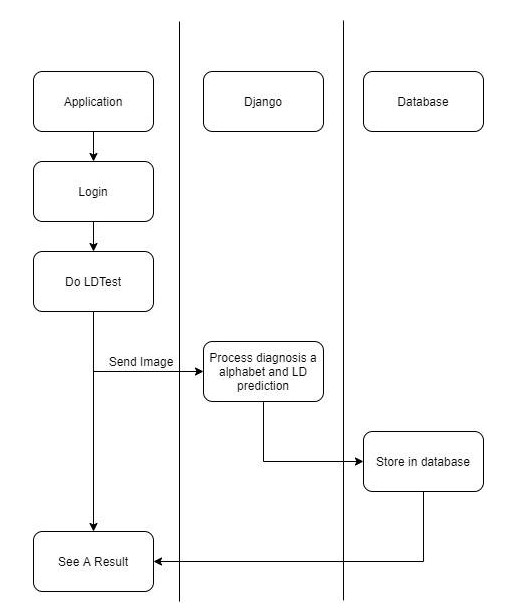
\includegraphics[width=10cm]{./activitytest.jpg}}
      \caption{ภาพ Sequence diagram การทำแบบทดสอบ}\label{fig:activity1}
     \end{figure}
     \newpage
     \begin{table}[!h]\centering
      \caption{Use case narrative ของการทำแบบทดสอบ}\label{tbl:application1}
      \begin{tabular}{|p{4cm}|p{10cm}|} \hline
      Use Case Name & การทำแบบทดสอบ \\ \hline
      Goal in Context & เพื่อให้ได้ภาพตัวอักษร สระ และคำสะกดด้วยลายมือเด็ก \\ \hline
      Primary Actor & ผู้เข้ารับการทำแบบทดสอบ \\ \hline
      Secondary Actor & บุคลากรทางการแพทย์ \\ \hline
      Precondition & ต้องเข้าสู่ระบบก่อน \\ \hline
      Trigger & บุคลากรทางการแพทย์ต้องกรอกชื่อผู้เข้ารับการทดสอบแล้วกดเริ่มการทดสอบ \\ \hline
      Scenario & \begin{enumerate}
        \item บุคลากรทางการแพทย์กดเข้าสู่หน้าเข้ารับการทดสอบ
        \item บุคลากรทางการแพทย์กรอกรหัส ชื่อ นามสกุล ของผู้เข้ารับแบบทดสอบ
        \item ผู้เข้ารับแบบทดสอบเริ่มทำแบบทดสอบการเขียนตัวอักษร สระ และคำสะกดตามลำดับ
        \item ระบบรับภาพตัวอักษร สระ และคำสะกดของผู้รับการทดสอบไปประมวลผลหลังจากนั้นเก็บข้อมูลลงในฐานข้อมูล
        \item บุคลากรทางการแพทย์ สามารถเข้ามาดูผลลัพธ์ได้ในภายหลัง
      \end{enumerate} \\ \hline
      Exception & - \\ \hline
      Post-condition & กดเข้าสู่ระบบดูผลลัพธ์เพื่อดูผลลัพธ์การทดสอบ\\ \hline
      
      \end{tabular}
      \end{table}
    \newpage
    \item ดูผลลัพธ์การทดสอบ
    Sequence diagram นี้อธิบายขั้นตอนการดูผลลัพธ์การทดสอบของผู้ทดสอบโดยจะต้องทำการเข้าสู่ระบบผ่าน ทางแอปพลิเคชันจากนั้นเข้าส่วนของการดูผลลัพธ์ 
    หลังจากนั้นแอปพลิเคชันจะทำการไปเรียกข้อมูลจากฐานข้อมูลโดยผ่าน Django แล้วนำรายชื่อผลลัพธ์มาแสดงผลผ่านทางแอปพลิเคชัน 
    จากนั้นผู้ทดสอบจะทำการเลือกแบบทดสอบที่ต้องการดูผลลัพธ์ โดยตัวแอปพลิเคชัน ก็จะดึงข้อมูลจากทางฐานข้อมูลผ่าน Django และนำข้อมูลของผลลัพธ์แบบทดสอบที่ผู้ทดสอบสนใจมาแสดงผลบนแอปพลิเคชัน
    \begin{figure}[!ht]\centering
      \setlength{\fboxrule}{0.2mm} % can define this in the preamble
      \setlength{\fboxsep}{1cm}
      \fbox{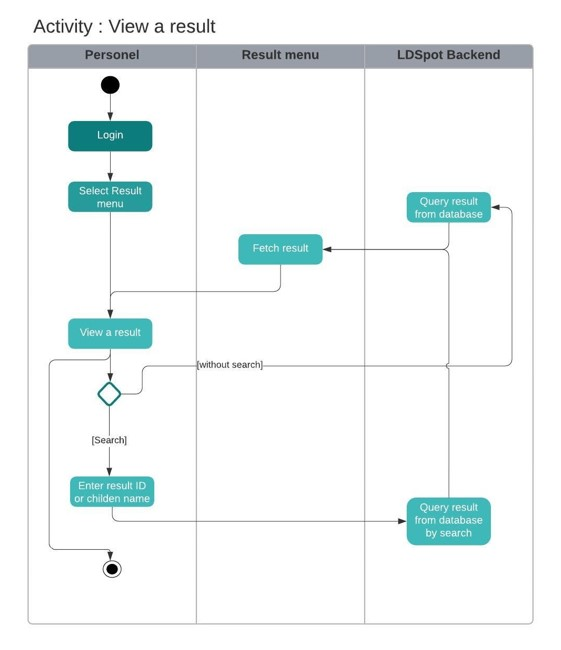
\includegraphics[width=10cm]{./activityresult.jpg}}
      \caption{ภาพ Sequence diagram การดูผลลัพธ์การทดสอบ}\label{fig:activity2}
     \end{figure}
     
  \newpage
     \begin{figure}[!ht]\centering
      \setlength{\fboxrule}{0.2mm} % can define this in the preamble
      \setlength{\fboxsep}{1cm}
      \fbox{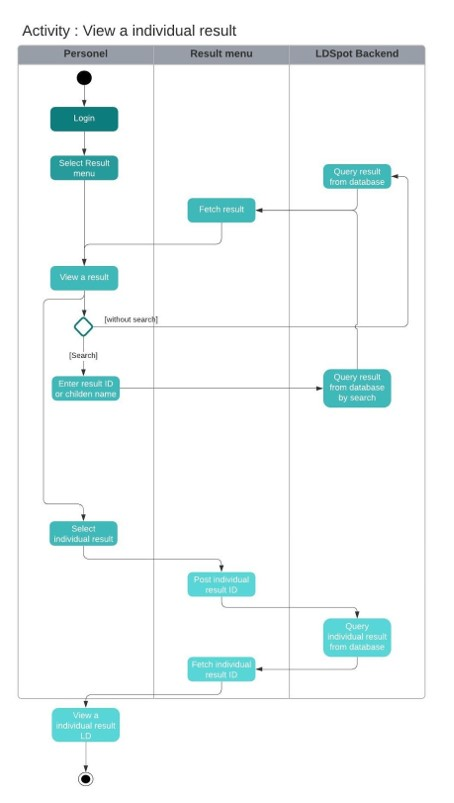
\includegraphics[width=10cm]{./activityresult2.jpg}}
      \caption{ภาพ Sequence diagram การดูผลลัพธ์รายบุคคล}\label{fig:activity22}
     \end{figure}
     \newpage
     \begin{table}[!h]\centering
      \caption{Use case narrative ของการดูผลลัพธ์การทดสอบ}\label{tbl:application1}
      \begin{tabular}{|p{3cm}|p{12cm}|} \hline
      Use Case Name & ผลลัพธ์การทดสอบ \\ \hline
      Goal in Context & เพื่อดูผลลัพธ์การทดสอบของผู้เข้ารับการทดสอบ \\ \hline
      Primary Actor & บุคลากรทางการแพทย์\\ \hline
      Secondary Actor & - \\ \hline
      Precondition & ต้องเข้าสู่ระบบก่อน \\ \hline
      Trigger & บุคลากรทางการแพทย์กดเข้าสู่ระบบดูผลลัพธ์ \\ \hline
      Scenario & \begin{enumerate}
        \item บุคลากรทางการแพทย์กดเข้าสู่ระบบดูผลลัพธ์
        \item ระบบดึงรายชื่อแบบทดสอบมาแสดง
        \item บุคลากรทางการแพทย์สามารถกรอกชื่อหรือรหัสประจำตัวผู้ทำแบบทดสอบเพื่อเป็นการหาได้ 
        \item บุคลากรทางการแพทย์เลือกแบบทดสอบที่ต้องการจะดูผลลัพธ์
        \item ระบบดึงข้อมูลผลลัพธ์แบบทดสอบนั้นมาแสดง 
      \end{enumerate} \\ \hline
      Exception & - \\ \hline
      Post-condition & - \\ \hline
      \end{tabular}
      \end{table}
     \newpage
    \item ดูสถิติรวมของแอปพลิเคชัน
    Sequence diagram นี้อธิบายขั้นตอนการดูสถิติของแอปพลิเคชันโดยผู้ทดสอบจะต้องเข้าสู่ระบบผ่าน ทางแอปพลิเคชัน จากนั้นเข้าส่วนของการดูสถิติ
     แอปพลิเคชันจะทำการดึงข้อมูลสรุปผลต่างๆ จากฐานข้อมูลเช่น ตัวอักษรใดที่คน เขียนผิดมากที่สุด จำนวนคนใช้แอปพลิเคชันเป็นต้นมาแสดงบนพลิเคชัน
    \begin{figure}[!ht]\centering
      \setlength{\fboxrule}{0.2mm} % can define this in the preamble
      \setlength{\fboxsep}{1cm}
      \fbox{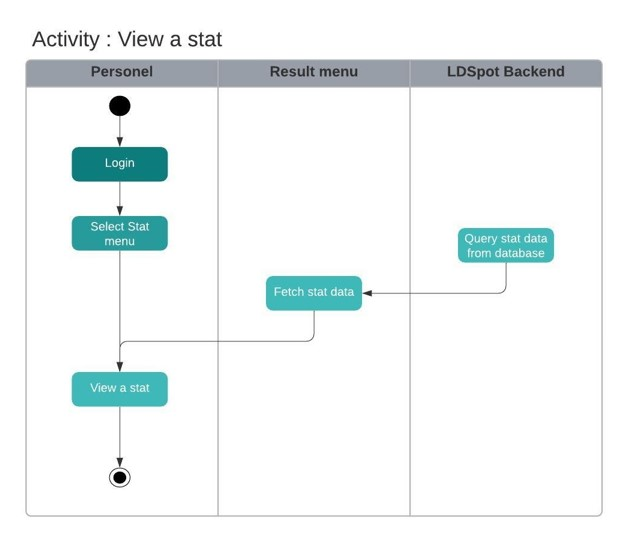
\includegraphics[width=10cm]{./activitystat.jpg}}
      \caption{ภาพ Sequence diagram การดูข้อมูลสถิติในแอปพลิเคชัน}\label{fig:activity3}
     \end{figure}
     \newpage
     \begin{table}[!h]\centering
      \caption{Use case narrative ของการดูข้อมูลสถิติในแอปพลิเคชัน}\label{tbl:application1}
      \begin{tabular}{|p{4cm}|p{10cm}|} \hline
      Use Case Name & ดูข้อมูลสถิติในแอปพลิเคชัน \\ \hline
      Goal in Context & เพื่อดูผลสรุปสถิติของแอปพลิเคชัน \\ \hline
      Primary Actor & บุคลากรทางการแพทย์ \\ \hline
      Secondary Actor & - \\ \hline
      Precondition & ต้องเข้าสู่ระบบก่อน \\ \hline
      Trigger & บุคลากรทางการแพทย์ต้องเข้าสู่หน้าดูสถิติในแอปพลิเคชัน \\ \hline
      Scenario & \begin{enumerate}
        \item บุคลากรทางการแพทย์ต้องเข้าสู่หน้าดูสถิติในแอปพลิเคชัน
        \item ระบบดึงข้อมูลสถิติมาสรุปบนแอปพลิเคชัน 
      \end{enumerate} \\ \hline
      Exception & - \\ \hline
      Post-condition & - \\ \hline
  
      \end{tabular}
      \end{table}
      \newpage
    \item เข้าสู่ระบบ
    Sequence Diagram นี้อธิบายขั้นตอนการเข้าสู่ระบบโดยผู้ทดสอบจะสามารถเข้าสู่ระบบได้ด้วยรหัสของผู้ทดสอบ
    แต่จะสามารถเข้าถึงเมนูทำการทดสอบเพียงเท่านั้น 
    ส่วนบุคลากรทางการแพทย์จะสามารถเข้าสู่ระบบได้ด้วยรหัสของบุคลากรทางการแพทย์ซึ่งจะสามารถเข้าถึงเมนูทั้งหมดภายในแอปพลิเคชันได้
    \begin{figure}[!ht]\centering
      \setlength{\fboxrule}{0.2mm} % can define this in the preamble
      \setlength{\fboxsep}{1cm}
      \fbox{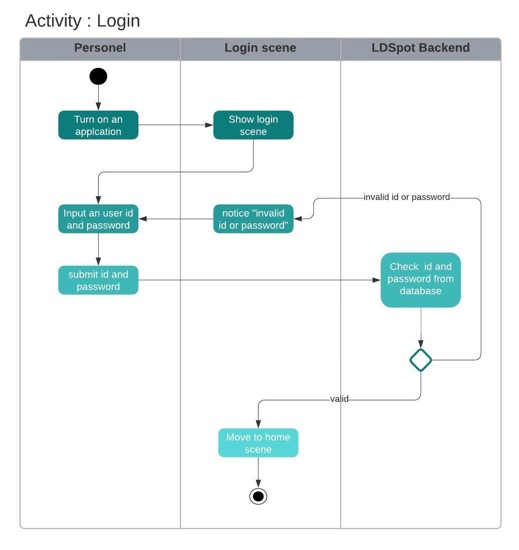
\includegraphics[width=10cm]{./activitylogin.jpg}}
      \caption{ภาพ Sequence diagram การเข้าสู่ระบบ}\label{fig:activity4}
     \end{figure}
     \newpage
     \begin{table}[!h]\centering
      \caption{Use case narrative ของการเข้าสู่ระบบ}\label{tbl:application1}
      \begin{tabular}{|p{4cm}|p{10cm}|} \hline
      Use Case Name & เข้าสู่ระบบ \\ \hline
      Goal in Context & เพื่อเข้าสู่ระบบใช้งานแอปพลิเคชัน \\ \hline
      Primary Actor & บุคลากรทางการแพทย์, ผู้เข้ารับการทำแบบทดสอบ \\ \hline
      Secondary Actor & - \\ \hline
      Precondition & บุคลากรทางการแพทย์หรือผู้เข้ารับการทำแบบทดสอบต้องมีรหัสของตน \\ \hline
      Trigger & บุคลากรทางการแพทย์หรือผู้เข้ารับการทำแบบทดสอบเข้าสู่แอปพลิเคชัน \\ \hline
      Scenario & \begin{enumerate}
        \item บุคลากรทางการแพทย์หรือผู้เข้ารับการทำแบบทดสอบ กรอก ไอดี และรหัสผ่านของตน
        \item จากนั้นกดปุ่มเข้าสู่ระบบ
        \item ระบบนำไอดี และรหัสผ่านไปตรวจสอบในฐานข้อมูลว่าตรงหรือไม่
        \item หากตรงพาเข้าสู่ระบบ และไปยังหน้าเมนูหลัก หากไม่ตรงให้แจ้งเตือนข้อผิดพลาด 
      \end{enumerate} \\ \hline
      Exception & - \\ \hline
      Post-condition & - \\ \hline
  
      \end{tabular}
      \end{table}
      \newpage
      \item แก้ไขผลลัพธ์การทดสอบ
      Sequence Diagram นี้อธิบายขั้นตอนการทำงานการแก้ไขผลลัพธ์แบบทดสอบโดย บุคลากรทางการแพทย์เมื่อเข้าไปในรายละเอียดของแบบทดสอบแล้วจะสามารถกดที่ภาพแบบทดสอบได้เพื่อเปลี่ยนผลลัพธ์แบบทดสอบ
       เช่น ถูก ผิด กลับด้าน โดยระบบนี้มีไว้เพื่อให้บุคลากรทางการแพทย์สามารถตรวจสอบผลลัพธ์การทำนาย และแก้ไขผลลัพธ์การทำนายได้ด้วย
      \begin{figure}[!ht]\centering
        \setlength{\fboxrule}{0.2mm} % can define this in the preamble
        \setlength{\fboxsep}{1cm}
        \fbox{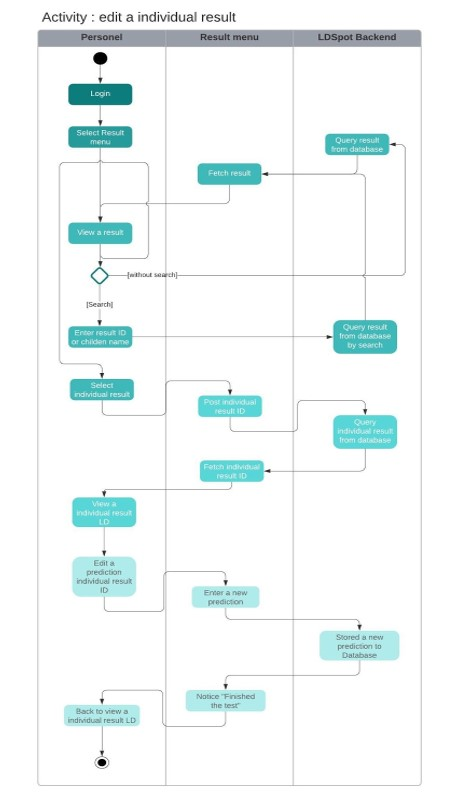
\includegraphics[width=10cm]{./activityedit.jpg}}
        \caption{ภาพ Sequence diagram การแก้ไขผลลัพธ์รายบุคคล}\label{fig:activity5}
       \end{figure}
       \newpage
       \begin{table}[!h]\centering
        \caption{Use case narrative การแก้ไขผลลัพธ์รายบุคคล}\label{tbl:application1}
        \begin{tabular}{|p{4cm}|p{10cm}|} \hline
        Use Case Name & แก้ไขผลลัพธ์การทดสอบ \\ \hline
        Goal in Context & เพื่อให้บุคลากรทางการแพทย์สามารถตรวจสอบ และเปลี่ยนผลลัพธ์การทดสอบได้ \\ \hline
        Primary Actor & บุคลากรทางการแพทย์ \\ \hline
        Secondary Actor & - \\ \hline
        Precondition & บุคลากรทางการแพทย์เข้าดูรายละเอียดของการทำแบบทดสอบ \\ \hline
        Trigger & บุคลากรทางการแพทย์กดแก้ไขผลลัพธ์ที่รูปภาพแบบทดสอบ \\ \hline
        Scenario & \begin{enumerate}
          \item บุคลากรทางการแพทย์เข้าสู่ระบบแอปพลิเคชัน
          \item บุคลากรทางการแพทย์เข้าสู่ส่วนของการดูผลลัพธ์การทดสอบ
          \item บุคลากรทางการแพทย์ทำการเลือกดูผลลัพธ์ของแบบทดสอบใดแบบทดสอบหนึ่ง
          \item บุคลากรทางการแพทย์ทำการกดปุ่มแก้ไขข้างหลังรูปภาพการทำแบบทดสอบ
          \item บุคลากรทางการแพทย์ทำการเลือกผลลัพธ์ใหม่สำหรับภาพนั้น จากนั้นกดยืนยัน
          \item ระบบนำผลลัพธ์ไปแก้ไขภายในฐานข้อมูล จากนั้นทำการแสดงรายละเอียดของแบบทดสอบนั้นใหม่ 
        \end{enumerate} \\ \hline
        Exception & - \\ \hline
        Post-condition & - \\ \hline
    
        \end{tabular}
        \end{table}
        \newpage
        \item สมัครสมาชิก
        Sequence Diagram นี้อธิบายขั้นตอนการทำงานของระบบการสมัครสมาชิก โดยจะมีอยู่สองรูปแบบด้วยกัน คือนักเรียน และบุคลากรทางการแพทย์ 
        โดยข้อมูลที่ต้องกรอกจะเป็นข้อมูลพื้นฐานได้แก่ ไอดี รหัสผ่านชื่อ นามสกุล แต่ในส่วนของนักเรียน จะมีการกรอกข้อมูลรหัสประจำตัว วันเกิด และระดับชั้นการศึกษาเพิ่มขึ้นมา
        \newpage
        \begin{figure}[!ht]\centering
          \setlength{\fboxrule}{0.2mm} % can define this in the preamble
          \setlength{\fboxsep}{1cm}
          \fbox{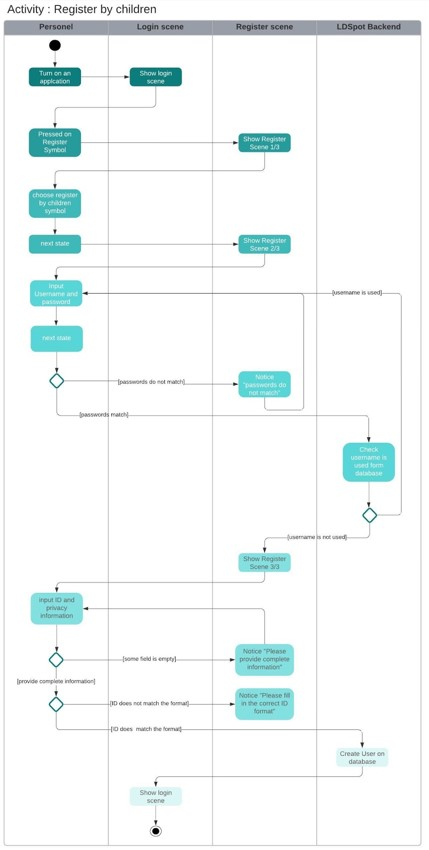
\includegraphics[width=10cm]{./activityregisterchildren.jpg}}
          \caption{ภาพ Sequence diagram การสมัครสมาชิกแบบนักเรียน}\label{fig:activity6}
         \end{figure}
         \newpage
         \begin{figure}[!ht]\centering
          \setlength{\fboxrule}{0.2mm} % can define this in the preamble
          \setlength{\fboxsep}{1cm}
          \fbox{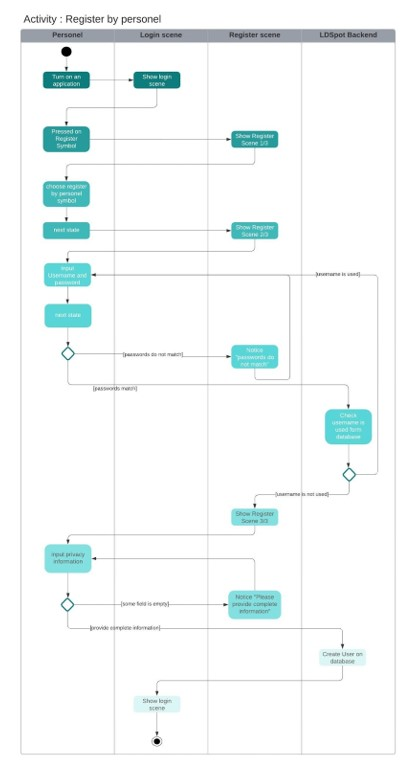
\includegraphics[width=10cm]{./activityregisterperson.jpg}}
          \caption{ภาพ Sequence diagram การสมัครสมาชิกแบบบุคลากรทางการแพทย์}\label{fig:activity7}
         \end{figure}
         \newpage
         \begin{table}[!h]\centering
          \caption{Use case narrative ของการสมัครสมาชิก}\label{tbl:register}
          \begin{tabular}{|p{3cm}|p{12cm}|} \hline
          Use Case Name & สมัครสมาชิก \\ \hline
          Goal in Context & เพื่อให้บุคลากรทางการแพทย์ และผู้เข้ารับการทำแบบทดสอบสามารถสมัครรหัสสมาชิกของตนได้ \\ \hline
          Primary Actor & บุคลากรทางการแพทย์, ผู้เข้ารับการทำแบบทดสอบ  \\ \hline
          Secondary Actor & - \\ \hline
          Precondition & บุคลากรทางการแพทย์หรือผู้เข้ารับการทำแบบทดสอบเข้าสู่แอปพลิเคชัน \\ \hline
          Trigger & บุคลากรทางการแพทย์หรือผู้เข้ารับการทำแบบทดสอบกดสมัครสมาชิกภายในหน้าเข้าสู่ระบบ \\ \hline
          Scenario & \begin{enumerate}
            \item บุคลากรทางการแพทย์หรือผู้เข้ารับการทำแบบทดสอบเข้าสู่ระบบสมัครสมาชิก
            \item บุคลากรทางการแพทย์หรือผู้เข้ารับการทำแบบทดสอบเลือกประเภทการสมัครสมาชิกของตน
            \item บุคลากรทางการพทย์หรือผู้เข้ารับการทำแบบทดสอบทำการกรอกข้อมูลจากนั้นกดสมัครสมาชิก
            \item ระบบนำข้อมูลไปเก็บในฐานข้อมูล
           
          \end{enumerate} \\ \hline
          Exception & - \\ \hline
          Post-condition & - \\ \hline
      
          \end{tabular}
          \end{table}
  \end{itemize}

\newpage
  \section{Model architecture}
  \begin{itemize}
    \item Convolutional Layer
    \begin{figure}[!ht]\centering
      \setlength{\fboxrule}{0.2mm} % can define this in the preamble
      \setlength{\fboxsep}{1cm}
      \fbox{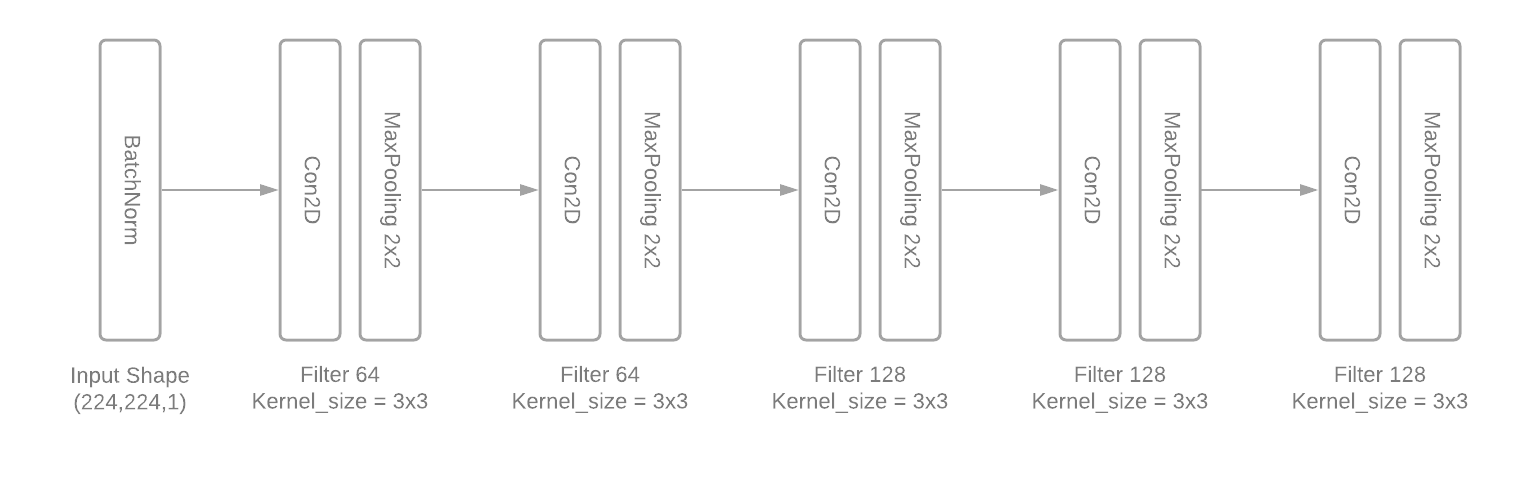
\includegraphics[width=13cm]{./convalphabetmodel.png}}
      \caption{Convolutional Layer สำหรับโมเดลตัวอักษร}\label{fig:convolutionallayer}
     \end{figure}
     \begin{figure}[!ht]\centering
      \setlength{\fboxrule}{0.2mm} % can define this in the preamble
      \setlength{\fboxsep}{1cm}
      \fbox{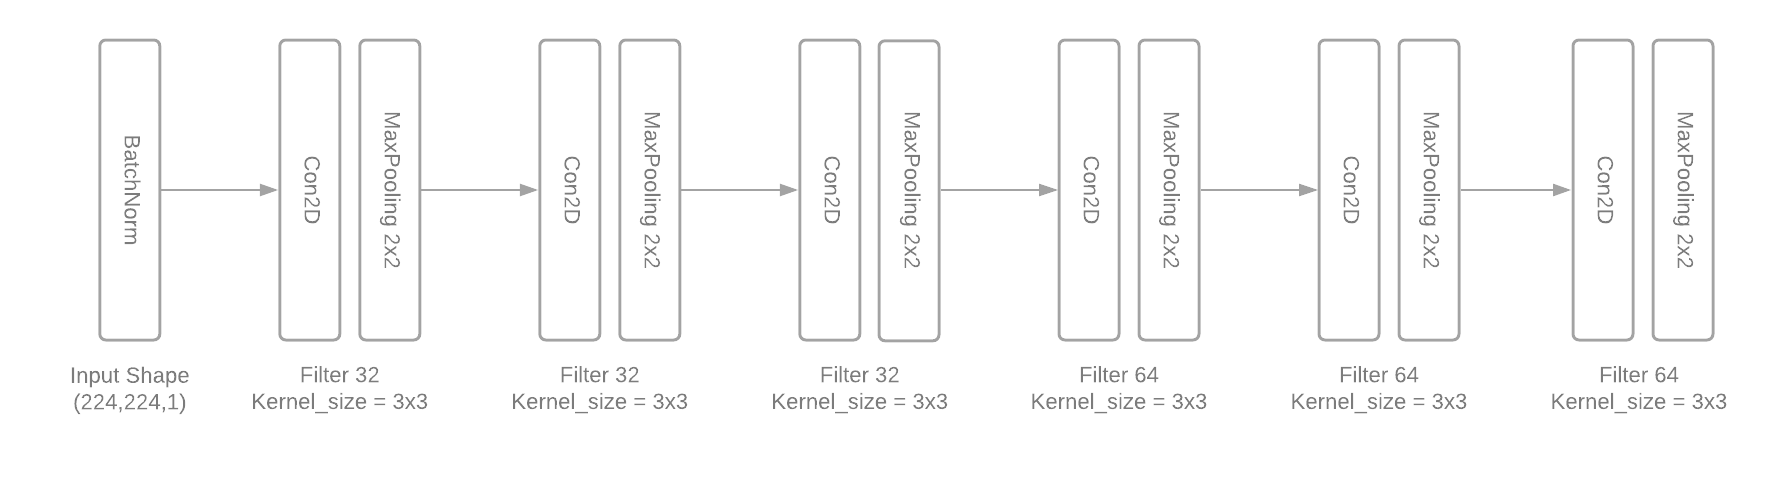
\includegraphics[width=13cm]{./convvowelmodel.png}}
      \caption{Convolutional Layer สำหรับโมเดลสระ}\label{fig:convolutionallayer}
     \end{figure}
  
  \item BatchNorm ที่อยู่ใน Input Layer ทำให้มันสามารถปรับ Shift หรือ Scale ระหว่างเทรน ของ Activation  
  ที่อยู่ภายใน Hidden layer มีขนาดเหมาะสมไม่เล็กไม่ใหญ่เกินไป โดยอ้างอิงจากค่าเฉลี่ย และค่าเบี่ยงเบนมาตรฐาน และช่วยทำให้แต่ละ Layer สามารถเรียนรู้ของตัวเองเป็นอิสระมากขึ้น
  \item Con2D หรือ Convolutional layer รวมกับ MaxPooling ที่เป็น Pooling layer เป็นการทำ Feature Extraction ออกจากรูปภาพเพื่อให้สามารถหาลักษณะเฉพาะของวัตถุได้ และสามารถจำแนกได้
  \newpage
  \item Model สำหรับตัวอักษร 
  \begin{figure}[!ht]\centering
    \setlength{\fboxrule}{0.2mm} % can define this in the preamble
    \setlength{\fboxsep}{1cm}
    \fbox{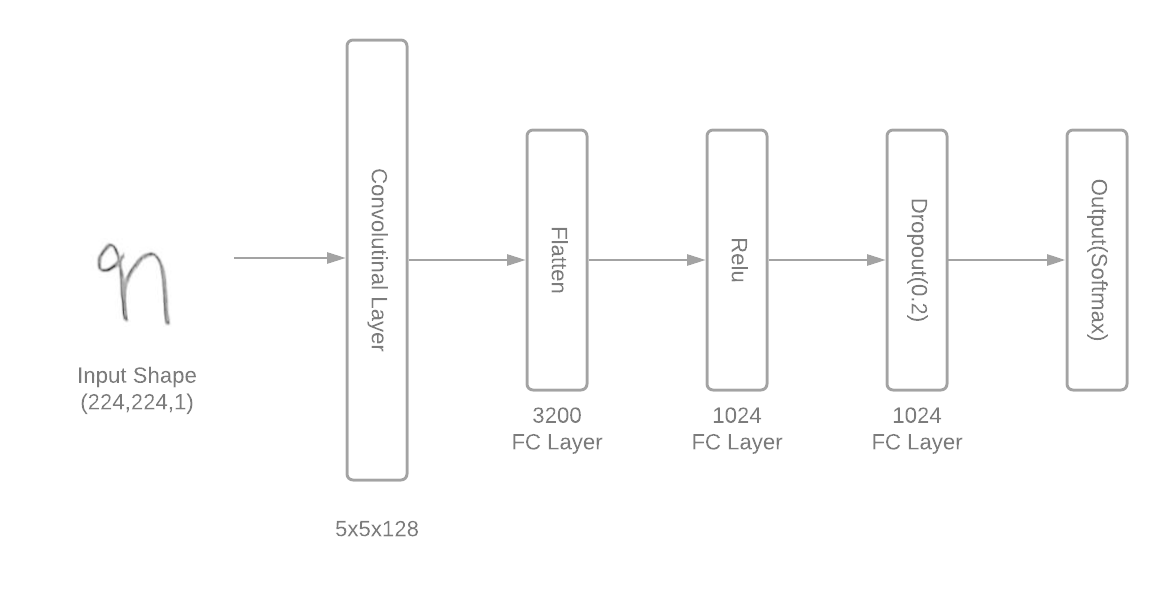
\includegraphics[width=13cm]{./alphabetmodel.png}}
    \caption{โมเดลสำหรับตัวอักษร}\label{fig:modelarchitecture}
   \end{figure}
  \item Model สำหรับสระ
  \begin{figure}[!ht]\centering
    \setlength{\fboxrule}{0.2mm} % can define this in the preamble
    \setlength{\fboxsep}{1cm}
    \fbox{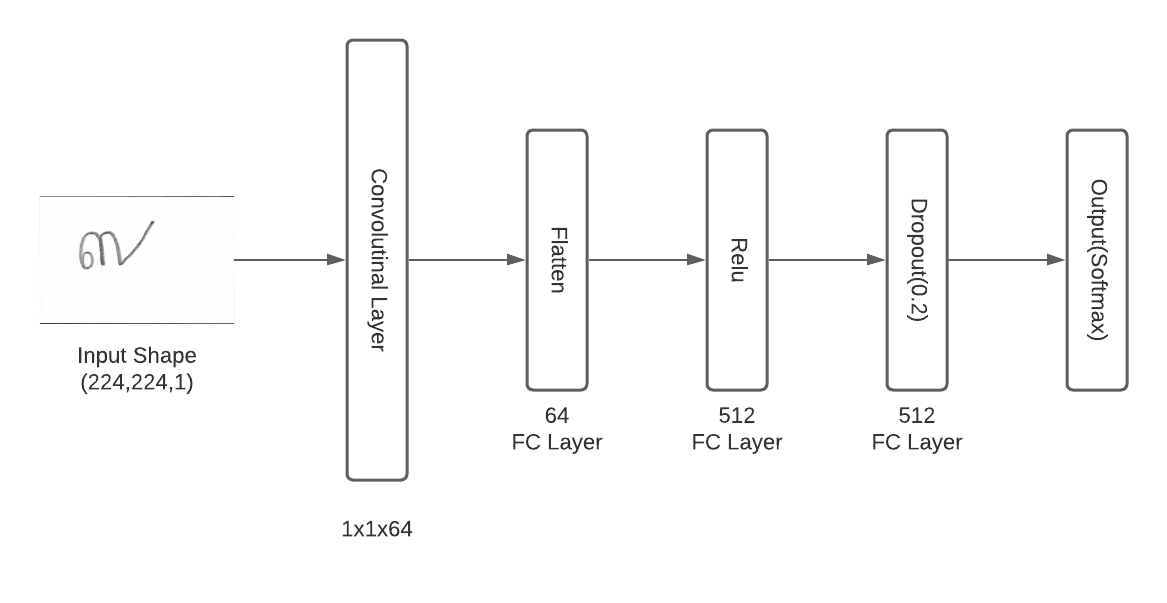
\includegraphics[width=13cm]{./vowelmodel.png}}
    \caption{โมเดลสำหรับตัวอักษร}\label{fig:modelarchitecturevowel}
   \end{figure}
  \end{itemize}
\newpage
\section{User Interface Design}
\begin{itemize}
  \item หน้าต่างเข้าสู่ระบบ
  \begin{figure}[!ht]\centering
    \setlength{\fboxrule}{0.2mm} % can define this in the preamble
    \setlength{\fboxsep}{1cm}
    \fbox{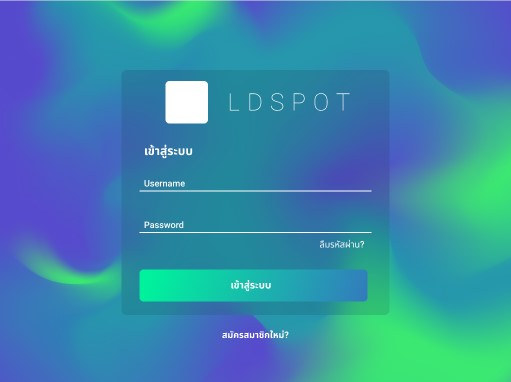
\includegraphics[width=10cm]{./login.jpg}}
    \caption{ภาพการออกแบบหน้าเข้าสู่ระบบ}\label{fig:system}
  \end{figure}
  \item หน้ากรอกข้อมูลสำหรับเริ่มทำแบบทดสอบ
  \begin{figure}[!ht]\centering
    \setlength{\fboxrule}{0.2mm} % can define this in the preamble
    \setlength{\fboxsep}{1cm}
    \fbox{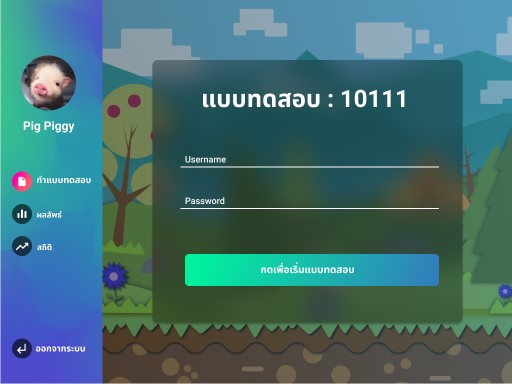
\includegraphics[width=10cm]{./home.jpg}}
    \caption{ภาพการออกแบบหน้ากรอกข้อมูลสำหรับเริ่มทำแบบทดสอบ}\label{fig:system}
  \end{figure}
  \newpage
  \item หน้าแรกของเกมในการทำแบบทดสอบ
  \begin{figure}[!ht]\centering
    \setlength{\fboxrule}{0.2mm} % can define this in the preamble
    \setlength{\fboxsep}{1cm}
    \fbox{
\includegraphics[width=10cm]{./stage1.jpg}}
    \caption{ภาพการออกแบบหน้าการทำแบบทดสอบด่านแรก}\label{fig:system}
  \end{figure}
  \item หน้าสองของเกมในการทำแบบทดสอบ
  \begin{figure}[!ht]\centering
    \setlength{\fboxrule}{0.2mm} % can define this in the preamble
    \setlength{\fboxsep}{1cm}
    \fbox{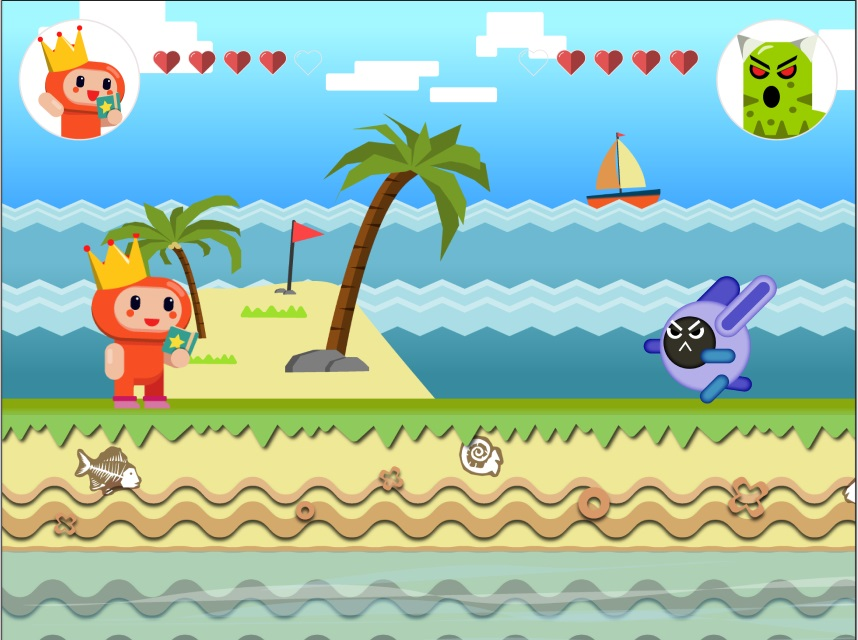
\includegraphics[width=10cm]{./stage2.jpg}}
    \caption{ภาพการออกแบบหน้าการทำแบบทดสอบด่านสอง}\label{fig:system}
  \end{figure}
  \newpage
  \item หน้าสุดท้ายของเกมในการทำแบบทดสอบ
  \begin{figure}[!ht]\centering
    \setlength{\fboxrule}{0.2mm} % can define this in the preamble
    \setlength{\fboxsep}{1cm}
    \fbox{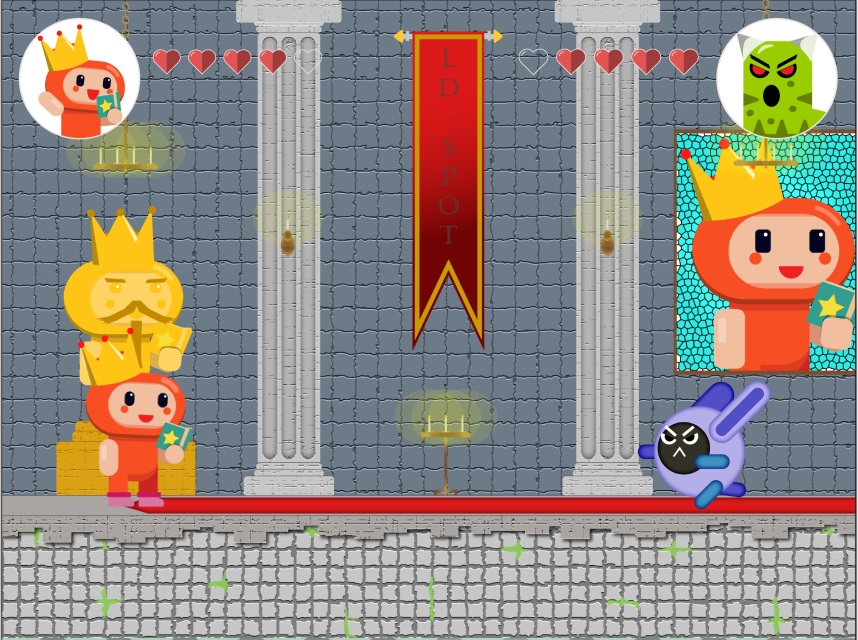
\includegraphics[width=10cm]{./stage3.jpg}}
    \caption{ภาพการออกแบบหน้าการทำแบบทดสอบด่านสาม}\label{fig:system}
  \end{figure}
  \item หน้าปุ่มกดข้ามตัวอักษร สระ หรือคำสะกด
  \begin{figure}[!ht]\centering
    \setlength{\fboxrule}{0.2mm} % can define this in the preamble
    \setlength{\fboxsep}{1cm}
    \fbox{
\includegraphics[width=10cm]{./stage1inputSkip.jpg}}
    \caption{ภาพการออกแบบหน้าการกดข้ามการเขียนตัวอักษร สระ และคำสะกด}\label{fig:system}
  \end{figure}
  \newpage
  \item หน้าต่างสำหรับเขียนตัวอักษร สระ และคำสะกด
  \begin{figure}[!ht]\centering
    \setlength{\fboxrule}{0.2mm} % can define this in the preamble
    \setlength{\fboxsep}{1cm}
    \fbox{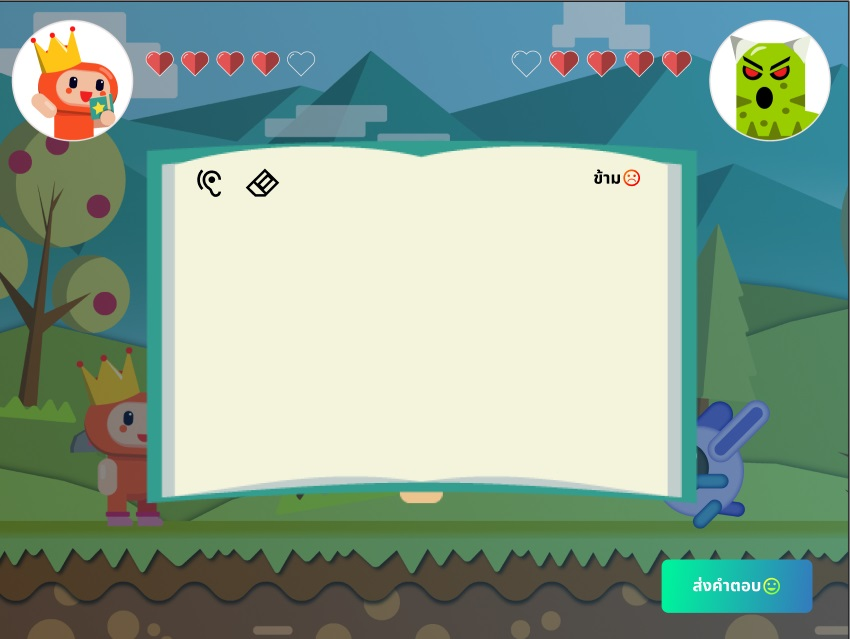
\includegraphics[width=10cm]{./stage1input.jpg}}
    \caption{ภาพการออกแบบหน้าเขียนตัวอักษร สระ และคำสะกด}\label{fig:system}
  \end{figure}
  \begin{figure}[!ht]\centering
    \setlength{\fboxrule}{0.2mm} % can define this in the preamble
    \setlength{\fboxsep}{1cm}
    \fbox{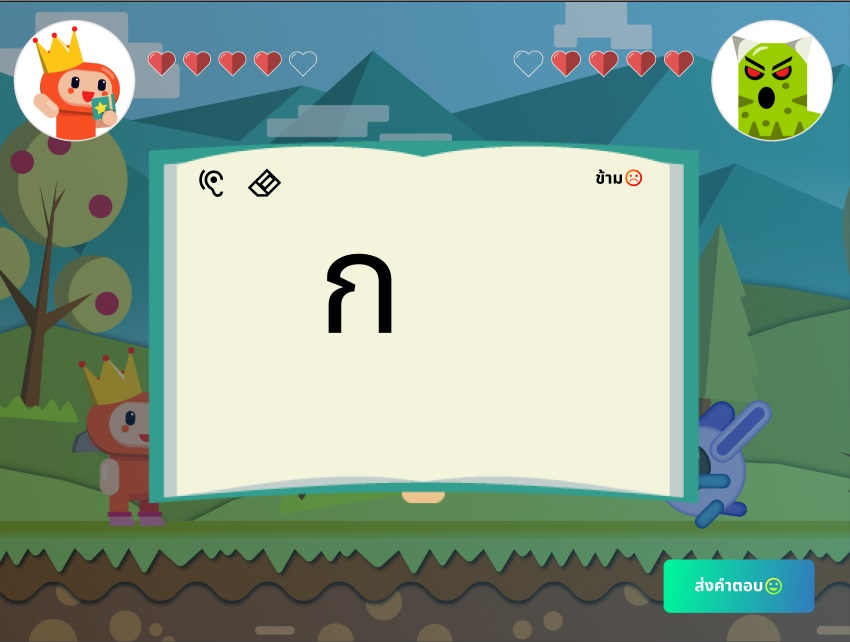
\includegraphics[width=10cm]{./stage1input2.jpg}}
    \caption{ภาพการออกแบบหน้าเขียนตัวอักษร สระ และคำสะกด}\label{fig:system}
  \end{figure}
  \newpage
  \item หน้าเกมสำหรับจบแบบทดสอบ
  \begin{figure}[!ht]\centering
    \setlength{\fboxrule}{0.2mm} % can define this in the preamble
    \setlength{\fboxsep}{1cm}
    \fbox{
\includegraphics[width=10cm]{./endGame.jpg}}
    \caption{ภาพการออกแบบหน้าจบการทดสอบ}\label{fig:system}
  \end{figure}
  \item หน้าดูผลลัพธ์การทดสอบ
    \begin{figure}[!ht]\centering
      \setlength{\fboxrule}{0.2mm} % can define this in the preamble
      \setlength{\fboxsep}{1cm}
      \fbox{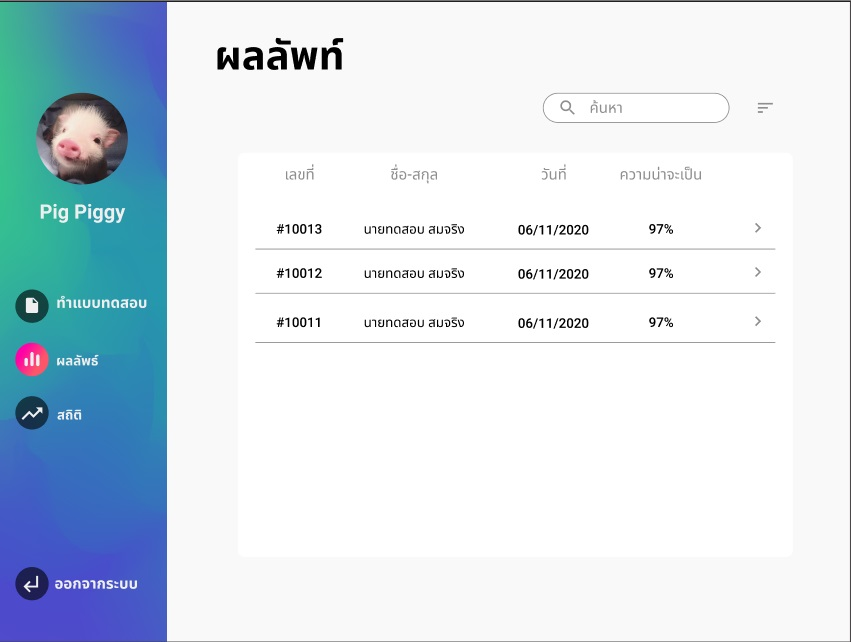
\includegraphics[width=10cm]{./result.jpg}}
      \caption{ภาพออกแบบหน้าดูผลลัพธ์การทดสอบ}\label{fig:system}
    \end{figure}
  \newpage
  \item หน้าดูข้อมูลสถิติภายในแอปพลิเคชัน
    \begin{figure}[!ht]\centering
      \setlength{\fboxrule}{0.2mm} % can define this in the preamble
      \setlength{\fboxsep}{1cm}
      \fbox{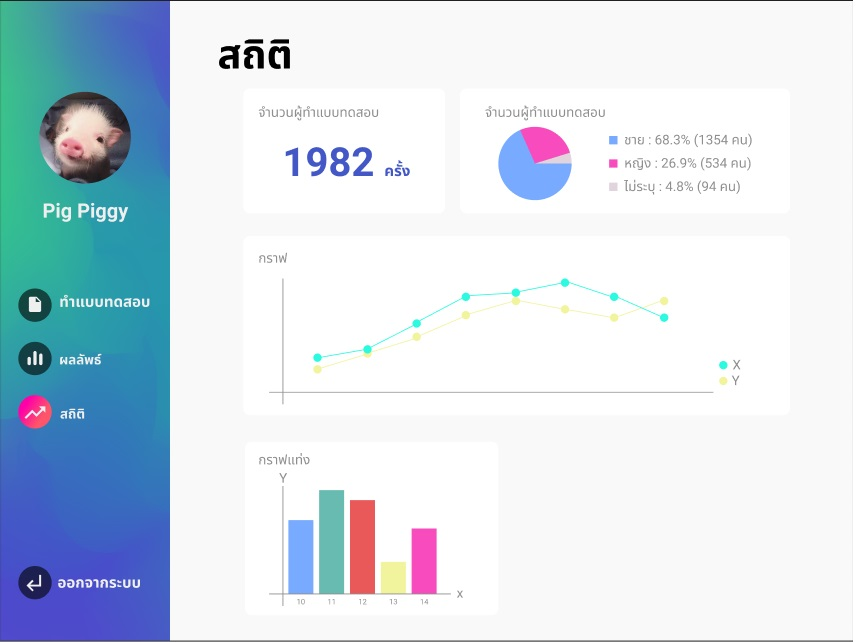
\includegraphics[width=10cm]{./stat.jpg}}
      \caption{ภาพการออกแบบหน้าดูสถิติภายในแอปพลิเคชัน}\label{fig:system}
        
  \end{figure}
\end{itemize}
\newpage
\section{การเก็บข้อมูลภาพลายมือเด็ก}
การเก็บรวมรวมข้อมูลของภาพลายมือเด็ก คณะผู้จัดทำได้ทำการรวมรวมรูปภาพการทำแบบทดสอบโดยเขียนพยัญชนะ สระ และคำสะกด 
จากนักเรียนระดับชั้นประถมศึกษาตั้งแต่ประถมศึกษาปีที่หนึ่งถึงประถมศึกษาปีที่สาม โดยคาดว่าจะมีเด็กเข้าร่วมทำแบบทดสอบประมาณ 1,000 
คนโดยประมาณ ซึ่งภาพลายมือเด็กที่เขียนถูกต้องจะถูกนำมาใช้ในการเรียนรู้ของตัวโมเดล โดยตัวอย่างแบบทดสอบมีดังนี้
\begin{figure}[!ht]\centering
  \setlength{\fboxrule}{0.2mm} % can define this in the preamble
  \setlength{\fboxsep}{1cm}
  \fbox{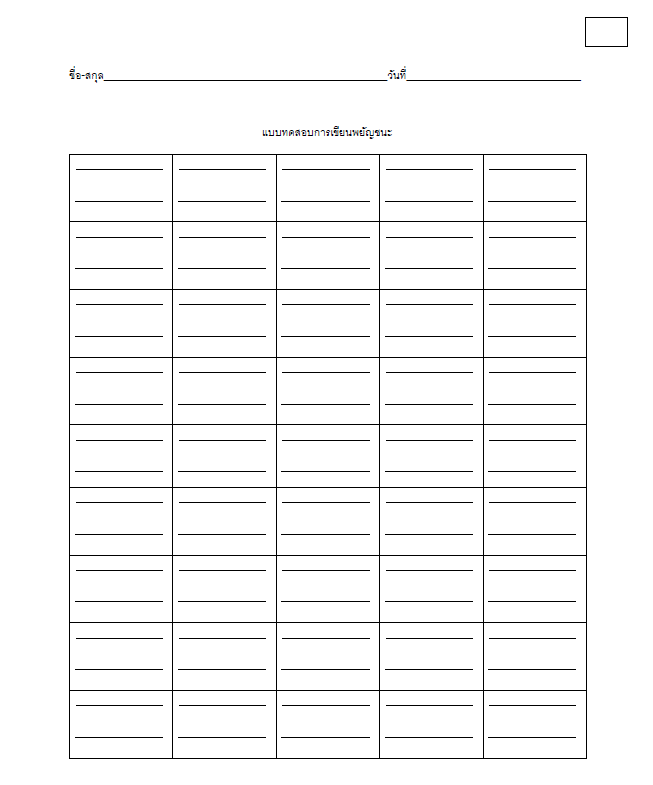
\includegraphics[width=10cm,height=10cm]{./พยัญชนะ.png}}
  \caption{ภาพแบบทดสอบที่ใช้เก็บลายมือตัวอักษรเด็ก}\label{fig:system}
    
\end{figure}
\newpage
\begin{figure}[!ht]\centering
  \setlength{\fboxrule}{0.2mm} % can define this in the preamble
  \setlength{\fboxsep}{1cm}
  \fbox{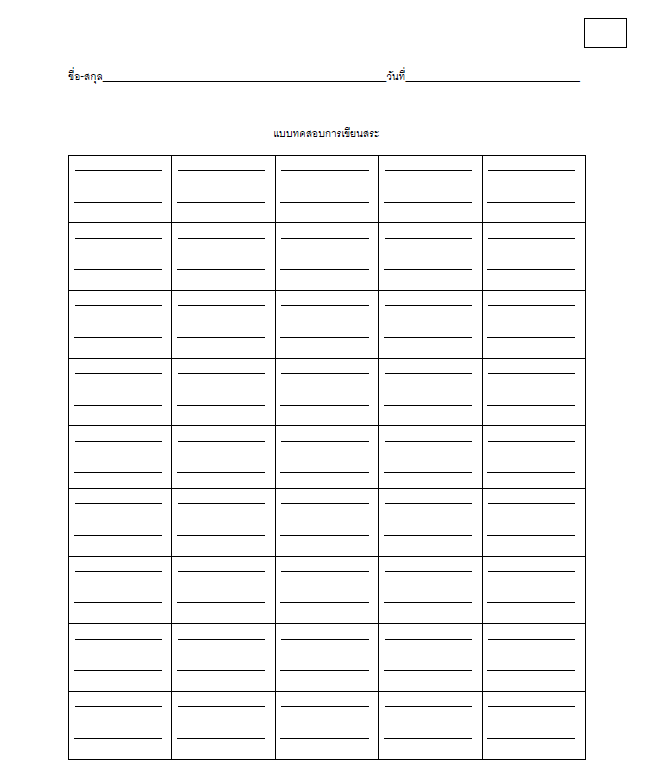
\includegraphics[width=10cm,height=10cm]{./สระ.png}}
  \caption{ภาพแบบทดสอบที่ใช้เก็บลายมือสระเด็ก}\label{fig:system}
    
\end{figure}
\begin{figure}[!ht]\centering
  \setlength{\fboxrule}{0.2mm} % can define this in the preamble
  \setlength{\fboxsep}{1cm}
  \fbox{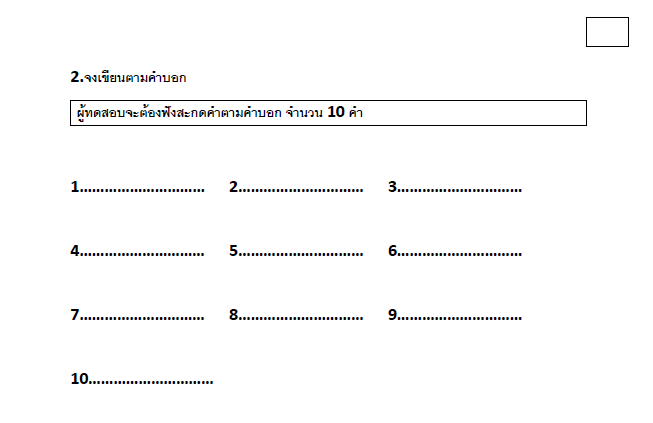
\includegraphics[width=10cm]{./คำสะกด.png}}
  \caption{ภาพแบบทดสอบที่ใช้เก็บลายมือคำสะกดเด็ก}\label{fig:system}
    
\end{figure}
\newpage

\section{แผนการประเมินประสิทธิภาพของแอปพลิเคชัน}
คณะผู้จัดทำจะนำตัวแอปพลิเคชันไปวัดผลที่ หน่วยตรวจโรคจิตเวชเด็ก และวัยรุ่น ภาควิชาจิตเวชศาสตร์ คณะแพทยศาสตร์ศิริราชพยาบาล  ซึ่งบุคลากรจะนำตัวแอปพลิเคชันไปทดสอบกับเด็ก เพื่อสังเกตผลลัพธ์ว่า แอปพลิเคชันกับบุคลากรนั้น สามารถจำแนกประเภทอาการของเด็กออกมาได้ตรงกันหรือไม่ 

\chapter{ผลการวิจัย และอภิปรายผล}
\section{Application Interface}
\begin{itemize}
  \item หน้าต่างเข้าสู่ระบบ
  \begin{figure}[!ht]\centering
    \setlength{\fboxrule}{0.2mm} % can define this in the preamble
    \setlength{\fboxsep}{1cm}
    \fbox{\includegraphics[width=14cm]{./loginstep.png}}
    \caption{วิธีการใช้งานหน้าเข้าสู่ระบบ}\label{fig:system}
  \end{figure}
  หากใส่ชื่อผู้ใช้ และรหัสผ่านถูกต้องที่อ้างอิงจากฐานข้อมูลเท่านั้น จึงสามารถเข้าใช้งานได้
  \begin{enumerate}
    \item ส่วนในการกรอกชื่อผู้ใช้ (username) และรหัสผ่าน (password)
    \item ปุ่มสำหรับการเข้าสู่ระบบ
    \item ปุ่มสำหรับการสมัครสมาชิก โดยแตะเพื่อเปลี่ยนไปยังส่วนสมัครสมาชิก
  \end{enumerate} 
  \newpage
  \item หน้าสมัครสมาชิก(ประเภท)
  \begin{figure}[!ht]\centering
    \setlength{\fboxrule}{0.2mm} % can define this in the preamble
    \setlength{\fboxsep}{1cm}
    \fbox{\includegraphics[width=14cm]{./howtouse2.jpg}}
    \caption{หน้าเลือกรูปแบบการสมัครสมาชิกของ แอลดีสปอต}\label{fig:register}
  \end{figure}
  \begin{enumerate}
    \item ส่วนที่บอกว่าอยู่ขั้นใดในการสมัครสมาชิก
    \item ส่วนที่เลือกประเภทของการสมัครสมาชิก
    \item ปุ่มถัดไป เพื่อลิงค์ไปยังขั้นตอนถัดไป
  \end{enumerate}
  \newpage
  \item หน้าสมัครสมาชิก(สร้างบัญชี)
  \begin{figure}[!ht]\centering
    \setlength{\fboxrule}{0.2mm} % can define this in the preamble
    \setlength{\fboxsep}{1cm}
    \fbox{\includegraphics[width=14cm]{./howtouse3.jpg}}
    \caption{หน้าสมัครสมาชิกของ แอลดีสปอต}\label{fig:register2}
  \end{figure}
  \begin{enumerate}
    \item ส่วนที่กรอก ชื่อ รหัสผ่าน และยืนยันรหัสผ่าน
    \item ปุ่มถัดไป เพื่อลิงค์ไปยังขั้นตอนถัดไป
  \end{enumerate}
  \newpage
  \item หน้าสมัครสมาชิก(ข้อมูลส่วนตัว)
  หากกรอกทุกอย่างถูกต้องสมบูรณ์ ถึงสามารถสมัครสมาชิกได้
  \begin{figure}[!ht]\centering
    \setlength{\fboxrule}{0.2mm} % can define this in the preamble
    \setlength{\fboxsep}{1cm}
    \fbox{\includegraphics[width=14cm]{./howtouse4.jpg}}
    \caption{หน้าสมัครสมาชิกของ แอลดีสปอต}\label{fig:register3}
  \end{figure}
  \begin{enumerate}
    \item ส่วนที่กรอกข้อมูลส่วนตัว ไอดีของนักเรียน (หากเลือกสมัครประเภทนักเรียนสามารถมองเห็นช่องนี้ได้) ชื่อ นามสกุล วันเกิด และระดับชั้นปีที่กำลังศึกษา
    \item ปุ่มสมัครสมาชิก
  \end{enumerate}
  \newpage
 

  \item หน้าหลัก (แบบทดสอบ)
  \begin{figure}[!ht]\centering
    \setlength{\fboxrule}{0.2mm} % can define this in the preamble
    \setlength{\fboxsep}{1cm}
    \fbox{\includegraphics[width=14cm]{./teststep.png}}
    \caption{หน้าหลัก (แบบทดสอบ) แอลดีสปอต}\label{fig:system}
  \end{figure}
  \begin{enumerate}
    \item ส่วนที่แสดงข้อมูลของผู้ใช้ (หากเป็นรหัสนักเรียน ข้อมูลถูกแสดงไว้ตามข้อมูลที่สมัคร)
    \item ปุ่มเลือกระดับแบบทดสอบ และปุ่มเริ่มทำแบบทดสอบ (ระดับแบบทดสอบมีไว้เพื่อ การทดสอบที่มีความยากง่ายต่างกัน)
  \end{enumerate}
  \newpage
  \item หน้าหลัก (ผลลัพธ์)
  \begin{figure}[!ht]\centering
    \setlength{\fboxrule}{0.2mm} % can define this in the preamble
    \setlength{\fboxsep}{1cm}
    \fbox{\includegraphics[width=14cm]{./paginationstep2.png}}
    \caption{หน้าหลัก (ผลลัพธ์) แอลดีสปอต}\label{fig:system}
  \end{figure}
  \begin{enumerate}
    \item ปุ่มค้นหา
    \item ส่วนที่แสดงข้อมูลของผู้ที่ทำแบบทดสอบ (เลขประจำตัว ชื่อ วันที่ทำ ความน่าจะเป็น)
    \item ส่วนที่กดเข้าไปดูข้อมูลเพิ่มเติมของการทำทดสอบนั้น
    \item เลือกหน้าผลการทดสอบอื่นๆ
  \end{enumerate}
  \newpage
  \item หน้าหลัก (ผลลัพธ์รายละเอียด)
  \begin{figure}[!ht]\centering
    \setlength{\fboxrule}{0.2mm} % can define this in the preamble
    \setlength{\fboxsep}{1cm}
    \fbox{\includegraphics[width=14cm]{./resultstep.png}}
    \caption{หน้าหลัก (ผลลัพธ์รายละเอียด) แอลดีสปอต}\label{fig:system}
  \end{figure}
  \begin{enumerate}
    \item ส่วนที่แสดงผลว่าเขียนถูกเขียนผิดของแต่ละประเภท
    \item ส่วนที่ดูว่ารูปภาพของแต่ละอักษรที่เขียน และความน่าจะเป็นที่ความถูกต้องของตัวอักษรนั้นๆ
    \item ส่วนที่สามารถแก้ไขได้ว่าตัวอักษรนั้นทำนายถูกหรือผิด
  \end{enumerate}
  \newpage
  \item หน้าหลัก (ผลลัพธ์รายบุคคล)
  \begin{figure}[!ht]\centering
    \setlength{\fboxrule}{0.2mm} % can define this in the preamble
    \setlength{\fboxsep}{1cm}
    \fbox{\includegraphics[width=14cm]{./paginationstep.png}}
    \caption{หน้าหลัก (ผลลัพธ์รายบุคคล) แอลดีสปอต}\label{fig:endgame}
  \end{figure}
  \begin{enumerate}
    \item ช่องสำหรับการค้นหาโดยอ้างอิงจากชื่อหรือเลขที่ประจำตัว (HN)
    \item ส่วนสำหรับการแสดงข้อมูลของเด็กทำแบบทดสอบ โดยแสดงเลขที่ประจำตัว และชื่อ สกุล
    หน้าบุคคล (กราฟ)
  \end{enumerate}
  \newpage
  \item หน้าหลัก (ผลลัพธ์รายบุคคลสถิติ)
  \begin{figure}[!ht]\centering
    \setlength{\fboxrule}{0.2mm} % can define this in the preamble
    \setlength{\fboxsep}{1cm}
    \fbox{\includegraphics[width=14cm]{./graphstep.png}}
    \caption{หน้าหลัก (ผลลัพธ์รายบุคคลสถิติ) แอลดีสปอต}\label{fig:endgame}
  \end{figure}
  \begin{enumerate}
    \item ปุ่มสำหรับดูรายละเอียดของกราฟของผู้ใช้
    \item ปุ่มสำหรับดูรายละเอียดของแบบทดสอบของผู้ใช้
    \item ส่วนกราฟแสดงรายละเอียดจำนวนคำคือ จำนวนที่เขียนถูก เขียนผิด เขียนกลับด้าน และรอแพทย์ตัดสินใจที่พบในแต่ละรอบของการทำแบบทดสอบ
  \end{enumerate}
  \newpage
  \item หน้าหลัก (ผลลัพธ์รายบุคคลแบบทดสอบ)
  \begin{figure}[!ht]\centering
    \setlength{\fboxrule}{0.2mm} % can define this in the preamble
    \setlength{\fboxsep}{1cm}
    \fbox{\includegraphics[width=14cm]{./individualresultstep.png}}
    \caption{หน้าหลัก (ผลลัพธ์รายบุคคลแบบทดสอบ) แอลดีสปอต}\label{fig:endgame}
  \end{figure}
  \begin{enumerate}
    \item ปุ่มสำหรับดูรายละเอียดของกราฟของผู้ใช้
    \item ปุ่มสำหรับดูรายละเอียดของแบบทดสอบของผู้ใช้
    \item ส่วนแสดงรายระเอียดของการทดสอบที่แสดงรอบที่ทำ เลขที่ รวมถึงวันที่
    \item ปุ่มสำหรับการเข้าไปดูส่วนของรายละเอียดของการทำแบบทดสอบ
  \end{enumerate}
  \newpage
  \item หน้าแบบทดสอบ โดยแบบทดสอบจะมีการแบ่งเป็น 3 ด่านโดยมีการใช้ พยัญชนะ สระ คำสะกดเป็นตัวแบ่ง และแต่ละด้านมีพื้นหลังที่ต่างกัน
    \begin{figure}[!ht]\centering
      \setlength{\fboxrule}{0.2mm} % can define this in the preamble
      \setlength{\fboxsep}{1cm}
      \fbox{\includegraphics[width=14cm]{./writestep.png}}
      \caption{หน้าแบบทดสอบ แอลดีสปอต}\label{fig:result}
    \end{figure}
    \begin{enumerate}
      \item ปุ่มกดเพื่อฟังเสียงตัวอักษรว่าต้องเขียนตัวใด
      \item ปุ่มลบ
      \item พื้นที่เขียนตัวอักษร สระ คำ จากที่เราได้ยิน
      \item ปุ่มส่งคำตอบ
    \end{enumerate}
    \newpage

  \item หน้าดูข้อมูลสถิติภายในแอปพลิเคชัน
    \begin{figure}[!ht]\centering
      \setlength{\fboxrule}{0.2mm} % can define this in the preamble
      \setlength{\fboxsep}{1cm}
      \fbox{\includegraphics[width=14cm]{./statstep.png}}
      \caption{หน้าดูข้อมูลสถิติภายในแอปพลิเคชันของ แอลดีสปอต}\label{fig:statapplication}
  \end{figure}
  \begin{enumerate}
    \item ส่วนที่แสดงลายระเอียดของกราฟ ตัวอย่างกราฟเช่น จำนวนเพศชายเพศหญิงที่ใช้แอปพลิเคชันทั้งหมด พยัญชนะที่พบว่าผิดบ่อยมากที่สุด 3 ตัว รวมทั้งของสระ และคำ
  \end{enumerate}
\end{itemize}
\newpage
\section{การนำข้อมูลลายมือเด็กมาใช้}
จากการที่คณะผู้จัดทำไปเก็บภาพลายมือเด็กจากโรงเรียนทั้งสิ้นสองโรงเรียน ได้แก่ โรงเรียนวัดไทร และ โรงเรียนดวงวิภา เป็นจำนวนทั้งสิ้น 300 คนแล้วนำมาสแกนรูปภาพ และนำรูปภาพเหล่านั้นไปผ่านโปรแกรมตัดตัวอักษรที่ได้พัฒนาขึ้น
เพื่อที่จะภาพตัวอักษรเหล่านั้นไปใช้ในการให้โมเดลเรียนรู้   
\begin{figure}[!ht]\centering
  \setlength{\fboxrule}{0.2mm} % can define this in the preamble
  \setlength{\fboxsep}{1cm}
  \fbox{\includegraphics[width=10cm]{./childrenTest.jpg}}
  \caption{ภาพตัวอย่างการเก็บข้อมูลลายมือของเด็กหลังจากาสแกนรูปภาพแล้ว}\label{fig:childrenTest}
\end{figure}
\newpage
ส่วนของภาพตัวอักษร และสระที่ตัดออกมามีทั้งภาพที่สามารถใช้งานได้ และภาพส่วนที่ไม่สามารถใช้งานได้เนื่องจากเป็นการเขียนผ่านทางกระดาษทำให้บางภาพผู้ที่เขียนมา
ไม่ได้เขียนตรงตามขอบเขตที่โปรแกรมสามารถตัดภาพได้รวมถึงไม่เหมาะสมต่อการนำไปเป็นข้อมูลส่วนของการเทรนโมเดล จึงได้มีการคัดแยกภาพตัวอักษร และสระให้เหมาะสมมากยิ่งขึ้นดังรูป \ref{fig:childrenTestSplitAlphabet} 
\begin{figure}[!ht]\centering
  \setlength{\fboxrule}{0.2mm} % can define this in the preamble
  \setlength{\fboxsep}{1cm}
  \fbox{\includegraphics[width=10cm]{./splitAlphabet.jpg}}
  \caption{ภาพตัวอย่างหลังการแยกตัวอักษร และสระ}\label{fig:childrenTestSplitAlphabet}
\end{figure}
\newpage
\section{กระบวนการวิเคราะห์ตัวอักษร สระ และคำสะกด}
\subsection{ตัวอักษร และสระ }
        \begin{enumerate}
          \item นำรูปภาพตัวอักษร หรือสระพร้อมกับประเภทของตัวอักษร หรือสระนั้นที่ผู้เข้าร่วมแบบทดสอบทำการเขียนผ่านทางแอปพลิเคชันส่งมาที่ระบบประมวลผลภาพของ แอลดีสปอต
          \begin{figure}[!h]
            \centering
            \setlength{\fboxrule}{0.2mm} % can define this in the preamble
            \setlength{\fboxsep}{1cm}
            \fbox{\includegraphics[height=5cm]{wor.jpg}}
            \caption{ตัวอย่างภาพตัวอักษรที่ผู้เข้าร่วมแบบทดสอบทำการเขียนในแอปพลิเคชัน}\label{fig:system}                  
          \end{figure}
          \item ระบบประมวลผลภาพของ แอลดีสปอต จะทำการกลับรูปภาพในด้านแนวตั้งเพื่อที่จะเตรียมภาพไว้ใช้สำหรับการทำนายรูปภาพตัวอักษร หรือสระที่กลับด้าน
          \begin{figure}[!h]
            \centering
            \setlength{\fboxrule}{0.2mm} % can define this in the preamble
            \setlength{\fboxsep}{1cm}
            \fbox{\includegraphics[height=5cm]{warflip.png}}
            \caption{ตัวอย่างภาพกลับด้านตัวอักษรสำหรับตรวจการกลับด้าน}\label{fig:system}                  
          \end{figure}
          \item ระบบประมวลผลภาพของ แอลดีสปอต ทำตรวจสอบว่าประเภทของตัวอักษรนั้นอยู่ในโมเดลใดหลังจากนั้นทำการนำรูปภาพที่กลับด้านและไม่กลับด้านไปเข้าโมเดลเพื่อนำผลลัพธ์มาเปรียบเทียบกัน
          \item หากผลลัพธ์ออกมาภาพที่ไม่กลับด้านสามารถบอกตัวอักษรหรือ สระได้ถูกต้อง แต่ภาพที่กลับด้านบอกไม่ถูกต้องระบบจะสรุปว่าภาพถูก
          \item หากผลลัพธ์ออกมาภาพที่กลับด้านสามารถบอกตัวอักษรหรือ สระได้ถูกต้อง แต่ภาพที่ไม่กลับด้านบอกไม่ถูกต้องระบบจะสรุปว่าภาพกลับด้าน
          \item หากทั้งสองผลลัพธ์บอกตัวอักษรหรือสระได้ถูกต้องระบบจะสรุปจากเปอร์เซ็นความแม่นยำของผลลัพธ์นั้น
        \end{enumerate}  
        \begin{figure}[!h]
          \centering
          \setlength{\fboxrule}{0.2mm} % can define this in the preamble
          \setlength{\fboxsep}{1cm}
          \fbox{\includegraphics[width=8cm]{31.png}}
          \caption{ภาพกระบวนการทำงานเมื่อผู้ทดสอบเขียนตัวอักษร}\label{fig:system}                  
        \end{figure}
        \begin{figure}[!h]      \centering
          \setlength{\fboxrule}{0.2mm} % can define this in the preamble
          \setlength{\fboxsep}{1cm}
          \fbox{\includegraphics[width=8cm]{32.png}}
          \caption{ภาพกระบวนการทำงานเมื่อผู้ทดสอบเขียนสระ}\label{fig:system}   
         \end{figure}
        \newpage
\subsection{คำสะกด}
\begin{enumerate}
  \item นำรูปภาพคำสะกดที่ผู้เข้าร่วมแบบทดสอบได้ทำการเขียนผ่านทางแอปพลิเคชันมาเข้าสู่ระบบประมวลผลภาพแอลดีสปอต
  \begin{figure}[!h]\centering
    \setlength{\fboxrule}{0.2mm} % can define this in the preamble
    \setlength{\fboxsep}{1cm}
    \fbox{\includegraphics[width=10cm]{gang.png}}
    \caption{ตัวอย่างภาพคำสะกดที่ผู้เข้าร่วมแบบทดสอบทำการเขียนในแอปพลิเคชัน}\label{fig:system}                  
   \end{figure}
  \item ระบบประมวลผลภาพของแอลดีสปอตจะทำการนำภาพคำสะกดไปเข้าสู่กระบวนการ OCR เพื่อที่จะทำการตัดภาพจากคำสะกดให้กลายเป็นมาตัวอักษรและสระเดี่ยวๆ
  \begin{figure}[!h]\centering
    \setlength{\fboxrule}{0.2mm} % can define this in the preamble
    \setlength{\fboxsep}{1cm}
    \fbox{\includegraphics[width=10cm]{gangocr.png}}
    \caption{ตัวอย่างภาพคำสะกดที่ผ่านการทำ OCR แล้ว}\label{fig:system}                  
   \end{figure}
  \item หากจำนวนภาพที่ตัดได้ของตัวอักษรและสระเดี่ยวๆ ไม่เท่ากับจำนวนตัวอักษร และสระของคำสะกดนั้นหมายความว่าระบบ OCR ทำการแยกตัวอักษร และสระออกมาได้ไม่ถูกต้อง 
  ระบบประมวลผลภาพของแอลดีสปอตจะทำการวินิจฉัยว่าภาพคำสะกดนี้จำเป็นต้องรอบุคลากรทางการแพทย์มาทำการตรวจสอบความถูกต้องอีกที
  \item หากจำนวนภาพที่ตัดได้ของตัวอักษรและสระเดี่ยวๆ เท่ากับจำนวนตัวอักษร และสระของคำสะกดนั้นหมายความว่าระบบ OCR ทำการแยกตัวอักษร และสระออกมาได้ถูกต้อง
  \item ระบบจะทำการนำภาพตัวอักษรและสระไปเข้าโมเดลเพื่อทำนายผลลัพธ์ทีละภาพ หากทุกภาพตัวอักษรและสระได้ผลลัพธ์ถูกต้อง ระบบจะทำการสรุปว่าภาพคำสะกดนั้นถูกต้องด้วย
\end{enumerate}  
          \begin{figure}[!h]\centering
            \setlength{\fboxrule}{0.2mm} % can define this in the preamble
            \setlength{\fboxsep}{1cm}
            \fbox{\includegraphics[width=10cm]{33.png}}
            \caption{ภาพกระบวนการทำงานเมื่อผู้ทดสอบเขียนคำสะกด}\label{fig:system}                  
           \end{figure}
\newpage
\section{Optical Character Recognition (OCR) }
  OCR ที่นำมาใช้คู่กับโมเดลทำนายตัวอักษรเพื่อที่จะวิเคราะห์ว่าคำสะกดที่ผู้ทำแบบทดสอบเขียนมาถูกต้องหรือไม่ โดยในส่วนของความแม่นยำของ OCR นั้นจากการทดสอบนำรูปภาพลายมือเขียนจำนวน 111 ตัวอักษรมาทดสอบพบว่า สามารถแยกตัวอักษรได้ถูกต้องเป็นจำนวน 96 ภาพ คิดเป็นร้อยละ 87 จากทั้งหมด
\begin{itemize}
  \item ภาพตัวอักษร
  \begin{figure}[!h]\centering
    \setlength{\fboxrule}{0.2mm} % can define this in the preamble
    \setlength{\fboxsep}{1cm}
    \fbox{\includegraphics[width=10cm]{ocrpython.jpg}}
    \caption{ภาพลายมือเขียนของเด็ก}\label{fig:system}                  
   \end{figure}
   \item ภาพตัวอักษรหลังผ่านการทำ bounding box แล้ว
   \begin{figure}[!h]\centering
     \setlength{\fboxrule}{0.2mm} % can define this in the preamble
     \setlength{\fboxsep}{1cm}
     \fbox{\includegraphics[width=10cm]{ocrpython2.jpg}}
     \caption{ภาพลายมือเขียนของเด็กที่ได้ทำการแบ่งตัวอักษรแล้ว}\label{fig:system}                  
    \end{figure}
    \newpage
    \item ภาพตัวอักษร
  \begin{figure}[!h]\centering
    \setlength{\fboxrule}{0.2mm} % can define this in the preamble
    \setlength{\fboxsep}{1cm}
    \fbox{\includegraphics[width=10cm]{ocr3.jpg}}
    \caption{ภาพลายมือเขียนของเด็ก}\label{fig:system}                  
   \end{figure}
\par โดยในส่วนของภาพที่ระบบ OCR ไม่สามารถทำการแยกได้ถูกต้องนั้นเนื่องจากกรณีเช่นผู้เข้าร่วมทำแบบทดสอบทำการเขียนตัวอักษร หรือสระมาชนกันทำให้ระบบ OCR เข้าใจว่าเป็นเพียงตัวอักษรเดียวดังรูป \ref{fig:ocrpythonbox}
   \item ภาพ bounding box ที่พบว่ามีตัวอักษรมากกว่าหนึ่งตัว
  \begin{figure}[!h]\centering
    \setlength{\fboxrule}{0.2mm} % can define this in the preamble
    \setlength{\fboxsep}{1cm}
    \fbox{\includegraphics[width=10cm]{ocrpython4.jpg}}
    \caption{ภาพลายมือเขียนของเด็กที่ทำการ bounding box แล้วมีมากกว่า 1 ตัวอักษร}\label{fig:ocrpythonbox}                  
   \end{figure}
\end{itemize}
\newpage
\section{ผลของการทดสอบโปรแกรม}

\subsection{Confusion Matrix}
คณะผู้จัดทำได้จัดทำโมเดลออกมาแบ่งเป็น ตัวอักษรจำนวน 9 โมเดล และสระอีกจำนวน 5 โมเดล ซึ่งเป็นโมเดลในประเภทของโครงข่ายประสาทเทียมแบบสังวัตนาการ (CNN)
\subsubsection{ตัวอักษร}
ภาพข้อมูลขาเข้าขนาด = 224 * 224 * 1 , 
optimizer=Adam,Learning rate = 0.001, โดยมี layer ดังนี้
\begin{figure}[!ht]\centering
  \setlength{\fboxrule}{0.2mm} % can define this in the preamble
  \setlength{\fboxsep}{1cm}
  \fbox{\includegraphics[width=13cm]{./alphabetmodel.png}}
  \caption{โมเดลสำหรับตัวอักษร}\label{fig:modelarchitecture}
 \end{figure}
 \begin{figure}[!ht]\centering
  \setlength{\fboxrule}{0.2mm} % can define this in the preamble
  \setlength{\fboxsep}{1cm}
  \fbox{\includegraphics[width=13cm]{./convalphabetmodel.png}}
  \caption{Convolutional Layer สำหรับโมเดลตัวอักษร}\label{fig:convolutionallayer}
 \end{figure}
\newpage
\begin{itemize}
  \item โมเดลตัวอักษรที่ 1 (ก ง ฒ และ ย) โมเดลนี้จะแบ่งเป็น 4 คลาส ได้แก่ ก ง ฒ และ ย ซึ่งเราแบ่งออกมาได้เป็นข้อมูลเพื่อให้โมเดลเรียนรู้จำนวน 1874 รูป และข้อมูลสำหรับตรวจสอบความถูกต้อง 206 รูป
  \begin{table}[!ht]
    \caption{Confusion Matrix (a) และMetric (b) ของโมเดลตัวอักษรที่ 1 (ก ง ฒ และ ย)}
    \begin{subtable}{.5\linewidth}
    \centering
    \caption{}
    \begin{tabular}{ll|P{1cm}|P{1cm}|P{1cm}|P{1cm}|}
        
      \multicolumn{2}{c}{}&   \multicolumn{4}{c}{Predicted Classes}\\
      \multicolumn{2}{c}{}&\multicolumn{1}{c}{ก}&\multicolumn{1}{c}{ง}&\multicolumn{1}{c}{ฒ}&\multicolumn{1}{c}{ย}\\
        \cline{3-6}
        \multirow{4}{*}{{\rotatebox[origin=c]{90}{Actual Classes}
        }} & 
        ก& 51 & 3 & 0 & 0 \\ \cline{3-6}
        &   ง& 1 & 49 & 0 & 3\\ \cline{3-6}
        &   ฒ& 1 & 0 & 44 & 2 \\ \cline{3-6}
        &   ย& 0 & 0 & 0 & 52  \\ \cline{3-6}
    \end{tabular}
  \end{subtable}
    \begin{subtable}{.5\linewidth}
    \centering
    \caption{}
    \begin{tabular}{ll|P{1cm}|P{1cm}|P{1cm}|P{1cm}|}
        
      \multicolumn{2}{c}{}&   \multicolumn{4}{c}{}\\
      \multicolumn{2}{c}{}&\multicolumn{1}{c}{Specifity}&\multicolumn{1}{c}{Sensitivity}&\multicolumn{1}{c}{Precision}&\multicolumn{1}{c}{F1}\\
        \cline{3-6}
        \multirow{4}{*}{{\rotatebox[origin=c]{90}{Classes}
        }} & 
        ก&0.98 & 0.94 &0.96 & 0.95  \\ \cline{3-6}
        &   ง&0.98 & 0.92 &0.94 & 0.93\\ \cline{3-6}
        &   ฒ&1.00 & 0.94 &1.00 & 0.97 \\ \cline{3-6}
        &   ย&0.96 & 1.00 &0.91 & 0.95  \\ \cline{3-6}
    \end{tabular}
    
  \end{subtable}
  \end{table}
   \item โมเดลตัวอักษรที่ 2 (ข ญ ภ ล ษ และ ฬ) 
       โมเดลนี้จะแบ่งเป็น 6 คลาส ได้แก่ ข ญ ภ ล ษ และ ฬ ซึ่งเราแบ่งออกมาได้เป็นข้อมูลเพื่อให้โมเดลเรียนรู้จำนวน 3082 รูป และข้อมูลสำหรับตรวจสอบความถูกต้อง 339 รูป
   \begin{table}[!ht]
    \caption{Confusion Matrix (a) และMetric (b) ของโมเดลตัวอักษรที่ 2 (ข ญ ภ ล ษ และ ฬ)}
    \begin{subtable}{.5\linewidth}
      \centering
      \caption{}
    \begin{tabular}{ll|P{0.4cm}|P{0.4cm}|P{0.4cm}|P{0.4cm}|P{0.4cm}|P{0.4cm}|}
        
      \multicolumn{2}{c}{}&   \multicolumn{6}{c}{Predicted Classes}\\
      \multicolumn{2}{c}{}&\multicolumn{1}{c}{ข}&\multicolumn{1}{c}{ญ}&\multicolumn{1}{c}{ภ}&\multicolumn{1}{c}{ล}&\multicolumn{1}{c}{ษ}&\multicolumn{1}{c}{ฬ}\\
        \cline{3-8}
        \multirow{6}{*}{{\rotatebox[origin=c]{90}{Actual Classes}
        }} & 
        ข& 55 & 1 & 1 & 0 & 2& 2  \\ \cline{3-8}
        &   ญ&3 & 49 & 0 & 1& 0& 0\\ \cline{3-8}
        &   ภ&2 & 0 & 66 & 1 & 0 & 1 \\ \cline{3-8}
        &   ล&1 & 0 & 6 & 46 & 0 & 0  \\ \cline{3-8}
        &   ษ&1 & 0& 1 & 0 & 49 & 0 \\ \cline{3-8}
        &   ฬ&0 & 0 & 2 & 0 & 0 & 49  \\ \cline{3-8}
    \end{tabular}
  \end{subtable}
    \begin{subtable}{.5\linewidth}
      \centering
    \caption{}
    \begin{tabular}{ll|P{1cm}|P{1cm}|P{1cm}|P{1cm}|}
      \multicolumn{2}{c}{}&   \multicolumn{4}{c}{}\\
      \multicolumn{2}{c}{}&\multicolumn{1}{c}{Specifity}&\multicolumn{1}{c}{Sensitivity}&\multicolumn{1}{c}{Precision}&\multicolumn{1}{c}{F1}\\
        \cline{3-6}
        \multirow{6}{*}{{\rotatebox[origin=c]{90}{Classes}
        }} & 
        ก&0.97 & 0.90 &0.89 & 0.89  \\ \cline{3-6}
        &   ง&0.99 & 0.92 &0.98 & 0.95\\ \cline{3-6}
        &   ฒ&0.96 & 0.94 &0.87 & 0.90 \\ \cline{3-6}
        &   ย&0.99 & 0.87 &0.96 & 0.91  \\ \cline{3-6}
        &   ฒ&0.99 & 0.96 &0.96 & 0.96 \\ \cline{3-6}
        &   ย&0.99 & 0.96 &0.94 & 0.95  \\ \cline{3-6}
    \end{tabular}
    \end{subtable}
    \end{table}
    \newpage
    \item โมเดลตัวอักษรที่ 3 (ฆ จ ฌ ฟ ส ห และ อ)
    โมเดลนี้จะแบ่งเป็น 7 คลาส ได้แก่ ฆ จ ฌ ฟ ส ห และ อ ซึ่งเราแบ่งออกมาได้เป็นข้อมูลเพื่อให้โมเดลเรียนรู้จำนวน 3277 รูป และข้อมูลสำหรับตรวจสอบความถูกต้อง 360 รูป
    \begin{table}[!ht]
      \caption{Confusion Matrix (a) และMetric (b) ของโมเดลตัวอักษรที่ 3 (ฆ จ ฌ ฟ ส ห และ อ)}
      
      \begin{subtable}{.5\linewidth}
      \centering
      \caption{}
      
      \begin{tabular}{ll|P{0.4cm}|P{0.4cm}|P{0.4cm}|P{0.4cm}|P{0.4cm}|P{0.4cm}|P{0.4cm}|}
          
        \multicolumn{2}{c}{}&   \multicolumn{4}{c}{Predicted Classes}\\
        \multicolumn{2}{c}{}&\multicolumn{1}{c}{ฆ}&\multicolumn{1}{c}{จ}&\multicolumn{1}{c}{ฌ}&\multicolumn{1}{c}{ฟ}&\multicolumn{1}{c}{ส}&\multicolumn{1}{c}{ห}&\multicolumn{1}{c}{อ}\\
          \cline{3-9}
          \multirow{7}{*}{{\rotatebox[origin=c]{90}{Actual Classes}
          }} & 
          ฆ&  47 & 0 &2 & 0 &0 &2 & 0  \\ \cline{3-9}
          &   จ&0 & 37 &0 & 1 & 0 & 1 & 3 \\ \cline{3-9}
          &   ฌ&0& 0 &46& 1 & 0 &0 & 0  \\ \cline{3-9}
          &   ฟ&0 & 0 &0 & 51 & 0 & 0 & 1  \\ \cline{3-9}
          &   ส&0 & 0 &0 & 1 & 50 & 1 & 0 \\ \cline{3-9}
          &   ห&2 & 0 &0 & 3 & 0 & 48 & 0 \\ \cline{3-9}
          &   อ&1 & 5 &0 & 0 & 0 & 1 & 56  \\ \cline{3-9}
      \end{tabular}
    \end{subtable}
      \begin{subtable}{.5\linewidth}
      \centering
      \caption{}
      \begin{tabular}{ll|P{1cm}|P{1cm}|P{1cm}|P{1cm}|}
        \multicolumn{2}{c}{}&   \multicolumn{4}{c}{}\\
        \multicolumn{2}{c}{}&\multicolumn{1}{c}{Specifity}&\multicolumn{1}{c}{Sensitivity}&\multicolumn{1}{c}{Precision}&\multicolumn{1}{c}{F1}\\
          \cline{3-6}
          \multirow{7}{*}{{\rotatebox[origin=c]{90}{Classes}
          }} & 
          ฆ&0.99 & 0.92 &0.94 & 0.93  \\ \cline{3-6}
          &   จ&0.98 & 0.88 &0.88 & 0.88\\ \cline{3-6}
          &   ฌ&0.99 & 0.98 &0.96 & 0.97 \\ \cline{3-6}
          &   ฟ&0.98 & 0.98 &0.89 & 0.94  \\ \cline{3-6}
          &   ส&1.00 & 0.96 &1.00 & 0.98 \\ \cline{3-6}
          &   ห&0.98 & 0.91 &0.91 & 0.91  \\ \cline{3-6}
          &   อ&0.99 & 0.89 &0.93 & 0.91 \\ \cline{3-6}
      \end{tabular}
    \end{subtable}
    \end{table}
     \item โมเดลตัวอักษรที่ 4 (ฉ ถ น พ ม และ ว)
     โมเดลนี้จะแบ่งเป็น 6 คลาส ได้แก่ ฉ ถ น พ ม และ ว ซึ่งเราแบ่งออกมาได้เป็นข้อมูลเพื่อให้โมเดลเรียนรู้จำนวน 2889 รูป และข้อมูลสำหรับตรวจสอบความถูกต้อง 318 รูป
     \begin{table}[!ht]
      \caption{Confusion Matrix (a) และMetric (b) ของโมเดลตัวอักษรที่ 4 (ฉ ถ น พ ม และ ว)}
      \begin{subtable}{.5\linewidth}
      \centering
      \caption{}

      \begin{tabular}{ll|P{0.4cm}|P{0.4cm}|P{0.4cm}|P{0.4cm}|P{0.4cm}|P{0.4cm}|}
          
        \multicolumn{2}{c}{}&   \multicolumn{4}{c}{Predicted Classes}\\
        \multicolumn{2}{c}{}&\multicolumn{1}{c}{ฉ}&\multicolumn{1}{c}{ถ}&\multicolumn{1}{c}{น}&\multicolumn{1}{c}{พ}&\multicolumn{1}{c}{ม}&\multicolumn{1}{c}{ว}\\
          \cline{3-8}
          \multirow{6}{*}{{\rotatebox[origin=c]{90}{Actual Classes}
          }} & 
          ฉ& 50 & 0 &1 & 0 &0 & 1  \\ \cline{3-8}
          &   ถ&1 & 51 &0 & 0 & 0 & 1\\ \cline{3-8}
          &   น&0 & 0 &49 & 3 & 1& 1\\ \cline{3-8}
          &   พ&0 & 0 &0 & 47 & 5 & 0  \\ \cline{3-8}
          &   ม&0 & 0 &0 & 2 & 51 & 1 \\ \cline{3-8}
          &   ว&1& 1 &0 & 0 & 1 & 50  \\ \cline{3-8}
      \end{tabular}
    \end{subtable}
      \begin{subtable}{.5\linewidth}
      \centering
      \caption{}

      \begin{tabular}{ll|P{1cm}|P{1cm}|P{1cm}|P{1cm}|}
        \multicolumn{2}{c}{}&   \multicolumn{4}{c}{}\\
        \multicolumn{2}{c}{}&\multicolumn{1}{c}{Specifity}&\multicolumn{1}{c}{Sensitivity}&\multicolumn{1}{c}{Precision}&\multicolumn{1}{c}{F1}\\
          \cline{3-6}
          \multirow{4}{*}{{\rotatebox[origin=c]{90}{Classes}
          }} & 
          ฉ&0.99 & 0.96 &0.96 & 0.96  \\ \cline{3-6}
          &   ถ&0.99 & 0.96 &0.98 & 0.97\\ \cline{3-6}
          &   น&0.99 & 0.91 &0.98 & 0.94 \\ \cline{3-6}
          &   พ&0.98 & 0.90 &0.90 & 0.90  \\ \cline{3-6}
          &   ม&0.97 & 0.94 &0.88 & 0.91 \\ \cline{3-6}
          &   ว&0.98 & 0.94 &0.93 & 0.93  \\ \cline{3-6}
      \end{tabular}
    \end{subtable}
    \end{table}

      \item โมเดลตัวอักษรที่ 5 (ช ซ ผ และ ฝ)
      โมเดลนี้จะแบ่งเป็น 4 คลาส ได้แก่ ช ซ ผ และ ฝ ซึ่งเราแบ่งออกมาได้เป็นข้อมูลเพื่อให้โมเดลเรียนรู้จำนวน 1898 รูป และข้อมูลสำหรับตรวจสอบความถูกต้อง 209 รูป
      \begin{table}[!ht]
        \caption{Confusion Matrix (a) และMetric (b) ของโมเดลตัวอักษรที่ 5 (ช ซ ผ และ ฝ)}
        \begin{subtable}{.5\linewidth}
        \centering
        \caption{}
        \begin{tabular}{ll|P{1cm}|P{1cm}|P{1cm}|P{1cm}|}
            
          \multicolumn{2}{c}{}&   \multicolumn{4}{c}{Predicted Classes}\\
        \multicolumn{2}{c}{}&\multicolumn{1}{c}{ช}&\multicolumn{1}{c}{ซ}&\multicolumn{1}{c}{ผ}&\multicolumn{1}{c}{ฝ}\\
            \cline{3-6}
            \multirow{4}{*}{{\rotatebox[origin=c]{90}{Actual Classes}
            }} & 
            ช& 48 & 3 & 0 & 1  \\ \cline{3-6}
            &   ซ&1 & 51 & 3 & 0\\ \cline{3-6}
            &   ผ&1 & 1 & 46 & 2 \\ \cline{3-6}
            &   ฝ&0 & 0 & 1 & 51  \\ \cline{3-6}
        \end{tabular}
      \end{subtable}
        \begin{subtable}{.5\linewidth}
        \centering
        \caption{}

        \begin{tabular}{ll|P{1cm}|P{1cm}|P{1cm}|P{1cm}|}
          \multicolumn{2}{c}{}&   \multicolumn{4}{c}{}\\
          \multicolumn{2}{c}{}&\multicolumn{1}{c}{Specifity}&\multicolumn{1}{c}{Sensitivity}&\multicolumn{1}{c}{Precision}&\multicolumn{1}{c}{F1}\\
            \cline{3-6}
            \multirow{4}{*}{{\rotatebox[origin=c]{90}{Classes}
            }} & 
            ช&0.98 & 0.92 &0.96 & 0.94  \\ \cline{3-6}
            &   ซ&0.97 & 0.93 &0.93 & 0.93\\ \cline{3-6}
            &   ผ&0.97 & 0.92 &0.92 & 0.92 \\ \cline{3-6}
            &   ฝ&0.98 & 0.98 &0.94 & 0.96  \\ \cline{3-6}
        \end{tabular}
      \end{subtable}
      \end{table}
      \newpage
      \item โมเดลตัวอักษรที่ 6 (ค ฅ ด ต และ ศ)
      โมเดลนี้จะแบ่งเป็น 5 คลาส ได้แก่ ค ฅ ด ต และ ศ ซึ่งเราแบ่งออกมาได้เป็นข้อมูลเพื่อให้โมเดลเรียนรู้จำนวน 2252 รูป และข้อมูลสำหรับตรวจสอบความถูกต้อง 248 รูป
      \begin{table}[!ht]
        \caption{Confusion Matrix (a) และMetric (b) ของโมเดลตัวอักษรที่ 6 (ค ฅ ด ต และ ศ)}
        \begin{subtable}{.5\linewidth}
        \centering
        \caption{}
        \begin{tabular}{ll|P{0.6cm}|P{0.6cm}|P{0.6cm}|P{0.6cm}|P{0.6cm}|}
            
          \multicolumn{2}{c}{}&   \multicolumn{5}{c}{Predicted Classes}\\
          \multicolumn{2}{c}{}&\multicolumn{1}{c}{ค}&\multicolumn{1}{c}{ฅ}&\multicolumn{1}{c}{ด}&\multicolumn{1}{c}{ต}&\multicolumn{1}{c}{ศ}\\
            \cline{3-7}
            \multirow{5}{*}{{\rotatebox[origin=c]{90}{Actual Classes}
            }} & 
            ค& 49 &2 &0 & 0 & 0 \\ \cline{3-7}
            &   ฅ&2 &45 &0 & 2 & 0\\ \cline{3-7}
            &   ด&2 & 0 &45 & 0& 0 \\ \cline{3-7}
            &   ต&0 & 3 &2 & 44 & 0 \\ \cline{3-7}
            &   ศ&1 & 1 &0 & 0 &50  \\ \cline{3-7}
        \end{tabular}
      \end{subtable}
        \begin{subtable}{.5\linewidth}
        \centering
        \caption{}
        \begin{tabular}{ll|P{1cm}|P{1cm}|P{1cm}|P{1cm}|}
          \multicolumn{2}{c}{}&   \multicolumn{4}{c}{}\\
          \multicolumn{2}{c}{}&\multicolumn{1}{c}{Specifity}&\multicolumn{1}{c}{Sensitivity}&\multicolumn{1}{c}{Precision}&\multicolumn{1}{c}{F1}\\
            \cline{3-6}
            \multirow{4}{*}{{\rotatebox[origin=c]{90}{Classes}
            }} & 
            ค&0.97 & 0.96 &0.91 & 0.93  \\ \cline{3-6}
            &   ฅ&0.97 & 0.92 &0.88 & 0.90\\ \cline{3-6}
            &   ด&0.99 & 0.96 &0.96 & 0.96 \\ \cline{3-6}
            &   ต&0.99 & 0.90 &0.96 & 0.93  \\ \cline{3-6}
            &   ศ&1.00& 0.96 &1.00 & 0.98  \\ \cline{3-6}
        \end{tabular}
      \end{subtable}
      \end{table}
  
      \item โมเดลตัวอักษรที่ 7 (ฎ ฏ และ ฐ)
      โมเดลนี้จะแบ่งเป็น 3 คลาส ได้แก่ ฎ ฏ และ ฐ ซึ่งเราแบ่งออกมาได้เป็นข้อมูลเพื่อให้โมเดลเรียนรู้จำนวน 1157 รูป และข้อมูลสำหรับตรวจสอบความถูกต้อง 127 รูป
      \begin{table}[!ht]
        \caption{Confusion Matrix (a) และMetric (b) ของโมเดลตัวอักษรที่ 7 (ฎ ฏ และ ฐ)}
        \begin{subtable}{.5\linewidth}
        \centering
        \caption{}

        \begin{tabular}{ll|P{1cm}|P{1cm}|P{1cm}|}
            
          \multicolumn{2}{c}{}&   \multicolumn{3}{c}{Predicted Classes}\\
          \multicolumn{2}{c}{}&\multicolumn{1}{c}{ฎ}&\multicolumn{1}{c}{ฏ}&\multicolumn{1}{c}{ฐ}\\
            \cline{3-5}
            \multirow{3}{*}{{\rotatebox[origin=c]{90}{Actual Classes}
            }} & 
            ฎ& 34 & 4 &0   \\ \cline{3-5}
            &   ฏ&4 & 34 &1 \\ \cline{3-5}
            &   ฐ&0 & 0 &50\\ \cline{3-5}
        \end{tabular}
      \end{subtable}
        \begin{subtable}{.5\linewidth}
        \centering
        \caption{}

        \begin{tabular}{ll|P{1cm}|P{1cm}|P{1cm}|P{1cm}|}
          \multicolumn{2}{c}{}&   \multicolumn{4}{c}{}\\
          \multicolumn{2}{c}{}&\multicolumn{1}{c}{Specifity}&\multicolumn{1}{c}{Sensitivity}&\multicolumn{1}{c}{Precision}&\multicolumn{1}{c}{F1}\\
            \cline{3-6}
            \multirow{4}{*}{{\rotatebox[origin=c]{90}{Classes}
            }} & 
            ฎ&0.96 & 0.89 &0.89 & 0.89  \\ \cline{3-6}
            &   ฏ&0.95 & 0.87 &0.89 & 0.88\\ \cline{3-6}
            &   ฐ&0.99 & 1.00 &0.98 & 0.99 \\ \cline{3-6}
        \end{tabular}
      \end{subtable}
      \end{table}
      \item โมเดลตัวอักษรที่ 8 (ฃ ฑ ณ ท และ ฮ)
      โมเดลนี้จะแบ่งเป็น 5 คลาส ได้แก่ ฃ ฑ ณ ท และ ฮ ซึ่งเราแบ่งออกมาได้เป็นข้อมูลเพื่อให้โมเดลเรียนรู้จำนวน 2433 รูป และข้อมูลสำหรับตรวจสอบความถูกต้อง 268 รูป
      \begin{table}[!ht]
        \caption{Confusion Matrix (a) และMetirc (b) ของโมเดลตัวอักษรที่ 8 (ฃ ฑ ณ ท และ ฮ)}
        \begin{subtable}{.5\linewidth}
        \centering
        \caption{Confusion Matrix ของโมเดลตัวอักษรที่ 8 (ฃ,ฑ,ณ,ท,ฮ)}
    
        \begin{tabular}{ll|P{0.6cm}|P{0.6cm}|P{0.6cm}|P{0.6cm}|P{0.6cm}|}
            
          \multicolumn{2}{c}{}&   \multicolumn{5}{c}{Predicted Classes}\\
          \multicolumn{2}{c}{}&\multicolumn{1}{c}{ฃ}&\multicolumn{1}{c}{ฑ}&\multicolumn{1}{c}{ณ}&\multicolumn{1}{c}{ท}&\multicolumn{1}{c}{ฮ}\\
            \cline{3-7}
            \multirow{5}{*}{{\rotatebox[origin=c]{90}{Actual Classes}
            }} & 
            ฃ& 59 & 1 &0& 0  & 0  \\ \cline{3-7}
            &   ฑ&0 & 43 &0 & 5 & 0 \\ \cline{3-7}
            &   ณ&1 & 0 &49& 1 & 0\\ \cline{3-7}
            &   ท&1& 1 & 0 & 54  & 0  \\ \cline{3-7}
            &   ฮ&0 & 0 &0 & 0  & 53  \\ \cline{3-7}
        \end{tabular}
      \end{subtable}
        \begin{subtable}{.5\linewidth}
        \centering
        \caption{}
       
        \begin{tabular}{ll|P{1cm}|P{1cm}|P{1cm}|P{1cm}|}
          \multicolumn{2}{c}{}&   \multicolumn{4}{c}{}\\
          \multicolumn{2}{c}{}&\multicolumn{1}{c}{Specifity}&\multicolumn{1}{c}{Sensitivity}&\multicolumn{1}{c}{Precision}&\multicolumn{1}{c}{F1}\\
            \cline{3-6}
            \multirow{5}{*}{{\rotatebox[origin=c]{90}{Classes}
            }} & 
            ฃ&0.99 & 0.98 &0.97 & 0.98  \\ \cline{3-6}
            &   ฑ&0.99 & 0.90 &0.96 & 0.92 \\ \cline{3-6}
            &   ณ&1.00 & 0.96 &1.00 & 0.98 \\ \cline{3-6}
            &   ท&0.97 & 0.96 &0.90 & 0.93 \\ \cline{3-6}
            &   ฮ&1.00 & 1.00 &1.00 & 1.00 \\ \cline{3-6}
        \end{tabular}
      \end{subtable}
      \end{table}
      \newpage
      \item โมเดลตัวอักษรที่ 9 (ธ บ ป และ ร)
      โมเดลนี้จะแบ่งเป็น 4 คลาส ได้แก่ ธ บ ป และ ร ซึ่งเราแบ่งออกมาได้เป็นข้อมูลเพื่อให้โมเดลเรียนรู้จำนวน 1892 รูป และข้อมูลสำหรับตรวจสอบความถูกต้อง 209 รูป
      \begin{table}[!ht]
        \caption{Confusion Matrix (a) และMetric (b) ของโมเดลตัวอักษรที่ 9 (ธ บ ป และ ร)}
        \begin{subtable}{.5\linewidth}
        \centering
        \caption{}
        \begin{tabular}{ll|P{1cm}|P{1cm}|P{1cm}|P{1cm}|}
            
          \multicolumn{2}{c}{}&   \multicolumn{4}{c}{Predicted Classes}\\
          \multicolumn{2}{c}{}&\multicolumn{1}{c}{ธ}&\multicolumn{1}{c}{บ}&\multicolumn{1}{c}{ป}&\multicolumn{1}{c}{ร}\\
            \cline{3-6}
            \multirow{4}{*}{{\rotatebox[origin=c]{90}{Actual Classes}
            }} & 
            ธ& 50 & 0 &0 & 1  \\ \cline{3-6}
            &   บ&0 & 52 &1 & 0\\ \cline{3-6}
            &   ป&0 & 2 &49 & 1 \\ \cline{3-6}
            &   ร&2 & 2 &1 & 48  \\ \cline{3-6}
        \end{tabular}
      \end{subtable}
        \begin{subtable}{.5\linewidth}
        \centering
        \caption{}
        \begin{tabular}{ll|P{1cm}|P{1cm}|P{1cm}|P{1cm}|}
                        
          \multicolumn{2}{c}{}&   \multicolumn{4}{c}{}\\
          \multicolumn{2}{c}{}&\multicolumn{1}{c}{Specifity}&\multicolumn{1}{c}{Sensitivity}&\multicolumn{1}{c}{Precision}&\multicolumn{1}{c}{F1}\\
            \cline{3-6}
            \multirow{4}{*}{{\rotatebox[origin=c]{90}{Classes}
            }} & 
            ธ&  0.99 & 0.98 &0.96 & 0.97  \\ \cline{3-6}
            &   บ&0.97 & 0.98 &0.93 & 0.95\\ \cline{3-6}
            &   ป&0.99 & 0.94 &0.96 & 0.95 \\ \cline{3-6}
            &   ร&0.99 & 0.92 &0.96 & 0.93  \\ \cline{3-6}
        \end{tabular}
      \end{subtable}
      \end{table}
      \newpage
      \subsubsection{สระ}
      ภาพข้อมูลขาเข้าขนาด = 224 * 224 * 1 , 
optimizer=Adam,Learning rate = 0.001, โดยมี layer ดังนี้
\begin{figure}[!ht]\centering
  \setlength{\fboxrule}{0.2mm} % can define this in the preamble
  \setlength{\fboxsep}{1cm}
  \fbox{\includegraphics[width=13cm]{./alphabetmodel.png}}
  \caption{โมเดลสำหรับตัวอักษร}\label{fig:modelarchitecture}
 \end{figure}
 \begin{figure}[!ht]\centering
  \setlength{\fboxrule}{0.2mm} % can define this in the preamble
  \setlength{\fboxsep}{1cm}
  \fbox{\includegraphics[width=13cm]{./convalphabetmodel.png}}
  \caption{Convolutional Layer สำหรับโมเดลตัวอักษร}\label{fig:convolutionallayer}
 \end{figure}
       \item โมเดลสระที่ 1 (-ิ -ี -ึ และ -ื)
       โมเดลนี้จะแบ่งเป็น 4 คลาส ได้แก่ -ิ -ี -ึ และ -ื ซึ่งเราแบ่งออกมาได้เป็นข้อมูลเพื่อให้โมเดลเรียนรู้จำนวน 1299 รูป และข้อมูลสำหรับตรวจสอบความถูกต้อง 143 รูป
       \begin{table}[!ht]
        \caption{Confusion Matrix (a) และMetric (b) ของโมเดลสระที่ 1 (-ิ -ี -ึ และ -ื)}
        \begin{subtable}{.5\linewidth}
        \centering
        \caption{}
        
        \begin{tabular}{ll|P{1cm}|P{1cm}|P{1cm}|P{1cm}|P{1cm}|}
            
          \multicolumn{2}{c}{}&   \multicolumn{4}{c}{Predicted Classes}\\
          \multicolumn{2}{c}{}&\multicolumn{1}{c}{-ิ}&\multicolumn{1}{c}{-ี}&\multicolumn{1}{c}{-ึ}&\multicolumn{1}{c}{-ื์}\\
            \cline{3-6}
            \multirow{4}{*}{{\rotatebox[origin=c]{90}{Actual Classes}
            }} & 
            -ิ& 38 & 0 &0 & 0  \\ \cline{3-6}
            &   -ี&2 & 31 &0 & 1 \\ \cline{3-6}
            &   -ึ&1 & 0 &33 &0 \\ \cline{3-6}
            &   -ื&1 & 1 &0 & 35 \\ \cline{3-6}
        \end{tabular}
      \end{subtable}
        \begin{subtable}{.5\linewidth}  
        \centering
        \caption{ }
        \begin{tabular}{ll|P{1cm}|P{1cm}|P{1cm}|P{1cm}|}
          \multicolumn{2}{c}{}&   \multicolumn{4}{c}{}\\
          \multicolumn{2}{c}{}&\multicolumn{1}{c}{Specifity}&\multicolumn{1}{c}{Sensitivity}&\multicolumn{1}{c}{Precision}&\multicolumn{1}{c}{F1}\\
            \cline{3-6}
            \multirow{4}{*}{{\rotatebox[origin=c]{90}{Classes}
            }} & 
            -ิ&0.96 & 1.00 &0.90 & 0.95  \\ \cline{3-6}
            &    -ี&0.99 & 0.91 &0.97 & 0.94\\ \cline{3-6}
            &    -ึ&1.00 & 0.97 &1.00 & 0.99 \\ \cline{3-6}
            &    -ื&0.99 & 0.95 &0.97 & 0.96  \\ \cline{3-6}
        \end{tabular}
      \end{subtable}
      \end{table}
        \item โมเดลสระที่ 2 (-ั -็ -่ -้ -๊ -๋ และ -์)
        โมเดลนี้จะแบ่งเป็น 7 คลาส ได้แก่ -ั -็ -่ -้ -๊ -๋ และ -์ ซึ่งเราแบ่งออกมาได้เป็นข้อมูลเพื่อให้โมเดลเรียนรู้จำนวน 1504 รูป และข้อมูลสำหรับตรวจสอบความถูกต้อง 164 รูป
        \begin{table}[!ht]
          \caption{Confusion Matrix (a) และMetric (b) ของโมเดลสระที่ 2 (-ั -็ -่ -้ -๊ -๋ และ -์)}
          \begin{subtable}{.5\linewidth}  
          \centering
          \caption{}
          \begin{tabular}{ll|P{0.4cm}|P{0.4cm}|P{0.4cm}|P{0.4cm}|P{0.4cm}|P{0.4cm}|P{0.4cm}|}
              
            \multicolumn{2}{c}{}&   \multicolumn{7}{c}{Predicted Classes}\\
            \multicolumn{2}{c}{}&\multicolumn{1}{c}{-ั}&\multicolumn{1}{c}{-็}&\multicolumn{1}{c}{-่}&
            \multicolumn{1}{c}{-้}&\multicolumn{1}{c}{-๊}&\multicolumn{1}{c}{-๋}&\multicolumn{1}{c}{-์}\\
              \cline{3-9}
              \multirow{7}{*}{{\rotatebox[origin=c]{90}{Actual Classes}
              }} & 
              -ั & 12  & 0 &1  & 1  &0  & 0  & 0 \\ \cline{3-9}
              &   -็&0 & 12&0  & 0  &0  & 0  & 0\\ \cline{3-9}
              &   -่&2 & 0 &36 & 0  &0  & 0  & 0 \\ \cline{3-9}
              &   -้&0 & 0 &0  & 29 &0  & 0  & 0\\ \cline{3-9}
              &   -๊&0 & 0 &0  & 1  &28 & 0  & 0 \\ \cline{3-9}
              &   -๋&0 & 0 &0  & 0  &0  & 30 & 0\\ \cline{3-9}
              &   -์&0 & 0 &0  & 0  &0  & 0  & 12 \\ \cline{3-9}
          \end{tabular}
        \end{subtable}
          \begin{subtable}{.5\linewidth}  
          \centering
          \caption{}
          \begin{tabular}{ll|P{1cm}|P{1cm}|P{1cm}|P{1cm}|}
            \multicolumn{2}{c}{}&   \multicolumn{4}{c}{}\\
            \multicolumn{2}{c}{}&\multicolumn{1}{c}{Specifity}&\multicolumn{1}{c}{Sensitivity}&\multicolumn{1}{c}{Precision}&\multicolumn{1}{c}{F1}\\
              \cline{3-6}
              \multirow{4}{*}{{\rotatebox[origin=c]{90}{Classes}
              }} & 
              -ั   &0.98 & 0.86 & 0.86 & 0.86  \\ \cline{3-6}
              &  -็&1.00 & 1.00 & 1.00 & 1.00\\ \cline{3-6}
              &  -่&0.99 & 0.95 & 0.97 & 0.96 \\ \cline{3-6}
              &  -้&0.99 & 1.00 & 0.94 & 0.97  \\ \cline{3-6}
              &  -๊&1.00 & 0.97 & 1.00 & 0.98 \\ \cline{3-6}
              &  -๋&1.00 & 1.00 & 1.00 & 1.00  \\ \cline{3-6}
              &  -์&1.00 & 1.00 & 1.00 & 1.00  \\ \cline{3-6}
          \end{tabular}
        \end{subtable}
        \end{table}
        \newpage
         \item โมเดลสระที่ 3 (-ะ เ- แ- โ- ใ- และ ไ-)
         โมเดลนี้จะแบ่งเป็น 6 คลาส ได้แก่-ะ เ- แ- โ- ใ- และ ไ- ซึ่งเราแบ่งออกมาได้เป็นข้อมูลเพื่อให้โมเดลเรียนรู้จำนวน 2084 รูป และข้อมูลสำหรับตรวจสอบความถูกต้อง 229 รูป
         \begin{table}[!ht]
          \caption{Confusion Matrix (a) และMetric (b) ของโมเดลสระที่ 3 (-ะ เ- แ- โ- ใ- และ ไ-)}
          \begin{subtable}{.5\linewidth}  
          \centering
          \caption{}
         
          \begin{tabular}{ll|P{0.6cm}|P{0.6cm}|P{0.6cm}|P{0.6cm}|P{0.6cm}|P{0.6cm}|}
              
            \multicolumn{2}{c}{}&   \multicolumn{6}{c}{Predicted Classes}\\
            \multicolumn{2}{c}{}&\multicolumn{1}{c}{-ะ}&\multicolumn{1}{c}{เ-}&\multicolumn{1}{c}{แ-}
            &\multicolumn{1}{c}{โ-}&\multicolumn{1}{c}{ใ-}&\multicolumn{1}{c}{ไ-}\\
              \cline{3-8}
              \multirow{6}{*}{{\rotatebox[origin=c]{90}{Actual Classes}
              }} & 
              -ะ& 40 & 0 &0 & 0 & 0  & 0  \\ \cline{3-8}
              &   เ-&0 & 40 &0 & 0 & 2 & 0 \\ \cline{3-8}
              &  แ-&0 & 2 &34 & 0 & 0 & 0  \\ \cline{3-8}
              &  โ-&0 & 0 &0 & 30& 0  & 0  \\ \cline{3-8}
              &   ใ-&0 & 0 &0 & 0 & 35 & 0   \\ \cline{3-8}
              &   ไ-&0 & 1 &0 & 0 & 1 & 44  \\ \cline{3-8}
          \end{tabular}
        \end{subtable}
          \begin{subtable}{.5\linewidth}  
          \centering
          \caption{ }
          \begin{tabular}{ll|P{1cm}|P{1cm}|P{1cm}|P{1cm}|}
            \multicolumn{2}{c}{}&   \multicolumn{4}{c}{}\\
            \multicolumn{2}{c}{}&\multicolumn{1}{c}{Specifity}&\multicolumn{1}{c}{Sensitivity}&\multicolumn{1}{c}{Precision}&\multicolumn{1}{c}{F1}\\
              \cline{3-6}
              \multirow{4}{*}{{\rotatebox[origin=c]{90}{Classes}
              }} & 
              -ะ&1.00 & 1.00 &1.00 & 1.00  \\ \cline{3-6}
              &   เ-&0.98 & 0.95 &0.93 & 0.94\\ \cline{3-6}
              &   แ-&1.00 & 0.94 &1.00 & 0.97 \\ \cline{3-6}
              &   โ-&1.00 & 1.00 &1.00 & 1.00  \\ \cline{3-6}
              &   ใ-&0.98 & 1.00 &0.92 & 0.96  \\ \cline{3-6}
              &   ไ-&1.00 & 0.96 &1.00 & 0.98  \\ \cline{3-6}
          \end{tabular}
        \end{subtable}
        \end{table}
          \item โมเดลสระที่ 4 (-า -ำ -ุ และ -ู)
          โมเดลนี้จะแบ่งเป็น 4 คลาส ได้แก่ -า -ำ -ุ และ -ูซึ่งเราแบ่งออกมาได้เป็นข้อมูลเพื่อให้โมเดลเรียนรู้จำนวน 1257 รูป และข้อมูลสำหรับตรวจสอบความถูกต้อง 137 รูป
          \begin{table}[!ht]
            \caption{Confusion Matrix (a) และMetric (b) ของโมเดลสระที่ 4 (-า -ำ -ุ และ -ู)}
            \begin{subtable}{.5\linewidth}  
            \centering
            \caption{}
            \begin{tabular}{ll|P{1cm}|P{1cm}|P{1cm}|P{1cm}|}
                
              \multicolumn{2}{c}{}&   \multicolumn{4}{c}{Predicted Classes}\\
              \multicolumn{2}{c}{}&\multicolumn{1}{c}{-า}&\multicolumn{1}{c}{-ำ}&\multicolumn{1}{c}{-ุ}&\multicolumn{1}{c}{-ู}\\
                \cline{3-6}
                \multirow{4}{*}{{\rotatebox[origin=c]{90}{Actual Classes}
                }} & 
                -า& 40 & 2 &0 & 0    \\ \cline{3-6}
                &  -ำ&0 & 25 &0 & 0  \\ \cline{3-6}
                &  -ุ &1 & 0 &36 & 0 \\ \cline{3-6}
                &  -ู&0 & 0 &1 & 32   \\ \cline{3-6}          
            \end{tabular}
          \end{subtable}
            \begin{subtable}{.5\linewidth}  
            \centering
            \caption{}
            \begin{tabular}{ll|P{1cm}|P{1cm}|P{1cm}|P{1cm}|}
                            
              \multicolumn{2}{c}{}&   \multicolumn{4}{c}{}\\
              \multicolumn{2}{c}{}&\multicolumn{1}{c}{Specifity}&\multicolumn{1}{c}{Sensitivity}&\multicolumn{1}{c}{Precision}&\multicolumn{1}{c}{F1}\\
                \cline{3-6}
                \multirow{4}{*}{{\rotatebox[origin=c]{90}{Classes}
                }} & 
                -า&0.99 & 0.95 &0.98 & 0.96  \\ \cline{3-6}
                &  -ำ&0.98 & 1.00 &0.93 & 0.96\\ \cline{3-6}
                &  -ุ &0.99 & 0.97 &0.97 & 0.97 \\ \cline{3-6}
                &  -ู&1.00 & 0.97 &1.00 & 0.98  \\ \cline{3-6}
            \end{tabular}
          \end{subtable}
          \end{table}
      \item โมเดลสระที่ 5 (ฤ ฤๅ ฦ และ ฦๅ)
      โมเดลนี้จะแบ่งเป็น 4 คลาส ได้แก่  ฤ ฤๅ ฦ และ ฦๅ ซึ่งเราแบ่งออกมาได้เป็นข้อมูลเพื่อให้โมเดลเรียนรู้จำนวน 1126 รูป และข้อมูลสำหรับตรวจสอบความถูกต้อง 123 รูป
      \begin{table}[!ht]
        \caption{Confusion Matrix (a) และMetric (b) ของโมเดลสระที่ 5 (ฤ ฤๅ ฦ และ ฦๅ)}
        \begin{subtable}{.5\linewidth}  
        \centering
        \caption{}
        \begin{tabular}{ll|P{1cm}|P{1cm}|P{1cm}|P{1cm}|}
            
          \multicolumn{2}{c}{}&   \multicolumn{4}{c}{Predicted Classes}\\
          \multicolumn{2}{c}{}&\multicolumn{1}{c}{ฤ}&\multicolumn{1}{c}{ฤๅ}&\multicolumn{1}{c}{ฦ}&\multicolumn{1}{c}{ฦๅ}\\
            \cline{3-6}
            \multirow{4}{*}{{\rotatebox[origin=c]{90}{Actual Classes}
            }} & 
            ฤ& 37 & 0 &1 & 0 \\ \cline{3-6}
            &   ฤๅ&0 & 21 &0 & 1\\ \cline{3-6}
            &   ฦ&3 & 0 &37 & 0 \\ \cline{3-6}
            &   ฦๅ&1& 0 &0 & 22  \\ \cline{3-6}
        \end{tabular}
      \end{subtable}
        \begin{subtable}{.5\linewidth}  
        \centering
        \caption{}
        \begin{tabular}{ll|P{1cm}|P{1cm}|P{1cm}|P{1cm}|}
          \multicolumn{2}{c}{}&   \multicolumn{4}{c}{}\\
          \multicolumn{2}{c}{}&\multicolumn{1}{c}{Specifity}&\multicolumn{1}{c}{Sensitivity}&\multicolumn{1}{c}{Precision}&\multicolumn{1}{c}{F1}\\
            \cline{3-6}
            \multirow{4}{*}{{\rotatebox[origin=c]{90}{Classes}
            }} & 
            ฤ&0.95 & 0.97 &0.90 & 0.94  \\ \cline{3-6}
            &   ฤๅ&1.00 & 0.95 &1.00 & 0.98\\ \cline{3-6}
            &   ฦ&0.99 & 0.93 &0.97 & 0.95 \\ \cline{3-6}
            &   ฦๅ&0.99 & 0.96 &0.96 & 0.96  \\ \cline{3-6}
        \end{tabular}
      \end{subtable}
      \end{table}
                 
\end{itemize}
\newpage
\subsection{การทดสอบความแม่นยำของการจำแนกถูกผิดกลับด้าน ในตัวอักษร สระ  และคำสะกด}
ในส่วนนี้คณะผู้จัดทำได้นำแอปพลิเคชันของไปทดลองใช้กับเด็กจำนวน 2 คน เพื่อวัดผลความแม่นยำของโมเดลการทำนายตัวอักษร สระ  และคำสะกด 
\indent \subsubsection{การทดสอบความแม่นยำตัวอักษร}
  ในส่วนของการทดสอบใช้โปรแกรมส่วนของการจำแนกภาพแบบทดสอบอักษรจำนวน 353 ภาพในลักษณะ เขียนถูก เขียนผิด  และกลับด้านนั้น สามารถทำได้ด้วยความแม่นยำที่ร้อยละ 82.00 คิดเป็น 290fda ภาพ จากทั้งหมด 353 ภาพ

  \begin{table}[!ht]
    \centering
    \caption{Confusion Matrix ของการจำแนกตัวอักษร}
    \begin{tabular}{ll|P{1cm}|P{1cm}|P{1cm}|}
        
      \multicolumn{2}{c}{}&   \multicolumn{3}{c}{Predicted Classes}\\
      \multicolumn{2}{c}{}&\multicolumn{1}{c}{ถูก}&\multicolumn{1}{c}{ผิด}&\multicolumn{1}{c}{กลับด้าน}\\
        \cline{3-5}
        \multirow{3}{*}{{\rotatebox[origin=c]{90}{Actual Classes}
        }} & 
        ถูก& 274 & 22 &35  \\ \cline{3-5}
        &   ผิด&4 & 16 &2 \\ \cline{3-5}
        &   กลับด้าน&0 & 0 &0 \\ \cline{3-5}
    \end{tabular}

  \end{table}
             

  \begin{figure}[!h]\centering
    \setlength{\fboxrule}{0.2mm} % can define this in the preamble
    \setlength{\fboxsep}{1cm}
    \fbox{\includegraphics[scale=0.5]{predict1.jpg}}
    \caption{ภาพการทำนายของโมเดลตัวอักษรที่ถูก}\label{fig:system}                  
   \end{figure}
   \newpage
   \begin{figure}[!h]\centering
    \setlength{\fboxrule}{0.2mm} % can define this in the preamble
    \setlength{\fboxsep}{1cm}
    \fbox{\includegraphics[scale=0.5]{predict2.jpg}}
    \caption{ภาพการทำนายของโมเดลตัวอักษรที่ถูก}\label{fig:system}                  
   \end{figure}
   \begin{figure}[!h]\centering
    \setlength{\fboxrule}{0.2mm} % can define this in the preamble
    \setlength{\fboxsep}{1cm}
    \fbox{\includegraphics[scale=0.5]{predict3.jpg}}
    \caption{ภาพการทำนายของโมเดลตัวอักษรที่ถูก}\label{fig:system}                  
   \end{figure}
   \newpage
   \subsubsection{การทดสอบความแม่นยำสระ}
   ในส่วนของการทดสอบใช้โปรแกรมส่วนของการจำแนกภาพแบบทดสอบสระจำนวน 197 ภาพในลักษณะ เขียนถูก เขียนผิด  และกลับด้านนั้น สามารถทำได้ด้วยความแม่นยำที่ร้อยละ 79.19 คิดเป็น 156 ภาพ จากทั้งหมด 197 ภาพ และมีอีก 23 ภาพที่ถูกจำแนกให้รอบุคลากรทางการแพทย์ตรวจ
  
   \begin{table}[!ht]
    \centering
    \caption{Confusion Matrix ของการจำแนกสระ}
    \begin{tabular}{ll|P{1cm}|P{1cm}|P{1cm}|}
        
      \multicolumn{2}{c}{}&   \multicolumn{3}{c}{Predicted Classes}\\
      \multicolumn{2}{c}{}&\multicolumn{1}{c}{ถูก}&\multicolumn{1}{c}{ผิด}&\multicolumn{1}{c}{กลับด้าน}\\
        \cline{3-5}
        \multirow{3}{*}{{\rotatebox[origin=c]{90}{Actual Classes}
        }} & 
        ถูก& 131 & 28 &8  \\ \cline{3-5}
        &   ผิด&2 & 25 &3 \\ \cline{3-5}
        &   กลับด้าน&0 & 0 &0 \\ \cline{3-5}
    \end{tabular}
 

  \end{table}
   \begin{figure}[!h]\centering
    \setlength{\fboxrule}{0.2mm} % can define this in the preamble
    \setlength{\fboxsep}{1cm}
    \fbox{\includegraphics[scale=0.5]{predict4.jpg}}
    \caption{ภาพการทำนายของโมเดลตัวอักษรที่ถูก}\label{fig:system}                  
   \end{figure}
   \newpage
   \begin{figure}[!h]\centering
    \setlength{\fboxrule}{0.2mm} % can define this in the preamble
    \setlength{\fboxsep}{1cm}
    \fbox{\includegraphics[scale=0.5]{predict5.jpg}}
    \caption{ภาพการทำนายของโมเดลตัวอักษรที่ผิด}\label{fig:system}                  
   \end{figure}
   \begin{figure}[!h]\centering
    \setlength{\fboxrule}{0.2mm} % can define this in the preamble
    \setlength{\fboxsep}{1cm}
    \fbox{\includegraphics[scale=0.5]{predict6.jpg}}
    \caption{ภาพการทำนายของโมเดลตัวอักษรที่ถูก}\label{fig:system}                  
   \end{figure}
   \newpage
   \subsubsection{การทดสอบความแม่นยำคำสะกด}
   ในส่วนของการทดสอบใช้โปรแกรมส่วนของการจำแนกภาพแบบทดสอบคำสะกด จำนวน 38 ภาพ ในลักษณะ เขียนถูก เขียนผิด  และกลับด้านนั้น สามารถทำได้ด้วยความแม่นยำที่ร้อยละ 71.05 คิดเป็น 27  ภาพจากทั้งหมด 38 ภาพ และมีอีก 13 ภาพที่ถูกจำแนกให้รอบุคลากรทางการแพทย์ตรวจ
   \begin{table}[!ht]
    \centering
    \caption{Confusion Matrix ของการจำแนกคำสะกด}
    \begin{tabular}{ll|P{1cm}|P{1cm}|P{1cm}|}
      \multicolumn{2}{c}{}&   \multicolumn{3}{c}{Predicted Classes}\\
      \multicolumn{2}{c}{}&\multicolumn{1}{c}{ถูก}&\multicolumn{1}{c}{ผิด}&\multicolumn{1}{c}{กลับด้าน}\\
        \cline{3-5}
        \multirow{3}{*}{{\rotatebox[origin=c]{90}{Actual Classes}
        }} & 
        ถูก& 22 & 11 &0  \\ \cline{3-5}
        &   ผิด&0 & 5 &0 \\ \cline{3-5}
        &   กลับด้าน&0 & 0 &0 \\ \cline{3-5}
    \end{tabular}
  \end{table}
   \begin{figure}[!h]\centering
     \setlength{\fboxrule}{0.2mm} % can define this in the preamble
     \setlength{\fboxsep}{1cm}
     \fbox{\includegraphics[scale=0.5]{predict7.jpg}}
     \caption{ภาพที่แบ่งตัวอักษร และสระถูกต้อง}\label{fig:system}                  
    \end{figure}
    \newpage
    \begin{figure}[!h]\centering
     \setlength{\fboxrule}{0.2mm} % can define this in the preamble
     \setlength{\fboxsep}{1cm}
     \fbox{\includegraphics[scale=0.5]{predict8.jpg}}
     \caption{ภาพที่แบ่งตัวอักษร และสระถูกต้อง}\label{fig:system}                  
    \end{figure}
    \begin{figure}[!h]\centering
     \setlength{\fboxrule}{0.2mm} % can define this in the preamble
     \setlength{\fboxsep}{1cm}
     \fbox{\includegraphics[scale=0.5]{predict9.jpg}}
     \caption{ภาพที่แบ่งตัวอักษร และสระไม่ถูกต้อง}\label{fig:system}                  
    \end{figure}
\newpage
\section{ผลความคิดเห็นจากบุคลากรทางการแพทย์}
ในการทำแอปพลิเคชันนั้นทางผู้พัฒนาได้ร่วมมือกับหน่วยตรวจโรคจิตเวชเด็ก และวัยรุ่น ภาควิชาจิตเวชศาสตร์ คณะแพทยศาสตร์ศิริราชพยาบาล โดยได้มีการทดลองใช้งานแอปพลิเคชันให้แก่บุคลากรทางการแพทย์จำนวนทั้งสิ้น 1 คน
 และตอบแบบประเมินความพึงพอใจในการใช้แอปพลิเคชัน รวมถึงข้อเสนอแนะดังนี้ \par
\begin{table}[!h]\centering
  \caption{ผลความคิดเห็นจากบุคลากรทางการแพทย์}\label{tbl:application1}
  \begin{tabular}{|c|l|c|c|c|c|c|} \hline
    ข้อ & \multicolumn{1}{|c|}{รายการ} & น้อยสุด 1 & น้อย 2 & ปานกลาง 3 & มาก 4 & มากที่สุด 5 \\ \hline
    1.&	 แอปพลิเคชันสามารถช่วยทำให้ขั้นตอนการ
    ทำงานมีความสะดวกขึ้น &  & & &  &\checkmark \\ \hline
    2.&	 แอปพลิเคชันสามารถช่วยบุคลากรทาง
    การแพทย์เรื่องการรับผู้ป่วย &  &  & & \checkmark & \\ \hline
    3.&	แอปพลิเคชันสามารถช่วยบุคลากรทาง
    การแพทย์ในเรื่องการวินิจฉัยโรค &  &  & &  \checkmark & \\ \hline
    4.&	แอปพลิเคชันสามารถแสดงเนื้อหาได้อย่าง
    ถูกต้อง &  &  & &   &\checkmark \\ \hline
    5.&	ความเหมาะสมในการเลือกใช้ชนิด ขนาด สีของ
    เนื้อหาบนแอปพลิเคชัน &  &  & &   &\checkmark \\ \hline
    6.&	ความเหมาสมของเนื้อหาที่แสดงบนแอปพลิเคชัน &  &  & &  \checkmark & \\ \hline
    7.&	แอปพลิเคชันสามารถใช้งานได้ง่ายไม่ซับซ้อน &  &  & &   &\checkmark \\ \hline
    8.&	แอปพลิเคชันสามารถช่วยในการติดตามผลลัพธ์ของผู้ป่วย &  &  & &   &\checkmark \\ \hline
  \end{tabular}
  \begin{tablenotes}
    \small
    \item ข้อแนะนำ ลองปรับคำสำหรับการทดสอบเด็กประถมศึกษาปีที่ 1 ให้ตรงและเหมาะสมกับความสามารถของเด็กประถมศึกษาปีที่ 1 มากกว่านี้
  \end{tablenotes}  
\end{table}
\noindent
ความคิดเห็น
\begin{itemize}
  \item  ด้านการใช้งาน \par
  เข้าได้ง่าย ไม่ซับซ้อน สะดวกสบายมากขึ้น น่าจะเหมาะสมกับตัวแพทย์ พยาบาล หรือครู และชอบตัวสถิติผลลัพธ์ที่ติดตามตัวเด็กผู้ทำแบบทดสอบที่มีลักษณะ
  เป็นกราฟแสดงข้อมูลอย่างเช่น การจับเวลาในแต่ละครั้งของการทำแบบทดสอบโดยตัวกราฟเวลาอาจช่วยส่งเสริมให้เป็นข้อมูลให้กับโรงพยาบาลในการทำวิจัยเรื่องอื่น ๆ ในอนาคต
  และแพทย์เวลาเห็นผลลัพธ์อย่างเช่นเขียนนาน แพทย์สามารถเห็นได้เป็นจำนวนตัวเลขเวลาเลย
  ด้านความแม่นยำ
  \item  ด้านความแม่นยำ \par
  คิดว่ามีความแม่นยำที่แม่นพอสมควร มีการทำนายคำผิดถูกและกลับด้าน และมีข้อดีนอกจากนั้นที่ยังสามารถปรับแก้ผลการทำนายถูกผิดได้
ด้านความเป็นประโยชน์ต่อบุคลากรณ์ทางการแพทย์
  \item  ด้านประโยชน์ต่อบุคลากรทางการแพทย์ \par
  ช่วยให้บุคลากรหรือโรงพยาบาลที่ไม่มีครูการศึกษาพิเศษหรือมีนักวิชาชีพที่ค่อนข้างจำกัด สามารถให้เด็กที่ต้องการทดสอบใช้งานหรือทำแบบทดสอบวินิจฉัยผ่านแอปพลิเคชันได้เลย
  โดยที่ไม่ต้องส่งต่อให้บุคคลที่ต้องการทดสอบไปยังโรงพยาบาลอื่น ๆ เพื่อทำการทดสอบ หรือว่าถ้าเป็นโรงพยาบาลที่มีบุคลากรอยู่แล้ว ก็จะทำให้ได้เครื่องมือหรือแอปพลิเคชันที่สามารถวิเคราะห์
  หรือตรวจข้อมูลให้ได้ ทำให้เกิดความสะดวกสบายมากขึ้น รวมถึงลดงานให้กับบุคลากรณ์ทางการแพทย์ นอกจากนี้ถ้ารู้ว่าการทดสอบผ่านแอปพลิเคชันทำให้ระยะเวลาของการวินิจฉัยเร็วขึ้น
  จะสามารถให้แพทย์ปรับแผนใหม่โดยไม่ต้องรอข้อมูลตรวจนถึงขั้นรอนัดครั้งถัดไปเพื่อเข้าทำการรักษาหรือพบแพทย์แต่สามารถเปลี่ยนแผนให้เหมาะสมหลังจากทำแบบทดสอบบนแอปพลิเคชันเสร็จ
  รวมถึงหมอได้เห็นข้อมูลแบบชัดเจนและสะดวกสบายมากขึ้น และมีตัวอย่างตัวอักษรการเขียนพยญชนะ สระ คำสะกด
\end{itemize}
\newpage
\section{ผลความคิดเห็นจากผู้เข้าร่วมทำแบบทดสอบ}
ในส่วนของการนำแอปพลิเคชันไปใช้ทดสอบในผู้เข้าร่วมทดสอบที่เป็นนักเรียนระดับชั้นประถมศึกษาปีที่ 1 - 3 จำนวนทั้งสิ้น 1 คน และตอบแบบประเมินความพึงพอใจในการใช้แอปพลิเคชัน รวมถึงข้อเสนอแนะดังนี้\par
\begin{table}[!h]\centering
  \caption{ผลความคิดเห็นจากผู้เข้าร่วมทำแบบทดสอบ}\label{tbl:application1}
  \begin{tabular}{|c|c|c|c|c|c|c|} \hline
    ข้อ & รายการ & น้อยสุด 1 & น้อย 2 & ปานกลาง 3 & มาก 4 & มากที่สุด 5 \\ \hline
    1.&	แอปพลิเคชันสามารถใช้งานได้ &  & & &  &\checkmark \\ \hline
    2.&	แอปพลิเคชันมีความสนุกสนาน &  &  & &  & \checkmark\\ \hline
    3.&	ความง่ายในการใช้แอปพลิเคชัน &  &  & &   &\checkmark \\ \hline
  \end{tabular}  
\end{table}
เนื่องจากสถานการณ์โควิด-19 ที่เกิดขึ้นภายในประเทศทำให้เกิดข้อจำกัดในการเก็บข้อมูลทางผู้จัดทำไม่สามารถนำแอปพลิเคชันแอลดีสปอตเข้าไปทดสอบประสิทธิภาพจากเด็กนักเรียชั้นประถมศึกษาปีที่ 1 - 3 จากโรงเรียนวัดไทร และโรงเรียนดวงวิภาได้
ทำให้ท้ายที่สุดสามารถหานักเรียนระดับชั้นประถมศึกษาปีที่ 1 - 3 ได้ทั้งสิ้น 1 คน
  \newpage
\chapter{สรุป และข้อเสนอแนะ}
\section{สรุปผลการดำเนินงาน}
\begin{table}[!h]\centering
  \caption{แสดงระบบของแอปพลิเคชัน}\label{tbl:application1}
  \begin{tabular}{|l|c|} \hline
    \multicolumn{1}{|c|}{ระบบ}& ใช้งานได้ \\ \hline
    1.	ระบบล็อคอิน & เสร็จ \\ \hline
    2.	ระบบสมัครสมาชิก & เสร็จ \\ \hline
    3.	ระบบดูผลลัพธ์ของผู้ทำแบบทดสอบ & เสร็จ \\ \hline
    4.	ระบบดูสถิติแอปพลิเคชัน & เสร็จ \\ \hline
    5.	ระบบให้หมอแก้ไขผลลัพธ์การจำแนกภาพแบบทดสอบ & เสร็จ \\ \hline
    6.	ระบบเริ่มทำแบบทดสอบ & เสร็จ \\ \hline
    7.	ระบบจำแนกตัวอักษร ถูก ผิด กลับด้าน & เสร็จ \\ \hline
    8.	ระบบจำแนกสระ ถูก ผิด กลับด้าน & เสร็จ \\ \hline
    9.	ระบบจำแนกคำสะกด ถูก ผิด กลับด้าน & เสร็จ \\ \hline
  \end{tabular}
  \end{table}
  จากตารางที่ 5.1 จะแสดงระบบต่างๆของแอปพลิเคชันจะเห็นได้ว่าสามารถทำได้เสร็จสมบูรณ์สามารถใช้งานได้ในระดับพื้นฐาน สามารถทำการปรับปรุงให้มีประสิทธิภาพที่ดีกว่านี้ได้ในส่วนของ
  ระบบจำแนกตัวอักษรคำสะกดด้วย OCR และ ระบบจำแนกตัวอักษร และสระ ถูก ผิด กลับด้าน
\section{ปัญหาที่พบ}
\begin{enumerate}
  \item Optical Character Recognition (OCR)\par
        ปัญหาที่พบเกิดจากการที่นำระบบ OCR นั้นมาใช้กับภาพลายมือที่เกิดจากการเขียนนั้น ยังมีอีกหลายปัจจัยให้คำนึงถึง เช่นกรณีที่ ผู้เข้าร่วมแบบทดสอบทำการเขียนตัวอักษรออกมาชนกัน
        จะทำให้ระบบ OCR มองตัวอักษรหรือสระนั้นรวมกันทำให้ไม่สามารถตรวจสอบความถูกต้องได้
  \item ระบบจำแนกตัวอักษร และสระ ถูก ผิด กลับด้าน\par
        ในส่วนของการจำแนกตัวอักษร และสระ ถูก ผิด กลับด้าน ด้วยโมเดล CNN นั้น ยังมีการทำนายผิดพลาดเนื่องจากปัจจุบันคณะผู้จัดทำใช้ข้อมูลที่เก็บจากโรงเรียนดวงวิภา และ โรงเรียนวัดไทร จำนวน 300 ชุด
        ซึ่งสามารถมาจำแนกเป็นตัวอักษร และสระต่างๆ ได้ราว 200 ตัวซึ่งเป็นจำนวนที่ไม่สูงมาก และภาพที่มาจากการสแกนเอกสารนั้นก็ยังมีความคมชัดไม่เท่ากับภาพที่มาจากการเขียนผ่านแอปพลิเคชัน
  \item การทดสอบแอปพลิเคชัน\par
        ในส่วนของการทดสอบแอปพลิเคชันเนื่องจากสถานการณ์โควิด-19 ทำให้คณะผู้จัดทำไม่สามารถนำแอปพลิเคชันไปทดลองใช้กับกลุ่มนักเรียนจำนวนมากที่ได้ติดต่อไว้ที่โรงเรียนต่างๆได้ จึงจำเป็นต้อง
        ทำการทดลองกับกลุ่มนักเรียนตัวอย่างที่มีจำนวนน้อยลง  
  \item IOS Application\par
  สำหรับการพัฒนาแอปพลิเคชันให้รองรับระบบปฎิบัติการ IOS  นั้นจำเป็นต้องใช้ระบบปฎิบัติการ macOS ในการพัฒนา เนื่องด้วยข้อจำกัดนี้ทางกลุ่มของผู้พัฒนายังขาดอุปกรณ์สำหรับการพัฒนาแอปพลิเคชันบนระบบปฎิบัติการ IOS ทำให้สามารถพัฒนาให้รองรับได้เพียงระบบปฎิบัติการ Android
  \item การเก็บข้อมูลไม่ครบตามที่ตั้งเป้าหมายไว้\par
  ตอนแรกตั้งเป้าหมายในการเก็บข้อมูลลายมือเด็กเพื่อใช้ในการเทรนโมเดล 4 โรงเรียนแต่เนื่องจากสถานการณ์โรคโควิด 19 ทำให้ไม่สามารถเข้าไปยังโรงเรียนที่ได้ทำการติดต่อไว้ได้อีก 2 โรงเรียน
  \item ระบบตรวจจับตัวอักษรกลับด้าน\par
  ระบบตรวจจับตัวอักษรกลับด้านในปัจจุบันยังมีความผิดพลาดในภาพลายมือเขียนจากผู้ทดสอบระดับชั้นประถมศึกษาปีที่ 1 - 3 
\end{enumerate}
\section{สิ่งที่ได้เรียนรู้จากการทำโครงงาน}
\begin{enumerate}
  \item การเรียนรู้ด้วยตนเอง\par
  การพัฒนาตัวโครงงานจะต้องเรียนรู้การเขียนแอปพลิเคชัน
  การทำ OCR ซึ่งถือเป็นองค์ความรู้ใหม่ ทำให้ผู้จัดทำจะต้องเรียนรู้ และทำความเข้าใจ
  เพื่อนำมาใช้ประกอบในการพัฒนาตัวโครงงาน
  \item การวางแผน\par
  ภายในทีมของผู้พัฒนาได้มีการวางแผนการทำงานอย่างเป็นระบบ
  แบ่งหน้าที่การทำงานอย่างชัดเจน 
  ทำให้เป็นการใช้ทรัพยากรมนุษย์ได้อย่างถูกต้อง และมีประสิทธิภาพ
  \item การทำงานเป็นทีม\par
  เนื่องมาจากภายในทีมมีการแบ่งหน้าที่กันอย่างชัดเจน
  ทำให้การทำงานแต่ละส่วนมีผู้รับผิดชอบ รวมถึงมีการนำแนวคิดการทำงานแบบ Agile
  มาใช้ในทีม เพื่อช่วยกันหาปัญหา  และรีบแก้ไข เพื่อให้ตัวโครงงานสามารถปรับเปลี่ยน
  แก้ไขได้ทันท่วงที
  \item การนำเสนอ\par
  ผู้พัฒนาได้มีการนำเสนอ รับฟัง  และปรับปรุงผลงานให้ดีขึ้นจากคำแนะนำ
  ของผู้เชี่ยวชาญ อาจารย์ที่ปรึกษาอยู่ตลอด
\end{enumerate}
\section{แนวทางการพัฒนา}
\begin{enumerate}
  \item ในส่วนของ OCR คณะผู้จัดทำจะทำการปรับปรุงพัฒนาด้วยการศึกษาหาวิธีในการที่จะสามารถแยกตัวอักษรที่ติดกันออกมาจากกัน โดยกำลังทำการพัฒนาด้วยวิธีการใส่ความเข้มของเส้นแล้วจับหาจุดที่มีการทับกันของเส้นเพื่อที่จะตัดออกมาเป็นสองตัวอักษร ซึ่งกำลังอยู่ในขั้นตอนการพัฒนา
  \item ในส่วนของระบบจำแนกตัวอักษร และสระ ถูก ผิด กลับด้าน
        ตัวโมเดล CNN นั้นจะสามารถจำแนกได้ดีขึ้นหากมีข้อมูลที่นำมาสอนแก่โมเดลมากขึ้นโดยเราสามารถทำได้หลายวิธีเช่น เมื่อสถานการณ์โควิดดีขึ้นคณะผู้จัดทำจะทำการเก็บข้อมูลลายมือของนักเรียนเพิ่ม หรือนำลายมือผู้เข้าร่วมทำแบบทดสอบผ่านแอปพลิเคชันมาเพิ่มในข้อมูลให้ตัวโมเดล CNN เรียนรู้เพิ่มเพื่อที่จะแยกลายมือได้หลากหลาย และถูกต้องมากยิ่งขึ้น
  \item ในส่วนของการทดสอบแอปพลิเคชัน หากสถานการณ์โควิด-19 ดีขึ้นคณะผู้จัดทำจะสามารถนำแอปพลิเคชันไปทดสอบตามโรงเรียนเพื่อที่จะเก็บผลตอบรับ รวมถึงความแม่นยำในการทดสอบจากกลุ่มตัวอย่างที่มากขึ้นเพื่อเพิ่มความน่าเชื่อถือ
\end{enumerate}
%%%%%%%%%%%%%%%%%%%%%%%%%%%%%%%%%%%%%%%%%%%%%%%%%%%%%%%%%%%%%%%
%%%%%%%%%%%%%%%%%%%% Bibliography %%%%%%%%%%%%%%%%%%%%%%%%%%%%%
%%%%%%%%%%%%%%%%%%%%%%%%%%%%%%%%%%%%%%%%%%%%%%%%%%%%%%%%%%%%%%%


%%%% Comment this in your report to show only references you have
%%%% cited. Otherwise, all the references below will be shown.
\nocite{*}
%% Use the kmutt.bst for bibtex bibliography style 
%% You must have cpe.bib and string.bib in your current directory.
%% You may go to file.bbl to manually edit the bib items.
\bibliographystyle{kmutt}
\bibliography{string,cpe}



\end{document}
